\documentclass[12pt]{book} % Default font size

\usepackage[top=3cm,bottom=3cm,left=1in,right=1in,headsep=10pt,letterpaper]{geometry} % Page margins

% Font Settings
\usepackage{avant} % Use the Avantgarde font for headings
\usepackage{microtype} % Slightly tweak font spacing for aesthetics

% Required packages
\usepackage{titlesec} % Allows customization of titles
\usepackage{graphicx} % Required for including pictures
\graphicspath{{Pictures/}} % Specifies the directory where pictures are stored
\usepackage{tikz} % Required for drawing custom shapes
\usepackage[english]{babel} % English language/ hyphenation
\usepackage{enumitem} % Customize lists
\setlist{nolistsep} % Reduce spacing between bullet points and numbered lists
\usepackage{booktabs} % Required for nicer horizontal rules in tables
\usepackage{eso-pic} % Required for specifying an image background in the title page

% Main table of contents
\usepackage{titletoc} % Required for manipulating the table of contents
\contentsmargin{0cm} % Removes the default margin
% Chapter text styling
\titlecontents{chapter}[1.25cm] % Indentation
{\addvspace{15pt}\large\sffamily\bfseries} % Spacing and font options for chapters
{\color{ocre!60}\contentslabel[\Large\thecontentslabel]{1.25cm}\color{ocre}} % Chapter number
{}  
{\color{ocre!60}\normalsize\sffamily\bfseries\;\titlerule*[.5pc]{.}\;\thecontentspage} % Page number
% Section text styling
\titlecontents{section}[1.25cm] % Indentation
{\addvspace{5pt}\sffamily\bfseries} % Spacing and font options for sections
{\contentslabel[\thecontentslabel]{1.25cm}} % Section number
{}
{\sffamily\hfill\color{black}\thecontentspage} % Page number
[]
% Subsection text styling
\titlecontents{subsection}[1.25cm] % Indentation
{\addvspace{1pt}\sffamily\small} % Spacing and font options for subsections
{\contentslabel[\thecontentslabel]{1.25cm}} % Subsection number
{}
{\sffamily\;\titlerule*[.5pc]{.}\;\thecontentspage} % Page number
[] 

% Mini table of contents in chapter heads
% Section text styling
\titlecontents{lsection}[0em] % Indendating
{\footnotesize\sffamily} % Font settings
{}
{}
{}
% Subsection text styling
\titlecontents{lsubsection}[.5em] % Indentation
{\normalfont\footnotesize\sffamily} % Font settings
{}
{}
{}

% Page headers
\usepackage{fancyhdr} % Required for header and footer configuration
\pagestyle{fancy}
\renewcommand{\chaptermark}[1]{\markboth{\sffamily\normalsize\bfseries\chaptername\ \thechapter.\ #1}{}} % Chapter text font settings
\renewcommand{\sectionmark}[1]{\markright{\sffamily\normalsize\thesection\hspace{5pt}#1}{}} % Section text font settings
\fancyhf{} \fancyhead[LE,RO]{\sffamily\normalsize\thepage} % Font setting for the page number in the header
\fancyhead[LO]{\rightmark} % Print the nearest section name on the left side of odd pages
\fancyhead[RE]{\leftmark} % Print the current chapter name on the right side of even pages
\renewcommand{\headrulewidth}{0.5pt} % Width of the rule under the header
\addtolength{\headheight}{2.5pt} % Increase the spacing around the header slightly
\renewcommand{\footrulewidth}{0pt} % Removes the rule in the footer
\fancypagestyle{plain}{\fancyhead{}\renewcommand{\headrulewidth}{0pt}} % Style for when a plain pagestyle is specified

% Removes the header from odd empty pages at the end of chapters
\makeatletter
\renewcommand{\cleardoublepage}{
\clearpage\ifodd\c@page\else
\hbox{}
\vspace*{\fill}
\thispagestyle{empty}
\newpage
\fi}

% Theorem styles
\usepackage{amsmath,amsfonts,amssymb,amsthm} % For math equations, theorems, symbols, etc.
\newcommand{\intoo}[2]{\mathopen{]}#1\,;#2\mathclose{[}}
\newcommand{\ud}{\mathop{\mathrm{{}d}}\mathopen{}}
\newcommand{\intff}[2]{\mathopen{[}#1\,;#2\mathclose{]}}
\newtheorem{notation}{Notation}[chapter]

% Dedicated to boxed/ framed environements
\newtheoremstyle{ocrenumbox} % Theorem style name
{0pt} % Space above
{0pt} % Space below
{\normalfont} % Body font
{} % Indent amount
{\small\bf\sffamily\color{ocre}} % Theorem head font
{\;} % Punctuation after theorem head
{0.25em} % Space after theorem head
{\small\sffamily\color{ocre}\thmname{#1}\nobreakspace\thmnumber{\@ifnotempty{#1}{}\@upn{#2}} % Theorem text (e.g. Theorem 2.1)
\thmnote{\nobreakspace\the\thm@notefont\sffamily\bfseries\color{black}---\nobreakspace#3.}} % Optional theorem note
\renewcommand{\qedsymbol}{$\blacksquare$} % Optional qed square

\newtheoremstyle{blacknumex} % Theorem style name
{5pt} % Space above
{5pt} % Space below
{\normalfont} % Body font
{} % Indent amount
{\small\bf\sffamily} % Theorem head font
{\;} % Punctuation after theorem head
{0.25em} % Space after theorem head
{\small\sffamily{\tiny\ensuremath{\blacksquare}}\nobreakspace\thmname{#1}\nobreakspace\thmnumber{\@ifnotempty{#1}{}\@upn{#2}} % Theorem text (e.g. Theorem 2.1)
\thmnote{\nobreakspace\the\thm@notefont\sffamily\bfseries---\nobreakspace#3.}} % Optional theorem note

\newtheoremstyle{blacknumbox} % Theorem style name
{0pt} % Space above
{0pt} % Space below
{\normalfont} % Body font
{} % Indent amount
{\small\bf\sffamily} % Theorem head font
{\;} % Punctuation after theorem head
{0.25em} % Space after theorem head
{\small\sffamily\thmname{#1}\nobreakspace\thmnumber{\@ifnotempty{#1}{}\@upn{#2}} % Theorem text (e.g. Theorem 2.1)
\thmnote{\nobreakspace\the\thm@notefont\sffamily\bfseries---\nobreakspace#3.}} % Optional theorem note

% Dedicated to non-boxed/ non-framed environements
\newtheoremstyle{ocrenum} % Theorem style name
{5pt} % Space above
{5pt} % Space below
{\normalfont} % Body font
{} % Indent amount
{\small\bf\sffamily\color{ocre}} % Theorem head font
{\;} % Punctuation after theorem head
{0.25em} % Space after theorem head
{\small\sffamily\color{ocre}\thmname{#1}\nobreakspace\thmnumber{\@ifnotempty{#1}{}\@upn{#2}} % Theorem text (e.g. Theorem 2.1)
\thmnote{\nobreakspace\the\thm@notefont\sffamily\bfseries\color{black}---\nobreakspace#3.}} % Optional theorem note
\renewcommand{\qedsymbol}{$\blacksquare$} % Optional qed square
\makeatother

% Defines the theorem text style for each type of theorem to one of the three styles above
\newcounter{dummy} 
\numberwithin{dummy}{chapter}
\theoremstyle{ocrenumbox}
\newtheorem{theoremeT}[dummy]{Theorem}
\newtheorem{lemma}[dummy]{Lemma}
\newtheorem{problem}{Problem}[chapter]
\newtheorem*{solution}{Suggested solution}
\newtheorem{exercise}{Exercise}[chapter]
\theoremstyle{blacknumex}
\newtheorem{exampleT}{Example}[chapter]
\theoremstyle{blacknumbox}
\newtheorem{definitionT}{Definition}[section]
\newtheorem{corollaryT}[dummy]{Corollary}
\theoremstyle{ocrenum}

% Definition of coloured boxes

\RequirePackage[framemethod=default]{mdframed} % Required for creating the theorem, definition, exercise and corollary boxes

% Theorem box
\newmdenv[skipabove=7pt,
skipbelow=7pt,
backgroundcolor=black!5,
linecolor=ocre,
innerleftmargin=5pt,
innerrightmargin=5pt,
innertopmargin=5pt,
leftmargin=0cm,
rightmargin=0cm,
innerbottommargin=5pt]{tBox}

% Item box
\newmdenv[skipabove=7pt,
skipbelow=7pt,
backgroundcolor=black!5,
linecolor=ocre,
innerleftmargin=5pt,
innerrightmargin=5pt,
innertopmargin=5pt,
leftmargin=0cm,
rightmargin=0cm,
innerbottommargin=5pt]
{Itembox}

% Equation box
\newmdenv[skipabove=7pt,
skipbelow=7pt,
backgroundcolor=lightorange!10,
linecolor=ocre,
innerleftmargin=5pt,
innerrightmargin=5pt,
innertopmargin=5pt,
leftmargin=0cm,
rightmargin=0cm,
innerbottommargin=5pt]
{Eqnbox}

% Soluion box
\newmdenv[skipabove=7pt,
skipbelow=7pt,
backgroundcolor=white,
linecolor=ocre,
innerleftmargin=5pt,
innerrightmargin=5pt,
innertopmargin=5pt,
leftmargin=0cm,
rightmargin=0cm,
innerbottommargin=5pt]
{Solbox}

% Exercise box	  
\newmdenv[skipabove=7pt,
skipbelow=7pt,
rightline=false,
leftline=true,
topline=false,
bottomline=false,
backgroundcolor=ocre!10,
linecolor=ocre,
innerleftmargin=5pt,
innerrightmargin=5pt,
innertopmargin=5pt,
innerbottommargin=5pt,
leftmargin=0cm,
rightmargin=0cm,
linewidth=4pt]{eBox}	

% Definition box
\newmdenv[skipabove=7pt,
skipbelow=7pt,
rightline=false,
leftline=true,
topline=false,
bottomline=false,
linecolor=ocre,
innerleftmargin=5pt,
innerrightmargin=5pt,
innertopmargin=0pt,
leftmargin=0cm,
rightmargin=0cm,
linewidth=4pt,
innerbottommargin=0pt]{dBox}	

% Corollary box
\newmdenv[skipabove=7pt,
skipbelow=7pt,
rightline=false,
leftline=true,
topline=false,
bottomline=false,
linecolor=gray,
backgroundcolor=black!5,
innerleftmargin=5pt,
innerrightmargin=5pt,
innertopmargin=5pt,
leftmargin=0cm,
rightmargin=0cm,
linewidth=4pt,
innerbottommargin=5pt]{cBox}

% Creates an environment for each type of theorem and assigns it a theorem text style from the 'Theorem Styles' section above and a colored box from above
\newenvironment{theorem}{\begin{tBox}\begin{theoremeT}}{\end{theoremeT}\end{tBox}}
\newenvironment{itembox}{\begin{Itembox}}
{\end{Itembox}}
\newenvironment{eqnbox}{\begin{Eqnbox}}
{\end{Eqnbox}}
\newenvironment{solbox}{\vspace{12pt plus 4pt minus 2pt}\begin{solution}\begin{Solbox}{\ \\}}
{\end{Solbox}\end{solution}\vspace{12pt plus 4pt minus 2pt}}
\newenvironment{definition}{\begin{dBox}\begin{definitionT}}{\end{definitionT}\end{dBox}}	
\newenvironment{example}{\begin{exampleT}}{\hfill{\tiny\ensuremath{\blacksquare}}\end{exampleT}}		
\newenvironment{corollary}{\begin{cBox}\begin{corollaryT}}{\end{corollaryT}\end{cBox}}	

% Remark environment
\newenvironment{remark}{\par\vspace{10pt}\small % Vertical white space above the remark and smaller font size
\begin{list}{}{
\leftmargin=35pt % Indentation on the left
\rightmargin=25pt}\item\ignorespaces % Indentation on the right
\makebox[-2.5pt]{\begin{tikzpicture}[overlay]
\node[draw=ocre!60,line width=1pt,circle,fill=ocre!25,font=\sffamily\bfseries,inner sep=2pt,outer sep=0pt] at (-15pt,0pt){\textcolor{ocre}{R}};\end{tikzpicture}} % Orange R in a circle
\advance\baselineskip -1pt}{\end{list}\vskip5pt} % Tighter line spacing and white space after remark

% Section numbering in the margin
\makeatletter
\renewcommand{\@seccntformat}[1]{\llap{\textcolor{ocre}{\csname the#1\endcsname}\hspace{1em}}}                    
\renewcommand{\section}{\@startsection{section}{1}{\z@}
{-4ex \@plus -1ex \@minus -.4ex}
{1ex \@plus.2ex }
{\normalfont\large\sffamily\bfseries}}
\renewcommand{\subsection}{\@startsection {subsection}{2}{\z@}
{-3ex \@plus -0.1ex \@minus -.4ex}
{0.5ex \@plus.2ex }
{\normalfont\sffamily\bfseries}}
\renewcommand{\subsubsection}{\@startsection {subsubsection}{3}{\z@}
{-2ex \@plus -0.1ex \@minus -.2ex}
{.2ex \@plus.2ex }
{\normalfont\small\sffamily\bfseries}}                        
\renewcommand\paragraph{\@startsection{paragraph}{4}{\z@}
{-2ex \@plus-.2ex \@minus .2ex}
{.1ex}
{\normalfont\small\sffamily\bfseries}}

% Hyperlinks
% For an unclear reason, the package should be loaded now and not later
\usepackage{hyperref}
\hypersetup{hidelinks,colorlinks=false,breaklinks=true,urlcolor= ocre,bookmarksopen=false,pdftitle={Title},pdfauthor={Author}}

% Chapter headings
\newcommand{\thechapterimage}{}
\newcommand{\chapterimage}[1]{\renewcommand{\thechapterimage}{#1}}

% Numbered chapters with mini table of contents
\def\thechapter{\arabic{chapter}}
\def\@makechapterhead#1{
\thispagestyle{empty}
{\centering \normalfont\sffamily
\ifnum \c@secnumdepth >\m@ne
\if@mainmatter
\startcontents
\begin{tikzpicture}[remember picture,overlay]
\node at (current page.north west)
{\begin{tikzpicture}[remember picture,overlay]
\node[anchor=north west,inner sep=0pt] at (0,0) {\includegraphics[width=\paperwidth]{\thechapterimage}};

% Commenting the 3 lines below removes the small contents box in the chapter heading
%\fill[color=ocre!10!white,opacity=.6] (1cm,0) rectangle (8cm,-7cm);
%\node[anchor=north west] at (1.1cm,.35cm) {\parbox[t][8cm][t]{6.5cm}{\huge\bfseries\flushleft \printcontents{l}{1}{\setcounter{tocdepth}{2}}}};
\draw[anchor=west] (5cm,-9cm) node [rounded corners=20pt,fill=ocre!10!white,text opacity=1,draw=ocre,draw opacity=1,line width=1.5pt,fill opacity=.6,inner sep=12pt]{\huge\sffamily\bfseries\textcolor{black}{\thechapter. #1\strut\makebox[22cm]{}}};

\end{tikzpicture}};
\end{tikzpicture}}
\par\vspace*{230\p@}
\fi
\fi}

% Unnumbered chapters without mini table of contents
\def\@makeschapterhead#1{
\thispagestyle{empty}
{\centering \normalfont\sffamily
\ifnum \c@secnumdepth >\m@ne
\if@mainmatter
\begin{tikzpicture}[remember picture,overlay]
\node at (current page.north west)
{\begin{tikzpicture}[remember picture,overlay]
\node[anchor=north west,inner sep=0pt] at (0,0) {\includegraphics[width=\paperwidth]{\thechapterimage}};
\draw[anchor=west] (5cm,-9cm) node [rounded corners=20pt,fill=ocre!10!white,fill opacity=.6,inner sep=12pt,text opacity=1,draw=ocre,draw opacity=1,line width=1.5pt]{\huge\sffamily\bfseries\textcolor{black}{#1\strut\makebox[22cm]{}}};
\end{tikzpicture}};
\end{tikzpicture}}
\par\vspace*{230\p@}
\fi
\fi
}
\makeatother % Insert the commands.tex file which contains the majority of the structure behind the template

% Other packages and define new commands

\usepackage[export]{adjustbox}
\usepackage{amsmath,array}
\usepackage{amsthm}
\usepackage{amssymb}
\usepackage[font=small]{caption}
\usepackage{float}
\usepackage{xcolor}
\definecolor{ocre}{rgb}{0.2, 0.2, 0.6} % Define the colour used for highlighting throughout the book
\definecolor{blue(pigment)}{rgb}{0.2, 0.2, 0.6}
\definecolor{lightorange}{rgb}{1, 0.55, 0}
\definecolor{Lung Mun}{rgb}{0.5, 0.3, 0.2}
\usepackage{hyperref}
\hypersetup{
    colorlinks,
    citecolor=black,
    filecolor=black,
    linkcolor=blue(pigment),
    urlcolor=blue(pigment)
}
\usepackage[utf8]{inputenc}
\usepackage{listings}
\usepackage{mathtools}
\usepackage{mdframed}
\usepackage[version=4]{mhchem}
\usepackage{physics}
\usepackage{relsize}
\usepackage{setspace}
\usepackage{subcaption}
\usepackage{titlesec}
\usepackage{wrapfig}

\numberwithin{equation}{chapter}
\def\R{\mathbb{R}}
\def\Q{\mathbb{Q}}
\def\N{\mathbb{N}}
\def\C{\mathbb{C}}
\def\Z{\mathbb{Z}}
\def\a{\alpha}
\def\b{\beta}
\def\c{\gamma}
\def\d{\delta}
\def\D{\Delta}
\def\e{\varepsilon}
\def\l{\lambda}
\def\s{\sigma}
\def\t{\tau}
\def\w{\omega}
\def\W{\Omega}
\def\La{\mathcal{L}}
\def\bigO{\mathcal{O}}
\def\p{\partial}
\def\n{\nabla}
\def\iff{\Longleftrightarrow}
\def\mc{\hspace{0.5cm}}
\def\lq{\hspace{2.5ex}}
\allowdisplaybreaks
\begin{document}

% Title page

\begingroup
\thispagestyle{empty}
\AddToShipoutPicture*{\put(100,100){\centering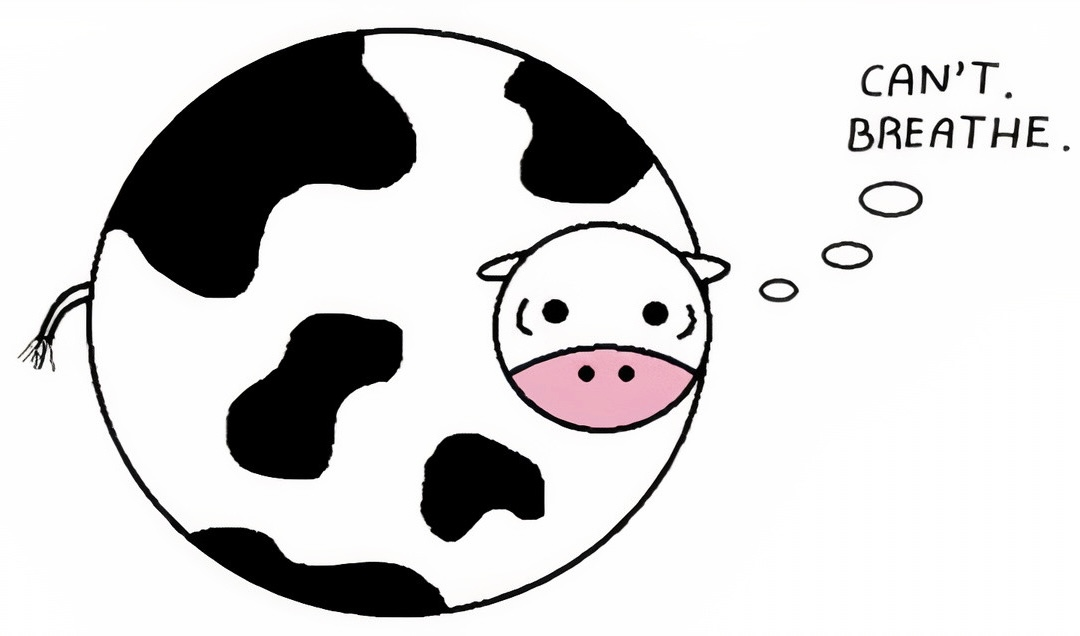
\includegraphics[width=0.9\textwidth]{Spherical cow}}} % Image background
\centering
\vspace*{0cm}
\par\normalfont\fontsize{35}{35}\sffamily\selectfont
\textbf{PHYS 2022 -- Modern Physics}\\
{\LARGE K. Yue}\par % Book title
\vspace*{1cm}
{\Huge Revision Notes}\par % Author name
\endgroup

% Copyright page

\newpage
~\vfill
\thispagestyle{empty}

\noindent \textsc{Hong Kong University of Science and Technology}\\
\noindent This set of revision notes is based on the series of PHYS 2022 lectures given by Prof. Yi Wang in 2021-22 Fall.\\ % License information

\noindent \textit{Second release, June 2023} % Printing/edition date

% Table of contents

\chapterimage{Contents} % Table of contents heading image

\pagestyle{empty} % No headers

\tableofcontents % Print the table of contents itself

% \cleardoublepage % Forces the first chapter to start on an odd page so it's on the right

\pagestyle{fancy} % Print headers again

\chapterimage{Introduction}
\addcontentsline{toc}{chapter}{Introduction}
\chapter*{Introduction}
This course aims to provide a brief overview of the advancement in Physics over the past century. Our journey begins at the theory of relativity, which encompasses two interrelated theories: special relativity and general relativity. The very basics of cosmology is then discussed. To get some idea of how the microscopic world works, we will have a glimpse at quantum mechanics. Subsequently, we will see the connection between the action principle and the laws of nature. Finally, the concept of entropy is introduced.\bigskip\newline
To allow readers quickly revise the materials covered in the course, some derivations are omitted. Problems and suggested solutions are provided at the end of each section for readers to consolidate their understanding. In the final section, a mock exam paper is given. Thanks to the lenient grading of the course, if you obtain around $85\%$ in the mock exam, I guarantee that you would at least get A range.\bigskip\newline
Last but not least, please do not distribute this set of notes to others unless you get the consent of the author, which is me. Otherwise, I would feel angry, sincerely hoping that you get a B+ or below in every course.

\section*{Acknowledgements}
I would like to thank everyone who has supported the production and refinement of this set of revision notes. I would like to express my special thanks to C. Ho, who notified me of the typos multiple times.

\chapterimage{Chapter 1} % Chapter heading image
\chapter{Special relativity}
Galileo's principle of relativity tells us that the laws of nature take the same form in all inertial frames. In other words,
\begin{itembox}
\begin{itemize}
\item Motion is relative.
\item Inertial frames are equivalent.
\item There is no absolute sense of ``who moves".
\item Laws of nature are invariant under a change from one inertial frame to another.
\end{itemize}
\end{itembox}
Applying the velocity addition rule in Newtonian mechanics, the speed of light can be different for different inertial frame. However, by solving the Maxwell's equations, we know that light propagates at a constant speed $c$ in the vacuum,
\begin{align*}
c\equiv\frac{1}{\sqrt{\mu_{0}\e_{0}}}
\end{align*}
where $\mu_{0}$ and $\e_{0}$ are the vacuum permeability and permittivity respectively. There must be something wrong.\bigskip\newline
To resolve such contradiction, Einstein developed special relativity by assuming the vacuum speed of light is $c$ in all inertial frames. This leads to two important results: time dilation and length contraction.

\section{Time dilation}
For an observer in an inertial frame of reference, a clock moving relative to him moves slower.
\begin{example}
Consider two observers, Alice and Bob. Alice is moving with velocity $v$ relative to Bob. In Alice's frame, the interval of the light clock is $\D t_{A}$. Alice's time interval measured by Bob is given by
\begin{eqnbox}
\begin{align}
\D t_{B}=\c\D t_{A}
\end{align}
\end{eqnbox}
where $\c$ is the Lorentz factor,
\begin{align*}
\c\equiv\frac{1}{\sqrt{1-\frac{v^2}{c^2}}}
\end{align*}
\end{example}

\section{Length contraction}
A moving object's length is measured to be shorter than its proper length.
\begin{example}
Consider the above problem again. This time, we put a ruler parallel to Alice's direction of motion on the ground. Wrt Bob, Alice has moved by distance $L=\c v\D t_{A}$. But from Alice's perspective, she moves with velocity $v$ for $\D t_{A}$, so she has moved by distance $L'=v\D t_{A}$. Therefore, the length of the ruler is contracted wrt Alice,
\begin{eqnbox}
\begin{align}
L'=\frac{L}{\c}
\end{align}
\end{eqnbox}
\end{example}

\section{Spacetime diagram}
On a spacetime diagram,
\begin{itembox}
\begin{itemize}
\item An event is a point.
\item Light travels at $45^\circ$ lines.
\item Except light, an object is a world line with slope greater than $45^\circ$ everywhere.
\item An inertial observer is a straight line.
\item A static object is a line parallel to the $ct$-axis.
\item Events at the same time are parallel to the $x$-axis.
\end{itemize}
\end{itembox}

\begin{minipage}[c]{0.4\textwidth}
    \centering
    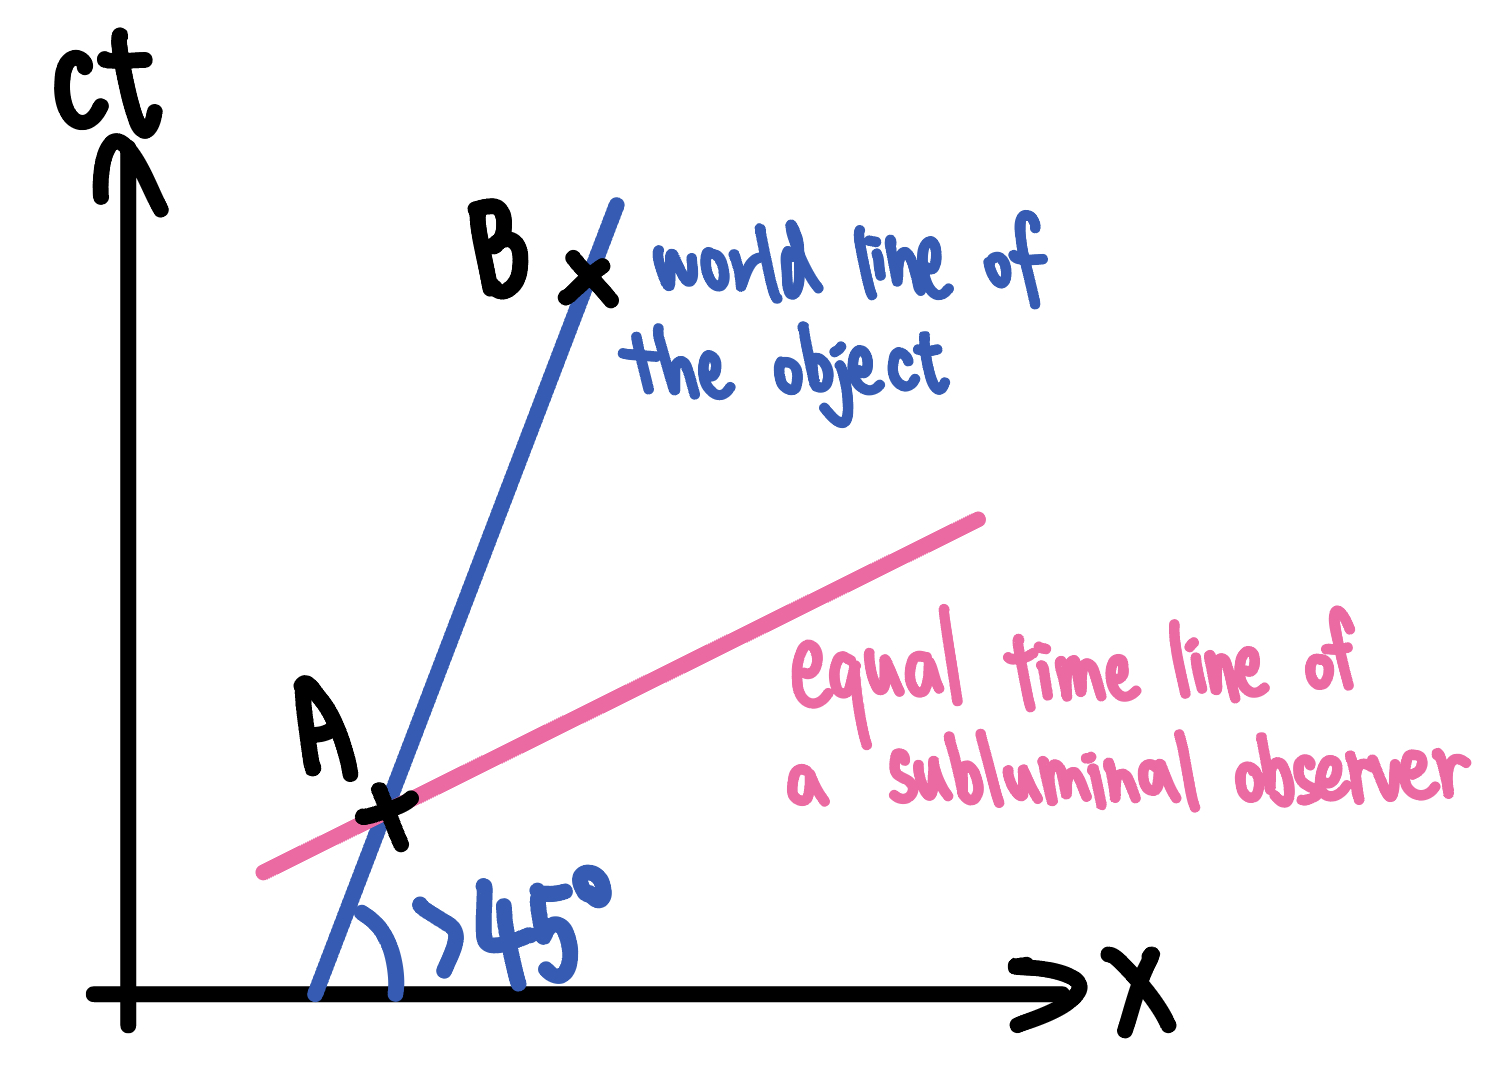
\includegraphics[width=\textwidth]{Spacetime diagram casuality}
\end{minipage}
\hfill
\begin{minipage}[c]{0.55\textwidth}
    \begin{example}
        Special relativity without superluminal motion is consistent with causality. On an object, an event $A$ leads to another event $B$. The world line of the object has slope greater than $45^\circ$, so a subluminal observer cannot flip the order of event $A$ and $B$. The cause-effect relation $A$ implying $B$ is preserved.
    \end{example}
\end{minipage}

\section{Lorentz transformation}
Alice is moving relative to Bob with velocity $v$ in the $+x$-direction. For simplicity, we choose the same origin of coordinate for Alice and Bob. Wrt Alice, the coordinate of a point is $\left(t_{A}, x_{A}\right)$, while that wrt Bob is $\left(t_{B}, x_{B}\right)$.\bigskip\newline
The transformation equations are
\begin{eqnbox}
\begin{align}
\begin{cases}
t_{A}=\c\left(t_{B}-\frac{v}{c^{2}}x_{B}\right)\\
x_{A}=\c\left(x_{B}-vt_{B}\right)\\
y_{A}=y_{B}\\
z_{A}=z_{B}
\end{cases}
&&
\begin{cases}
t_{B}=\c\left(t_{A}+\frac{v}{c^{2}}x_{A}\right)\\
x_{B}=\c\left(x_{A}+vt_{A}\right)\\
y_{B}=y_{A}\\
z_{B}=z_{A}
\end{cases}
\end{align}
\end{eqnbox}

\section{Spacetime interval}
In Euclidean space,
\begin{eqnbox}
\begin{align}
ds^{2}=-c^{2}dt^{2}+dx^{2}+dy^{2}+dz^{2}
\end{align}
\end{eqnbox}
The interval $ds^{2}$ is invariant under Lorentz transformation. The proof is trivial and left as an exercise to the reader (see \hyperref[The spacetime interval]{2020-21 Fall Midterm Q2 - The spacetime interval}).\bigskip\newline
The sign of $ds^{2}$ corresponds to three different types of separation of events,
\begin{eqnbox}
\begin{align}
\begin{split}
ds^{2}<0&\iff \text{time-like}\\
ds^{2}=0&\iff \text{light-like, null}\\
ds^{2}>0&\iff \text{space-like}\\
\end{split}
\end{align}
\end{eqnbox}
Space-like separated events cannot have cause-effect relation, since superluminal propagation is required to establish a cause-effect relation, which is forbidden in relativity.

\section{Relativistic momentum and energy}
Newtonian momentum and energy are not conserved in relativity. We have to search for new quantities that are consistent with Newtonian mechanics in the non-relativistic limit $v\ll c$.\bigskip\newline
We start with the definition of proper time,
\begin{align*}
d\t\equiv\sqrt{-\frac{ds^{2}}{c^2}}=\sqrt{dt^{2}-\frac{dx^{2}}{c^2}}=\frac{dt}{\c}
\end{align*}
The relativistic momentum is thus
\begin{eqnbox}
\begin{align}
\vec{p}\equiv m\frac{d\vec{x}}{d\t}=\c m\vec{v}
\end{align}
\end{eqnbox}
The definition of relativistic force immediately follows,
\begin{eqnbox}
\begin{align}
\vec{F}&\equiv\frac{d\vec{p}}{dt}\nonumber\\
&=\frac{d(\c m\vec{v})}{dt}\nonumber\\
&=m\c\dot{\vec{v}}+m\c^{3}\frac{\vec{v}(\vec{v}\cdot{\dot{\vec{v}}})}{c^2}
\end{align}
\end{eqnbox}
The relativistic energy is
\begin{eqnbox}
\begin{align}
E_{k}=\int_{0}^{x}F\,dx=(\c-1)mc^2
\end{align}
\end{eqnbox}
An object at rest has the relativistic rest energy
\begin{eqnbox}
\begin{align}
E_{r}=mc^2
\end{align}
\end{eqnbox}
Therefore, the total energy of an object is
\begin{eqnbox}
\begin{align}
E=E_{k}+E_{r}=\c mc^2
\end{align}
\end{eqnbox}

\addcontentsline{toc}{section}{Problems}
\section*{Problems}
\begin{problem}
Two events happen at the same time wrt Alice, and Bob is moving relative to Alice with velocity $v$. Given that the distance between two events is $L$ wrt Alice, calculate their time difference wrt Bob.
\end{problem}

\begin{solbox}
We can consider Bob to be moving in the $+x$-direction relative to Alice. The direction of Bob's motion does not matter since we only concern about the time difference between two events.\bigskip\newline
Wrt Alice, the coordinates of event 1 and event 2 are $\left(t_{1A}, x_{1A}\right)=(0,0)$ and $\left(t_{2A}, x_{2A}\right)=(0,L)$ respectively. Applying Lorentz transformation,
\begin{align*}
t_{1B}&=\c\left(t_{1A}-\frac{v}{c^{2}}x_{1A}\right)=0\\
t_{2B}&=\c\left(t_{2A}-\frac{v}{c^{2}}x_{2A}\right)=-\frac{\c vL}{c^{2}}
\end{align*}
The time difference between two events is $\D t=\frac{\c vL}{c^2}$.
\end{solbox}

\begin{problem}
Alice is moving relative to Bob with velocity $\vec{v}=(v, 0, 0)$. A ball moves with velocity $\vec{v}_{A}=(0,u,0)$ wrt Alice. Find its velocity $\vec{v}_{B}$ wrt Bob.
\end{problem}

\begin{solbox}
Applying Lorentz transformation,
\begin{align*}
t_{B}&=\c\left(t_{A}+\frac{v}{c^2}x_{A}\right)\\
x_{B}&=\c\left(x_{A}+vt_{A}\right)
\end{align*}
Note that $\vec{v}_{B}=\left(\frac{dx_{B}}{dt_{B}},\frac{dy_{B}}{dt_{B}},\frac{dz_{B}}{dt_{B}}\right)$,
\begin{align*}
\frac{dx_{B}}{dt_{B}}&=\frac{\c d\left(x_{A}+vt_{A}\right)}{\c d\left(t_{A}+\frac{v}{c^2}x_{A}\right)}\\
&=\frac{dx_{A}+vdt_{A}}{dt_{A}+\frac{v}{c^2}dx_{A}}\\
&=\frac{v_{Ax}+v}{1+\frac{v_{Ax}v}{c^2}}\\
&=v
\end{align*}
Similarly, 
\begin{align*}
\frac{dy_{B}}{dt_{B}}&=\frac{v_{Ay}}{\c\left(1+\frac{v_{Ax}v}{c^2}\right)}=\frac{u}{\c}\\
\frac{dz_{B}}{dt_{B}}&=\frac{v_{Az}}{\c\left(1+\frac{v_{Ax}v}{c^2}\right)}=0
\end{align*}
Combining the results, $\vec{v}_{B}=\left(v, \frac{u}{\c}, 0\right)$.
\end{solbox}

\begin{problem}
Verify eq. (1.8).
\end{problem}
\begin{solbox}
\begin{align*}
E_{k}&=\int_{0}^{x}F\,dx\\
&=\int_{0}^{x}\frac{d\left(\c mv\right)}{dt}\,dx\\
&=\int_{0}^{v} v\,d\left(\c mv\right)\\
&=\c mv^{2}\big|^{v}_{0}-\int_{0}^{v} \c mv\,dv\\
&=\c mv^{2}-m\int_{0}^{v} \frac{v}{\sqrt{1-\frac{v^2}{c^2}}}\,dv\\
&=\c mv^{2}+mc^{2}\left(\sqrt{1-\frac{v^2}{c^2}}-1\right)\\
&=\frac{mv^2}{\sqrt{1-\frac{v^2}{c^2}}}+mc^{2}\cdot\frac{1-\frac{v^2}{c^2}-\sqrt{1-\frac{v^2}{c^2}}}{\sqrt{1-\frac{v^2}{c^2}}}\\
&=\left(\c-1\right)mc^2
\end{align*}
\end{solbox}

\subsection*{2019-20 Fall Midterm Q2 - Relativistic kinetic energy and momentum}
In Newtonian mechanics, the relation between kinetic energy and momentum is $E_{k}=\frac{p^2}{2m}$.\bigskip\newline
a) Find its relativistic generalization (a relation between $E$, $p$, $m$ and $c$).\bigskip\newline
b) Verify that the kinetic energy is consistent with the Newtonian relation above in the non-relativistic limit.

\begin{solbox}
a) The relativistic energy of a point mass $m$ moving at speed $v$ is
\begin{align}
E=\c mc^{2}\nonumber
\end{align}
and the relativistic momentum is
\begin{align}
p=\c mv\nonumber
\end{align}
Combining these two equations,
\begin{align}
E^2=m^2 c^4+p^2 c^2\nonumber
\end{align}
I suggest you memorize this result.\bigskip\newline
b)
\begin{align*}
E_{k}&=E-mc^2\\
&=\sqrt{m^2 c^4+p^2 c^2}-mc^2
\end{align*}
In the non-relativistic limit, $p\ll mc$, 
\begin{align*}
\sqrt{m^2 c^4+p^2 c^2}-mc^2&=mc^2{\left(1+\frac{p^2}{m^2 c^2}\right)}^{\frac{1}{2}}-mc^2\\
&\approx mc^2\left(1+\frac{1}{2}\frac{p^2}{m^2 c^2}\right)-mc^2\\
&=\frac{p^2}{2m}
\end{align*}
We get back the Newtonian relation $E_{k}=\frac{p^2}{2m}$.
\end{solbox}

\subsection*{2019-20 Fall Midterm Q3 - The ladder paradox}
\label{The ladder paradox}
Alice moves with a ladder with speed $v=0.87c$ towards a garage at rest, and Bob is standing with the garage. The static length of the ladder and the garage are $15\text{m}$ and $10\text{m}$ respectively. 
\begin{figure}[H]
\centering
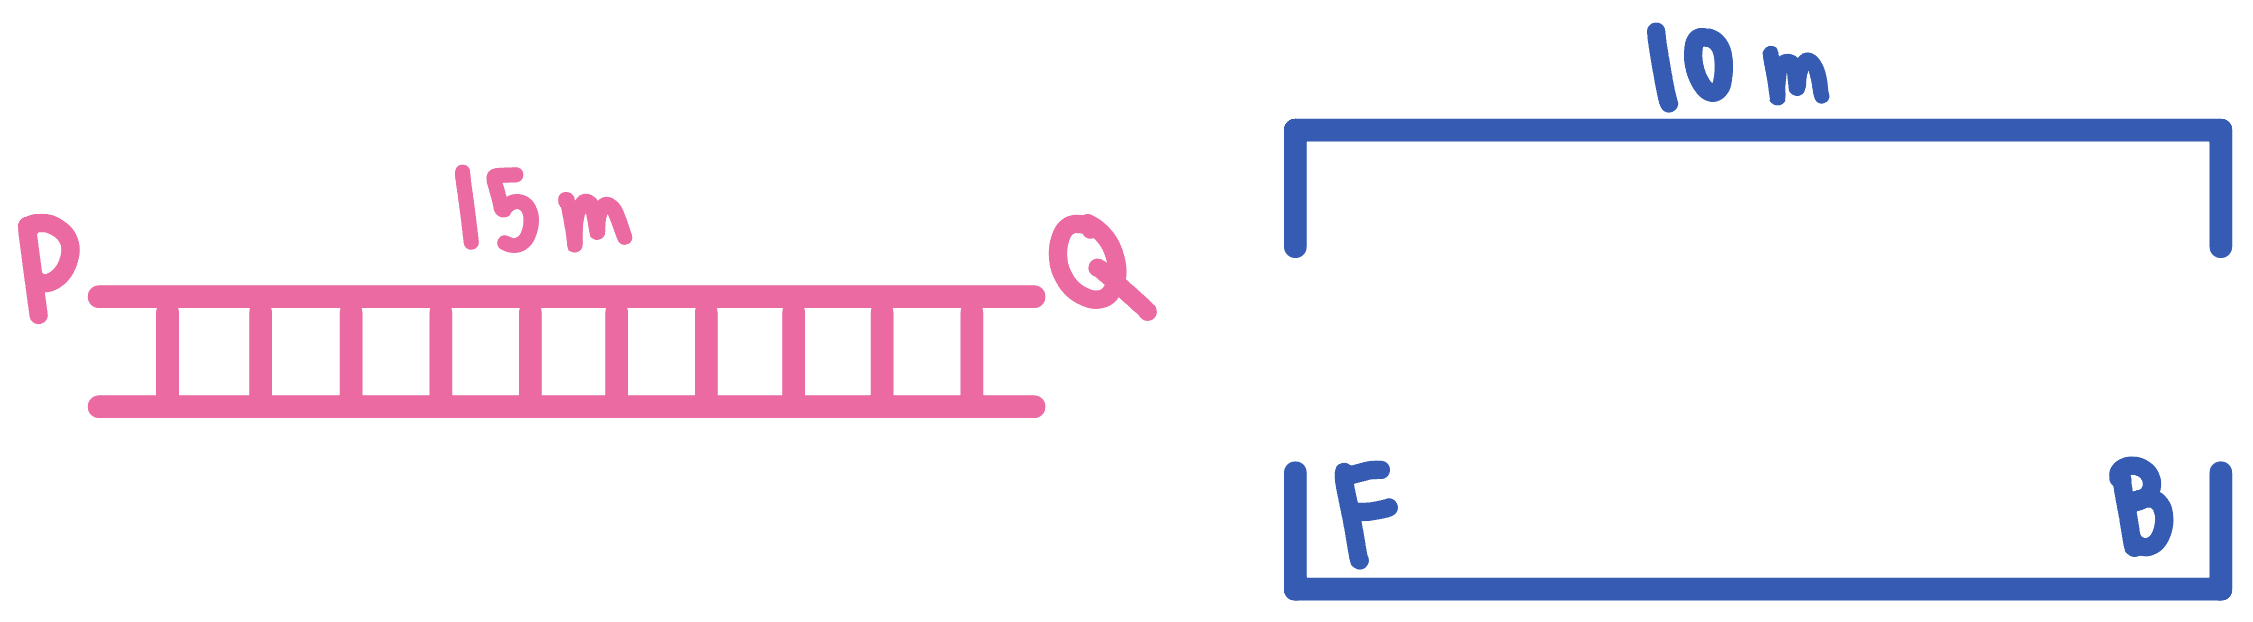
\includegraphics[width=0.65\textwidth]{Ladder paradox}
\end{figure}
\noindent a) Draw the spacetime diagram of Bob's frame, and use it to explain whether the ladder fits into the garage wrt both Alice and Bob respectively.\bigskip\newline
b) Draw the spacetime diagram of Alice's frame, and use it to explain whether the ladder fits into the garage wrt both Alice and Bob respectively.

\begin{solbox}
The Lorentz factor is
\begin{align*}
\c&=\frac{1}{\sqrt{1-\frac{v^2}{c^2}}}\\
&=2
\end{align*}
The angle $\theta$ between the $ct_{A}$-axis and $ct_{B}$-axis is
\begin{align*}
\theta&=90^\circ-\tan^{-1}\left(\frac{c}{v}\right)\\
&=41.0^\circ
\end{align*}
a) In Bob's frame, the ladder shrinks to $\frac{L_{l}}{\c}=7.5\text{m}<L_{g}$, so he thinks the ladder can fit into the garage. In Alice's frame, the ladder shrinks to $\frac{L_{g}}{\c}=5\text{m}<L_{l}$, so she thinks the garage cannot hold the ladder. They are both correct since ``ladder fits in garage" is not an event localized at a spacetime point. It can be separated into two events.\bigskip\newline
$1$: P enters front door F.\\
$2$: Q exits back door B.\bigskip\newline
The two events are space-like separated and has no causality, thus their order can be swapped. For Bob, event 1 happens before event 2, while for Alice, event 2 happens before event 1.\bigskip\newline
\begin{figure}[H]
\centering
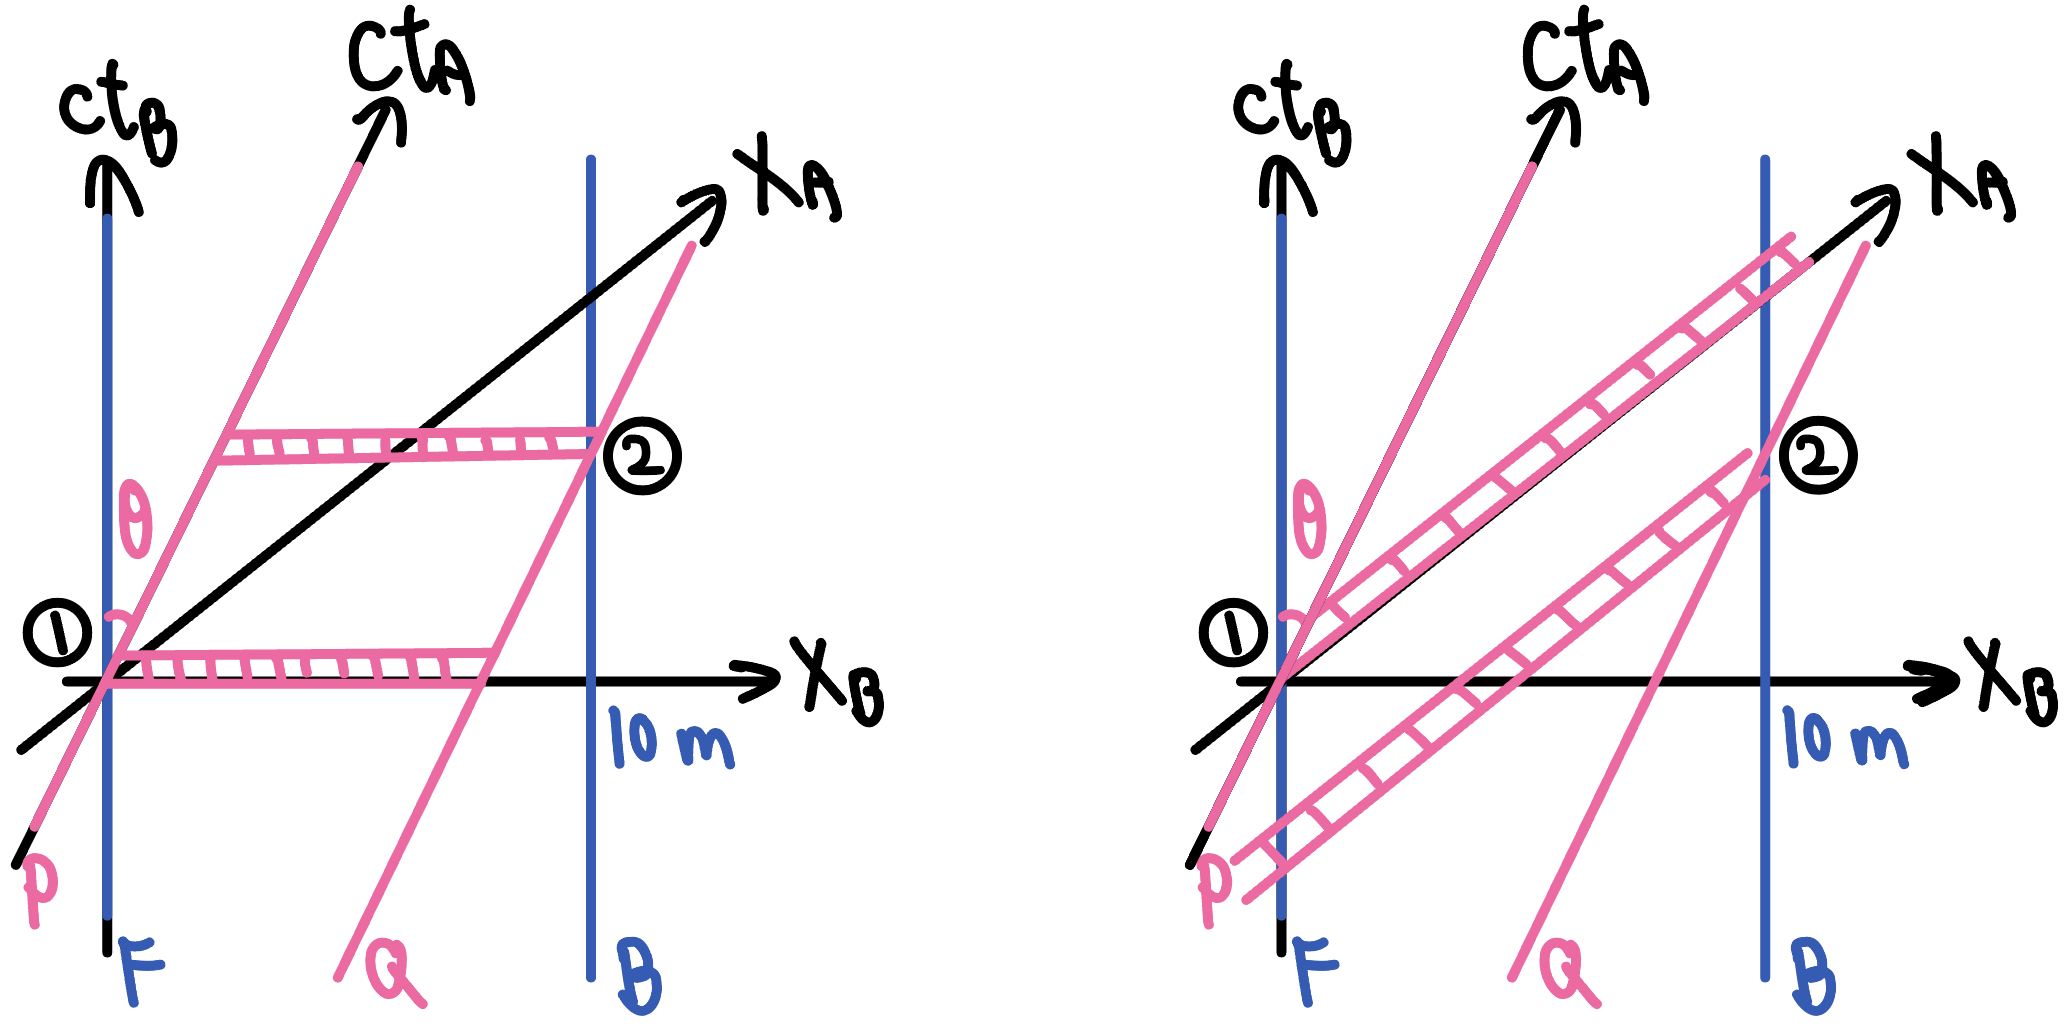
\includegraphics[width=0.7\textwidth]{Bob's spacetime diagram}
\caption{Spacetime diagram in Bob's frame, left: Bob's interpretation; right: Alice's interpretation.}
\end{figure}
\bigskip
\noindent b) The explanation is same as (a).
\begin{figure}[H]
\centering
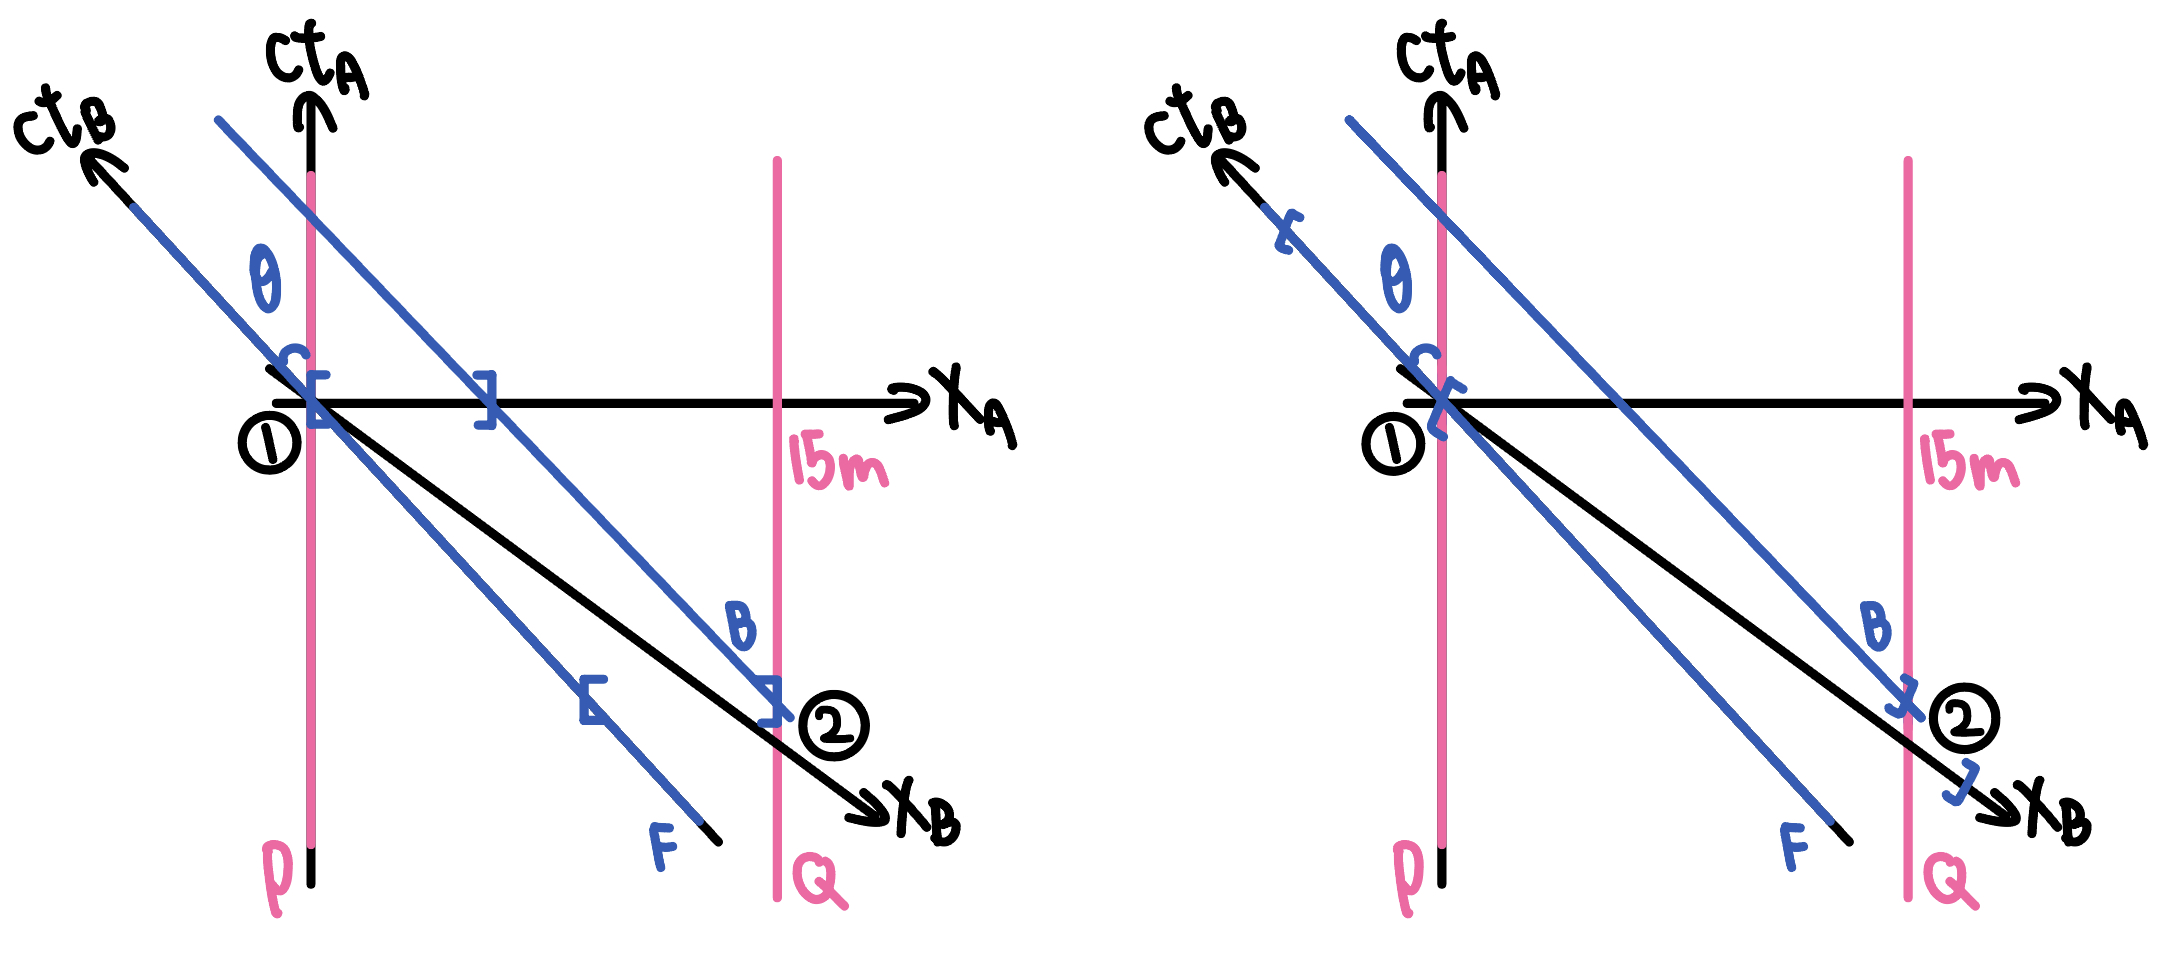
\includegraphics[width=0.775\textwidth]{Alice's spacetime diagram}
\caption{Spacetime diagram in Alice's frame, left: Alice's interpretation; right: Bob's interpretation.}
\end{figure}
\end{solbox}

\subsection*{2019-20 Fall Midterm Q4 - Relativistic velocity addition}
Alice is moving away from Bob with velocity $\vec{v}=\left(0, 0, v\right)$, and sends out a light ray.\bigskip\newline
a) If the light ray is along the $x$-direction wrt Alice, calculate its velocity $\vec{v}_{B}$ wrt Bob.\bigskip\newline
b) If the light ray is along the $z$-direction wrt Alice, calculate its velocity $\vec{v}_{B}$ wrt Bob.\bigskip\newline
c) Assuming Alice sends out light rays in (a) and (b) with the same frequency, which light has higher frequency wrt Bob?\bigskip\newline
d) Show explicitly that for the light ray in any direction, as long as the speed of light is $c$ in Alice's frame, the speed of light is still $c$ wrt Bob.

\begin{solbox}
a) In Alice's frame, $\vec{v}_{A}=\left(c, 0, 0\right)$. With reference to Problem 1.2,
\begin{align*}
v_{Bx}&=\frac{v_{Ax}}{\c\left(1+\frac{v_{Az}v}{c^2}\right)}=\sqrt{1-\frac{v^2}{c^2}}\cdot c=\sqrt{c^2-v^2}\\
v_{By}&=\frac{v_{Ay}}{\c\left(1+\frac{v_{Az}v}{c^2}\right)}=0\\
v_{Bz}&=\frac{v_{Az}+v}{1+\frac{v_{Az}v}{c^2}}=v
\end{align*}
b) In Alice's frame, $\vec{v}_{A}=\left(0, 0, c\right)$.
\begin{align*}
v_{Bx}&=\frac{v_{Ax}}{\c\left(1+\frac{v_{Az}v}{c^2}\right)}=0\\
v_{By}&=\frac{v_{Ay}}{\c\left(1+\frac{v_{Az}v}{c^2}\right)}=0\\
v_{Bz}&=\frac{v_{Az}+v}{1+\frac{v_{Az}v}{c^2}}=\frac{c+v}{1+\frac{cv}{c^2}}=c
\end{align*}
c) The frequency in (b) is higher due to Doppler effect.\bigskip\newline
d) For convenience, we use spherical coordinates to define an arbitrary direction of $\vec{v}_{A}$.\bigskip\newline
In Alice's frame, we let $\vec{v}_{A}=\left(c\sin\theta\cos\phi, c\sin\theta\sin\phi, c\cos\theta\right)$, where $\theta$ is the polar angle and $\phi$ is the azimuthal angle (the usual convention in Mathematics is different: $\phi$ is the polar angle and $\theta$ is the azimuthal angle).
\begin{align*}
v_{Bx}&=\frac{v_{Ax}}{\c\left(1+\frac{v_{Az}v}{c^2}\right)}=\frac{\sqrt{1-\frac{v^2}{c^2}}c\sin\theta\cos\phi}{1+\frac{v\cos\theta}{c}}\\
v_{By}&=\frac{v_{Ay}}{\c\left(1+\frac{v_{Az}v}{c^2}\right)}=\frac{\sqrt{1-\frac{v^2}{c^2}}c\sin\theta\sin\phi}{1+\frac{v\cos\theta}{c}}\\
v_{Bz}&=\frac{v_{Az}+v}{1+\frac{v_{Az}v}{c^2}}=\frac{c\cos\theta+v}{1+\frac{v\cos\theta}{c}}
\end{align*}
Therefore, the speed of light in Bob's frame is still $c$,
\begin{align*}
\left|\vec{v}_{B}\right|^{2}&=v_{Bx}^{2}+v_{By}^{2}+v_{Bz}^{2}\\
&=\frac{\left(1-\frac{v^{2}}{c^{2}}\right)c^{2}\sin^{2}\theta\cos^{2}\phi}{\left(1+\frac{v\cos\theta}{c}\right)^{2}}+\frac{\left(1-\frac{v^{2}}{c^{2}}\right)c^{2}\sin^{2}\theta\sin^{2}\phi}{\left(1+\frac{v\cos\theta}{c}\right)^{2}}+\frac{\left(c\cos\theta+v\right)^{2}}{\left(1+\frac{v\cos\theta}{c}\right)^{2}}\\
&=\frac{\left(1-\frac{v^{2}}{c^{2}}\right)c^{2}\sin^{2}\theta}{\left(1+\frac{v\cos\theta}{c}\right)^{2}}+\frac{\left(c\cos\theta+v\right)^{2}}{\left(1+\frac{v\cos\theta}{c}\right)^{2}}\\
&=c^{2}
\end{align*}
\end{solbox}

\subsection*{2020-21 Fall Midterm Q2 - The spacetime interval}
\label{The spacetime interval}
In Alice's frame, for the interval between two nearby events, we have $ds^2=-c^2 dt_{A}^2+dx_{A}^2$. Bob is moving relative to Alice with velocity $v$ in the $+x$-direction.\bigskip\newline
a) Find $t_{B}$ and $x_{B}$ in Bob's frame.\bigskip\newline
b) Find $ds^2$ in terms of $c$, $dt_{B}$ and $dx_{B}$.

\begin{solbox}
a) Applying Lorentz transformation,
\begin{align*}
t_{B}&=\c\left(t_{A}-\frac{v}{c^2}x_{A}\right)=\frac{\left(t_{A}-\frac{v}{c^2}x_{A}\right)}{\sqrt{1-\frac{v^2}{c^2}}}\\
x_{B}&=\c\left(x_{A}-vt_{A}\right)=\frac{x_{A}-vt_{A}}{\sqrt{1-\frac{v^2}{c^2}}}
\end{align*}
b) We guess $ds^2=-c^2dt_{B}^2+dx_{B}^2$.
\begin{align*}
-c^2dt_{B}^2+dx_{B}^2&=-c^2{\c}^2d\left(t_{A}^2-\frac{2v}{c^2}t_{A}x_{A}+\frac{v^2}{c^4}x_{A}^2\right)+{\c}^2 d\left(x_{A}^2-2vt_{A}x_{A}+v^2 t_{A}^2\right)\\
&=-c^2 {\c}^2dt_{A}^2+2{\c}^2 vd\left(t_{A}x_{A}\right)-\frac{{\c}^2 v^2}{c^2}dx_{A}^2+{\c}^2 dx_{A}^2-2{\c}^2 vd\left(t_{A}x_{A}\right)+{\c}^2 v^2dt_{A}^2\\
&=-c^2 dt_{A}^2+dx_{A}^2\\
&=ds^2
\end{align*}
We can generalize the result to any arbitrary direction of $\vec{v}$ in three-dimensional space by rotational invariance. This proves the interval $ds^2$ is Lorentz invariant.
\end{solbox}

\subsection*{2020-21 Fall Midterm Q3 - Collision of particles}
A massive particle A with rest mass $m$ collides head-on with a massless particle B in $1$ space dimension. Before the collision, B has energy $Q$. After the collision, B still has energy $Q$, but it is moving in the opposite direction. Express the quantities below using $m$, $c$ and $Q$.\bigskip\newline
a) What is the relativistic momentum of B before and after the collision?\bigskip\newline
b) What is the relativistic momentum and energy of A before and after the collision?\bigskip\newline
c) What is the speed of A before and after the collision?

\begin{solbox}
a) Suppose A is initially moving towards the right and B towards the left. 
\begin{align*}
E_{B}&=\left|p_{B}\right|c=Q\\
p_{B}&=\mp \frac{Q}{c}
\end{align*}
where ``$-$'' sign is before collision and ``$+$'' sign is after collision (the overall $\mp$ sign depends on the choice of coordinates, the answer is correct as long as there is a relative sign difference).\bigskip\newline
b) By momentum conservation,
\begin{align*}
p_{A}+p_{B}&=0\\
p_{A}&=-p_{B}=\pm\frac{Q}{c}
\end{align*}
where ``$+$" sign is before collision and ``$-$'' sign is after collision.\bigskip\newline
The energy of A can be obtained from the dispersion relation,
\begin{align*}
E_{A}&=\sqrt{p_{A}^{2}c^{2}+m^2 c^4}\\
&=\sqrt{Q^2+m^2 c^4}
\end{align*}
It is the same before and after collision.\bigskip\newline
c) The expression of relativistic energy is $E_{A}=\c mc^2$. Using the result in (b),
\begin{align*}
\sqrt{Q^2+m^2 c^4}&=\c mc^2\\
\frac{1}{\sqrt{1-\frac{v^2}{c^2}}}&=\frac{\sqrt{Q^2+m^2 c^4}}{mc^2}
\end{align*}
After solving,
\begin{align*}
v=\pm\frac{cQ}{\sqrt{Q^2+m^2 c^4}}
\end{align*}
where ``$+$" sign is before collision and ``$-$" sign is after collision.
\end{solbox}

\subsection*{2022-23 Fall Midterm Q2 - Energy and speed of an electron}
The electron mass is $m_{e}=0.5\text{MeV/}\text{c}^{2}$. Now a moving electron has total energy 1MeV. What is its speed?
\begin{solbox}
The total energy is
\begin{align*}
    E=\c m_{e}c^2\implies \c=\frac{E}{m_{e}c^2}=2
\end{align*}
The speed $v$ is given by
\begin{align*}
\c=\frac{1}{\sqrt{1-\frac{v^2}{c^2}}}\implies v=\sqrt{\frac{3}{2}}c
\end{align*}
Using the momentum $p$ to solve for $v$ is also acceptable.
\end{solbox}

\subsection*{2022-23 Fall Midterm Q3 - Time difference in different frames}
Consider points M, P, Q at rest in B' s frame. The distances $|PM|=|MQ|=L$. Now from M, two beams of light are emitted at the same time to the left and right. Consider the light arrival time to points P and Q.
\begin{figure}[H]
    \centering
    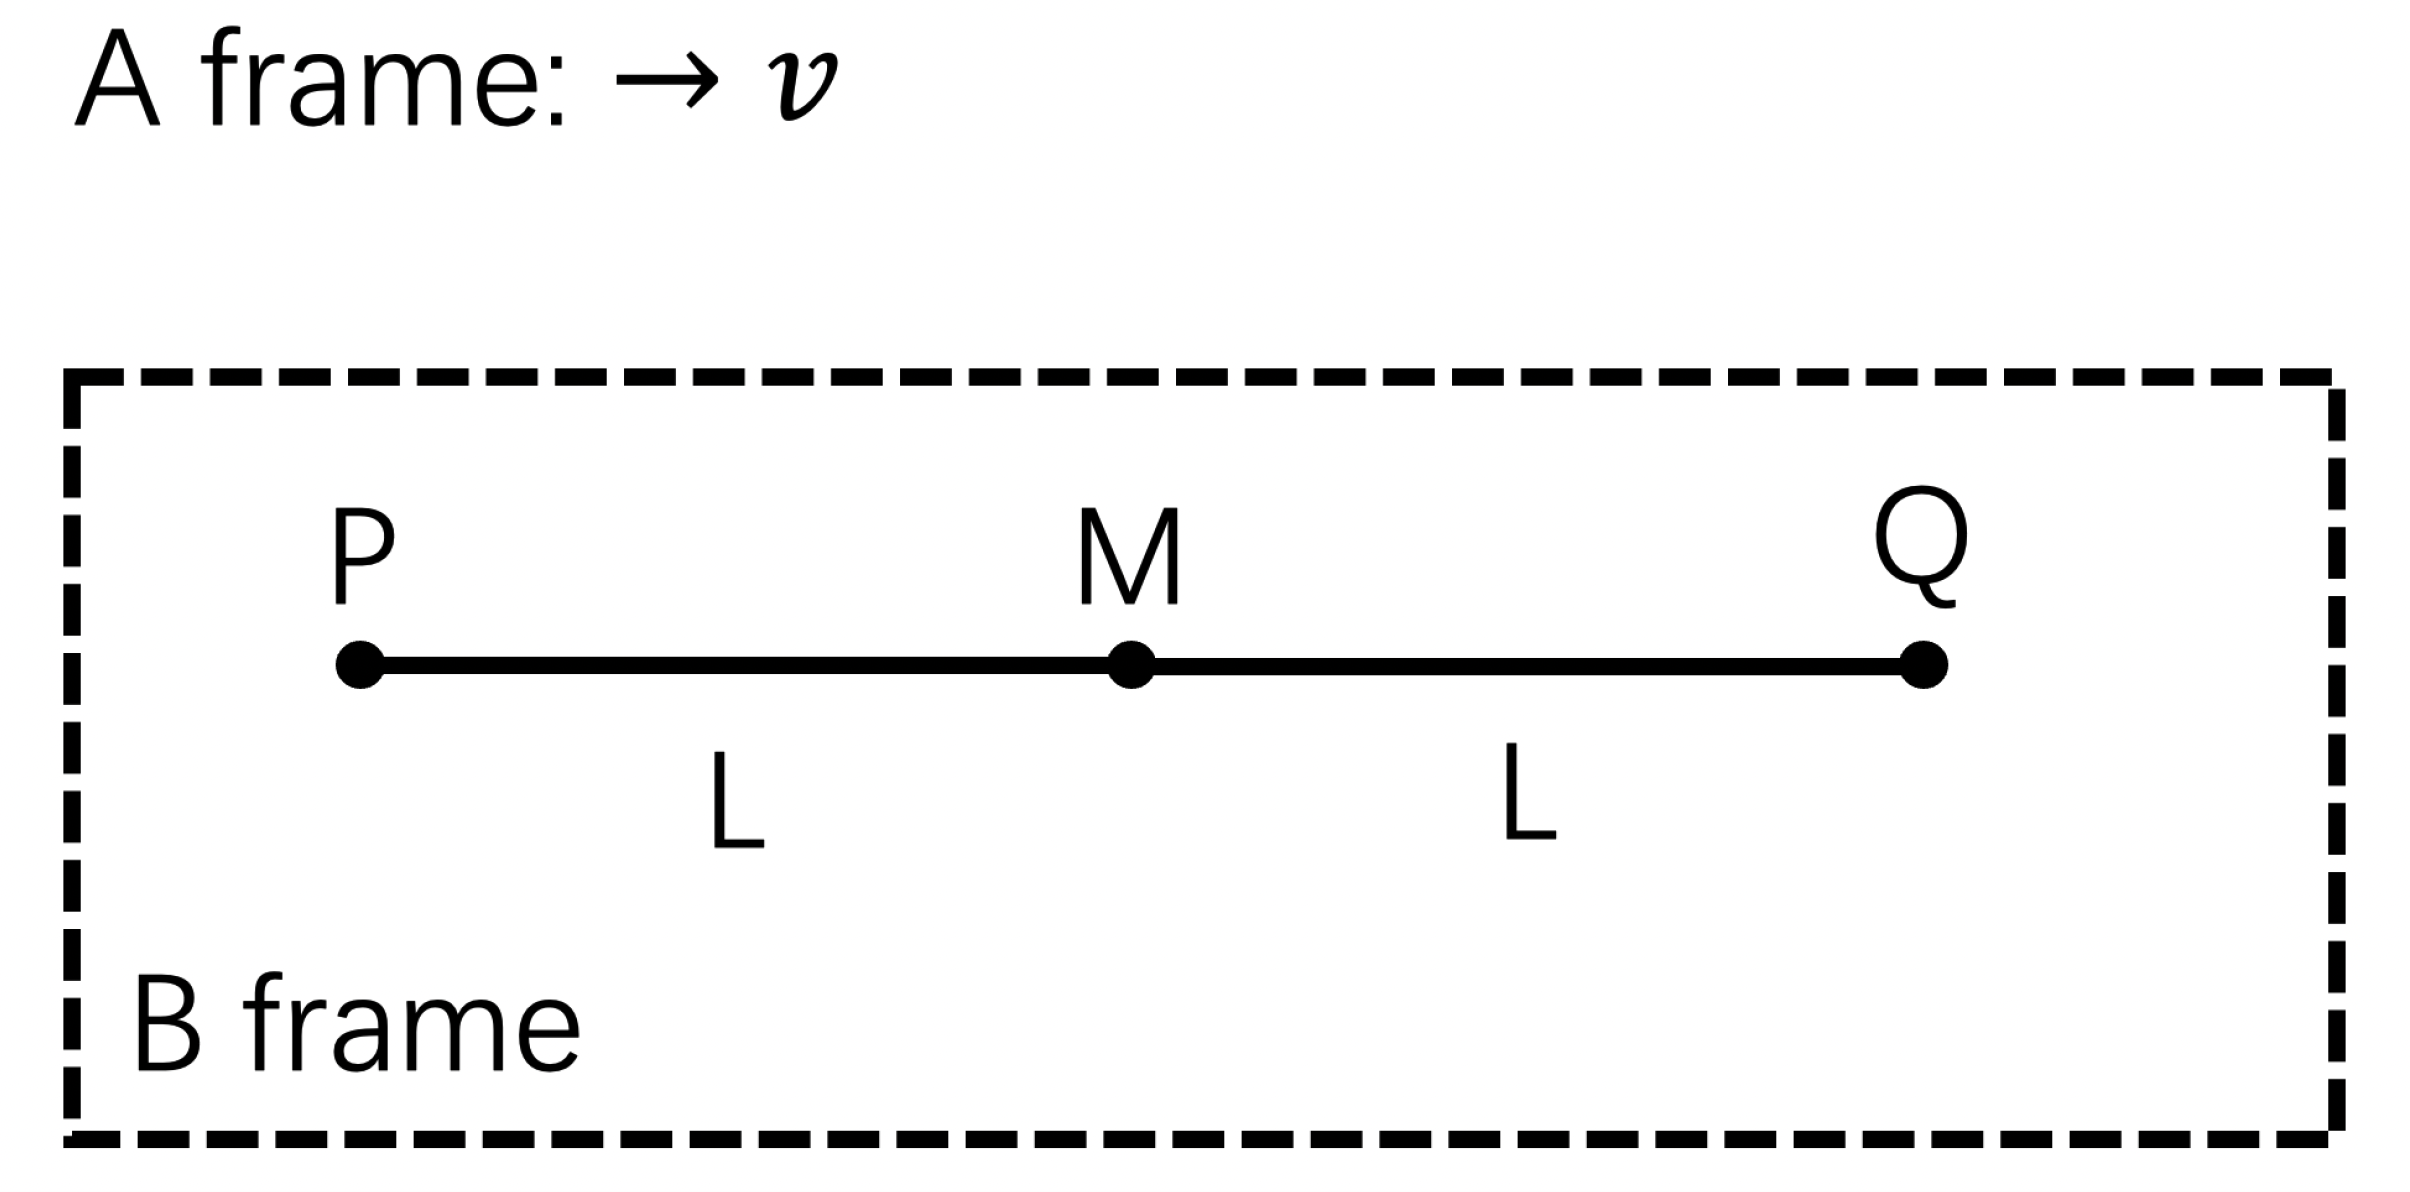
\includegraphics[width=0.5\textwidth]{Time difference in different frames}
\end{figure}
\noindent a) What is the arrival time difference of the two signals in B's frame?\bigskip\newline
b) Consider A running to the right with speed $v$. In A's frame, which is earlier? Light arrival to P or light arrival to Q?\bigskip\newline
c) What is the arrival time difference of the two signals in A's frame?
\begin{solbox}
a) In B's frame, the arrival time difference of two signals is
\begin{align*}
\Delta t&= t_{P}-t_{Q}\\
&=\frac{L}{c}-\frac{L}{c}\\
&=0
\end{align*}
Since the setup is left-right symmetric, there is no time difference between the arrival of the signals at P and Q.\bigskip\newline
b) The light arrival at Q will be earlier.\bigskip\newline
c) In B's frame, two arriving events of P and Q happen at the same time: $t_{B, P}=t_{B, Q}=\frac{L}{c}$. Consider A to be moving relative to B with velocity $v$ in the $+x$-direction. Applying Lorentz transformation,
\begin{align*}
t_{A, P}&=\c\left(t_{B, P}-\frac{v}{c^2}x_{A, P}\right)=\frac{\c vL}{c}\left(1+\frac{v}{c}\right)\\
t_{A, Q}&=\c\left(t_{B, Q}-\frac{v}{c^2}x_{A, Q}\right)=\frac{\c vL}{c}\left(1-\frac{v}{c}\right)
\end{align*}
In A's frame, the light arrival at Q will be earlier since $t_{A,Q}<t_{A,P}$. The time difference is
\begin{align*}
\Delta t=t_{A,P}-t_{A,Q}=\frac{2\c vL}{c^2}
\end{align*}
\end{solbox}

\newpage
\chapterimage{Chapter 2} % Chapter heading image
\chapter{General relativity}
The inertial mass $m_{I}$ and gravitational mass $m_{G}$ are from different origin.
\begin{itembox}
\begin{itemize}
\item Inertial mass $m_{I}=\frac{F}{a}$ is a measure of inertia.
\item Gravitational mass $m_{G}=\frac{F}{g}$ is related to how strongly gravity attracts the matter.
\end{itemize}
\end{itembox}
Experiments suggest that $m_{I}=m_{G}$, and the equivalence between these two quantities is explained by Einstein's general relativity.

\section{Einstein's equivalence principle}
Einstein asserted that for uniform gravitational field,\bigskip\newline
``We ... assume the complete physical equivalence of a (uniform) gravitational field and a corresponding acceleration of the reference frame".\bigskip\newline
This assumption explains why $m_{I}=m_{G}$, because inertia (acceleration) equals gravity.\bigskip\newline
Uniform gravity $g$ can thus be cancelled by constant acceleration $a=g$. If gravity is not uniform, we can apply the equivalence principle to cancel gravity locally at a point.

\section{Light bending effect}
With the equivalence principle, we immediately know that light bends the same way as in an accelerated environment.
\begin{example}
A person standing in front of you appears slightly taller because the Earth's gravity has the effect of light bending.
\end{example}
\noindent However, the light bending effect cannot be accounted for by the equivalence principle alone. The geometric effect contributes another equal amount.

\section{Time with uniform gravity}
Alice stands higher by a vertical distance $h$ than Bob, and the gravitational acceleration is $g$. Alice experiences a faster time than Bob,
\begin{eqnbox}
\begin{align}
\D t_{A}=\left(1+\frac{gh}{c^2}\right)\D t_{B}
\end{align}
\end{eqnbox}
In the weak field limit, eq. (2.1) can be generalized for Alice and Bob in two different gravitational potential $\phi_{A}$ and $\phi_{B}$,
\begin{eqnbox}
\begin{align}
dt_{A}=\left(1+\frac{\phi_{A}-\phi_{B}}{c^2}\right)dt_{B}
\end{align}
\end{eqnbox}

\section{Schwarzschild metric}
Consider a spherical star with mass $M$, the Schwarzschild metric describes the spacetime geometry outside the star,
\begin{eqnbox}
\begin{align}
ds^2=-\left(1-\frac{r_{s}}{r}\right)c^2 dt^2+{\left(1-\frac{r_{s}}{r}\right)}^{-1} dr^2+r^2 \left(d\theta^{2}+\sin^{2}\theta d\phi^{2}\right)
\end{align}
\end{eqnbox}
where $r_{s}=\frac{2GM}{c^2}$ is the Schwarzschild radius.

\section{Black holes}
When an object is so dense that its size is smaller than its Schwarzschild radius $r_{s}$, it forms a black hole. Imagine that Alice is staying at a fixed distance $r$ very slightly greater than $r_{s}$, while Bob is at $r\to\infty$. For any finite interval $\D t_{A}$ experienced by Alice, 
\begin{eqnbox}
\begin{align}
\D t_{B}={\left(1-\frac{r_{s}}{r}\right)}^{-\frac{1}{2}}\D t_{A}\to\infty
\end{align}
\end{eqnbox}
Bob finds Alice frozen on the $r=r_{\text{s}}$ surface. Due to extreme time dilation, the light emitted at $r_{s}$ takes infinite time to reach Bob, so Bob cannot see events at $r<r_{\text{s}}$. Thus, $r=r_{\text{s}}$ is a surface that limits the events Bob can see, and it is known as the event horizon.\bigskip\newline
At $r<r_{s}$, the Schwarzschild metric becomes
\begin{align}
ds^2=-{\left(\frac{r_{s}}{r}-1\right)}^{-1}dr^2 +\left(\frac{r_{s}}{r}-1\right)c^2 dt^2+r^2 \left(d\theta^{2}+\sin^{2}\theta d\phi^{2}\right)\nonumber
\end{align}
$dr$ becomes time-like and $dt$ becomes space-like. Therefore, for everything inside the black hole, the $-r$ direction now becomes the time direction, and it has no choice other than moving along the time direction towards the singularity $r=0$. The singularity is the future of the observer at finite time.

\section{Gravitational waves}
Gravitational waves are the fluctuations of spacetime. They propagate at the speed of light and they are transverse waves, i.e. polarized orthogonal to the propagation direction.\bigskip\newline
Gravitational waves distort distances and hence can be observed, albeit with great difficulty. After decades of failure, gravitational waves are finally detected by the Laser Interferometer Gravitational-Wave Observatory (LIGO) in 2016. 
\begin{figure}[H]
\centering
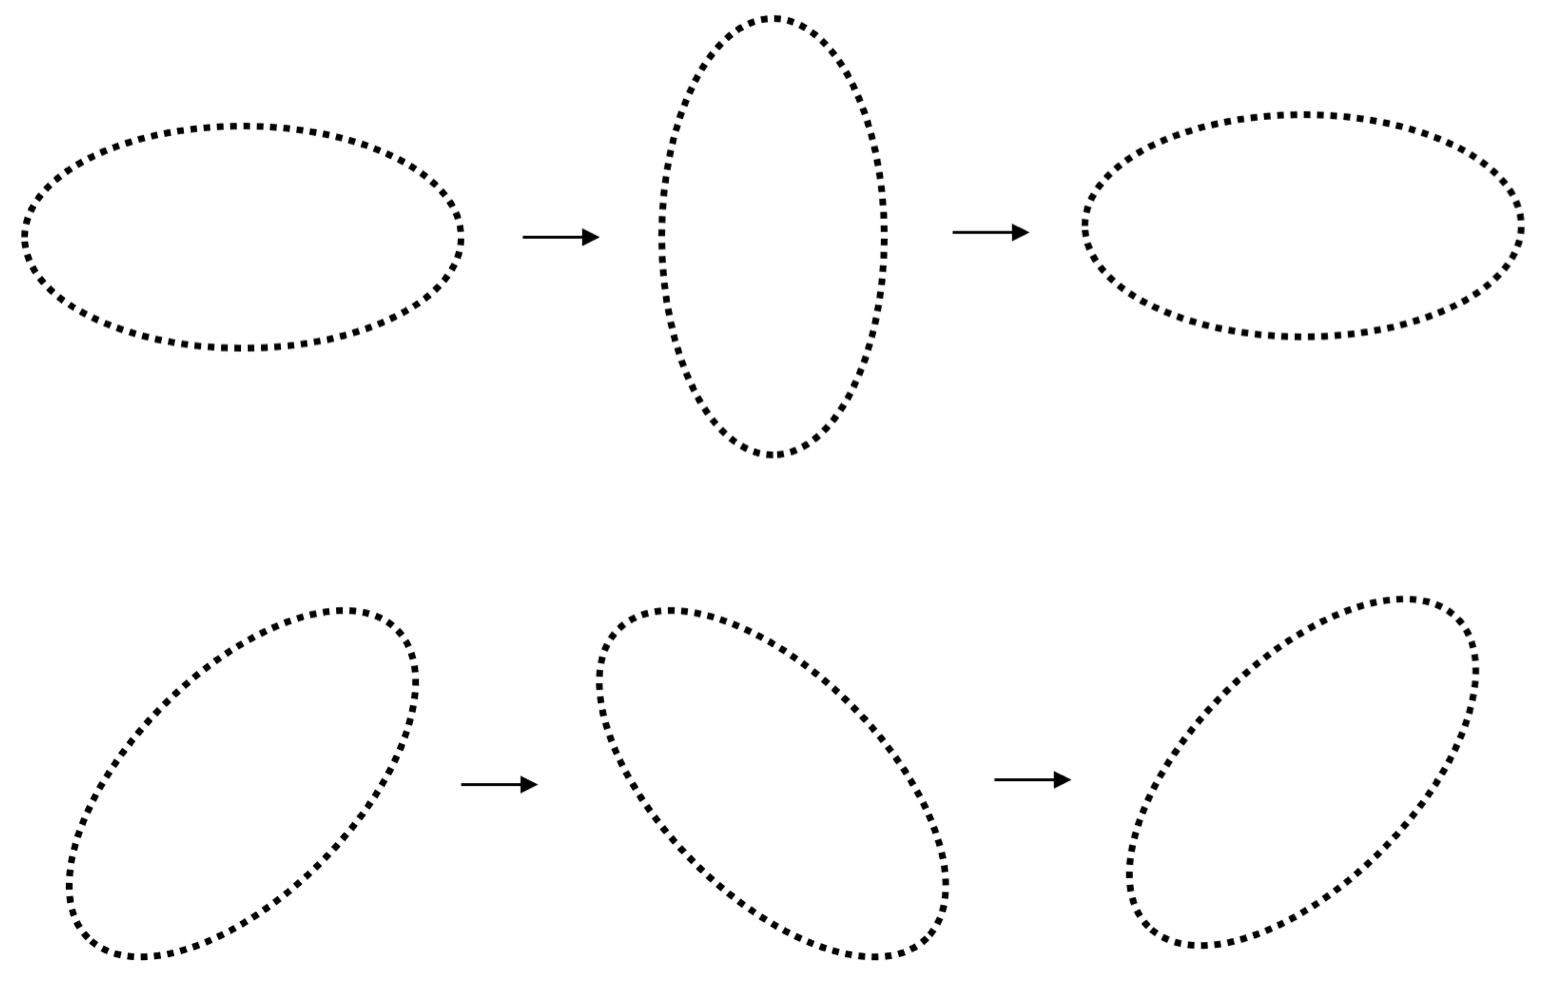
\includegraphics[width=0.5\textwidth]{Gravitational waves}
\caption{Two polarization modes of gravitational waves}
\end{figure}

\addcontentsline{toc}{section}{Problems}
\section*{Problems}
\begin{problem}
Show that eq. (2.4) is consistent with eq. (2.2) when $r_{A}, r_{B}\gg r_{s}$.
\end{problem}
\begin{solbox}
We take $\phi=0$ at $r\to\infty$. Using eq. (2.4),
\begin{align*}
\D t&={\left(1-\frac{r_{s}}{r_{A}}\right)}^{-\frac{1}{2}}\D t_{A}\\
\D t&={\left(1-\frac{r_{s}}{r_{B}}\right)}^{-\frac{1}{2}}\D t_{B}
\end{align*}
where $\D t$ is the standard time interval at $r\to\infty$. Combining these two equations,
\begin{align*}
dt_{A}&={\left(1-\frac{r_{s}}{r_{A}}\right)}^{\frac{1}{2}}{\left(1-\frac{r_{s}}{r_{B}}\right)}^{-\frac{1}{2}}dt_{B}\\
&\approx \left(1-\frac{r_{s}}{2r_{A}}\right)\left(1+\frac{r_{s}}{2r_{B}}\right)dt_{B}\\
&\approx \left(1-\frac{r_{s}}{2r_{A}}+\frac{r_{s}}{2r_{B}}\right)\\
&=\left(1-\frac{GM}{r_{A}c^2}+\frac{GM}{r_{B}c^2}\right)
\end{align*}
Since $\phi_{A}= -\frac{GM}{r_{A}}$ and $\phi_{B}= -\frac{GM}{r_{B}}$,
\begin{align*}
dt_{A}=\left(1+\frac{\phi_{A}-\phi_{B}}{c^2}\right)dt_{B}
\end{align*}
eq. (2.4) is consistent with the weak field limit.
\end{solbox}

\subsection*{2020-21 Fall Midterm Q4 - Time dilation in general relativity}
Alice stays on a tower with height $100\text{m}$ for $1$ hour wrt herself, while Bob stands on the ground. How long is the time elapsed of Bob's clock for Alice's 1 hour?\bigskip\newline
a) If we consider only the Earth's gravity, but not the Earth's rotation.\bigskip\newline
b) If we also consider the Earth's rotation, and approximate Alice and Bob as inertial observers with different speed wrt the center of the Earth.

\begin{solbox}
a) The only cause of time difference is the gravitational time dilation effect.
\begin{align*}
\D t_{B}&=\left(1+\frac{\phi_{B}-\phi_{A}}{c^2}\right)\D t_{A}\\
&=\left(1-\frac{gh}{c^2}\right)\D t_{A}\\
&=\left(1-1.09\times10^{-14}\right)\times 1\text{hr}
\end{align*}
b) The Earth's rotation gives a relative speed $v$ between Alice and Bob. Let $\theta$ be the latitude.
\begin{align*}
v&=\w(R+h)\cos\theta-\w R\cos\theta\\
&=\w h\cos\theta\\
&=\frac{2\pi h\cos\theta}{T}
\end{align*}
There is an extra time dilation factor $\c$,
\begin{align*}
\D t_{B}&=\c \left(1-\frac{gh}{c^2}\right)\D t_{A}\\
&=\frac{1}{\sqrt{1-\frac{v^2}{c^2}}}\left(1-\frac{gh}{c^2}\right)\D t_{A}\\
&\approx \left(1+\frac{v^2}{2c^2}\right)\left(1-\frac{gh}{c^2}\right)\D t_{A}\\
&\approx \left(1+\frac{v^2}{2c^2}-\frac{gh}{c^2}\right)\D t_{A}\\
&=\left(1+\frac{2\pi^{2}h^{2}\cos^{2}\theta}{c^2 T^2}-\frac{gh}{c^2}\right)\D t_{A}\\
&=\left(1+2.94\times 10^{-22}-1.09\times 10^{-14}\right)\times 1\text{hr}
\end{align*}
\end{solbox}

\subsection*{2022-23 Fall Midterm Q4 - Black holes}
The Schwarzschild metric is $ds^{2}=-\left(1-\frac{r_{s}}{r}\right)c^{2}dt^{2}+\left(1-\frac{r_{s}}{r}\right)^{-1}dr^{2}+r^{2}d\W^{2}$, where $r_{s}\equiv\frac{2GM}{c^{2}}$. A black hole with solar mass $2\times10^{30}$kg has Schwarzschild radius $r_{s}=3\text{km}$.\bigskip\newline
a) What is the Schwarzschild radius of a black hole with $M=10^{15}\text{kg}$?\bigskip\newline
b) Compared to an observer very distant to the black hole, if A's time runs slightly more slowly by a ratio 1.001, what is A's coordinate distance $r_{A}$?\bigskip\newline
c) If A wants to maintain static at $r_{A}$ without falling in, how much acceleration needs to be applied to A?\bigskip\newline
d) A emits a beam of light outwards with wavelength $\l$. What is the wavelength when the light become very far away from the black hole?
\begin{solbox}
a)The Schwarzschild radius is $r_{s}=\frac{2GM}{c^2}$, so $r_{s}\propto M$.
\begin{align*}
    r_{s}'=r_{s}\left(\frac{M}{M_{\odot}}\right)=1.5\times10^{-12}\text{m}
\end{align*}
b) The gravitational potential of A is
\begin{align*}
    \phi_{A}=-\frac{GM}{r_{A}}
\end{align*}
The observer is very distant to the black hole with time $dt_{0}$ in the flat spacetime. In the weak field limit,
\begin{align*}
dt_{A}=\left(1+\frac{\phi_{A}}{c^{2}}\right)dt_{0}=\left(1-\frac{GM}{r_{A}c^{2}}\right)dt_{0}
\end{align*}
Since A’s time runs slightly more slowly by a ratio 1.001,
\begin{align*}
\frac{dt_{0}}{dt_{A}}=\left(1-\frac{GM}{r_{A}c^{2}}\right)^{-1}=1.001
\end{align*}
Put $M=10^{15}\text{kg}$, we get $r_{A}=7.43\times10^{-10}\text{m}$.\bigskip\newline
c) Since A is still very far from the black hole compared with the event horizon, the Newtonian
approximation can be applied. The acceleration is
\begin{align*}
a&=\frac{GM}{r_{A}^{2}}\\
&=1.21\times10^{23}\text{m}\text{s}^{-2}
\end{align*}
d) By the invariance of the speed of light $c$, the ratio of wavelength to time is unchanged, i.e.
\begin{align*}
    \frac{\l}{dt_{A}}=\frac{\l_{0}}{dt_{0}}\implies \l_{0}=1.001\l
\end{align*}
If $M=2\times10^{30}\text{kg}$ is used instead, the answers are (b) $r_{A}=1.49\times10^{6}\text{m}$ and (c) $6.04\times10^{7}\text{m}\text{s}^{-2}$ respectively.
\end{solbox}

\newpage
\chapterimage{Chapter 3} % Chapter heading image
\chapter{Cosmology}
Before understanding the most complicated object in our universe -- the universe itself, we should make the universe simpler by applying the cosmological principle.
\begin{theorem}[Cosmological principle]
Our universe is approximately homogenous and isotropic on large scales.
\end{theorem}
The assumption that our universe is homogenous and infinite in space and time leads to the Olber's paradox.

\section{Olber's paradox}
Olber's paradox states that the night sky should be bright rather than dark. While the apparent luminosity of stars decays as $\frac{1}{r^2}$, the number of stars scales as $r^2$ statistically, so their light should sum up and become as bright as the Sun.\bigskip\newline
This paradox is resolved by the finite age of the universe: since the speed of light is finite, and light travels a finite distance within the finite age of the universe, only finitely many stars can be observed from Earth. The density of stars in the finite observable volume is sufficiently low, such that any line of sight from Earth is unlikely to reach a star.

\section{Expanding universe}
Two sets of distance are defined to quantify the expansion rate of the universe.
\begin{itembox}
\begin{itemize}
\item Physical distance $R(t)$: it is the real distance between two objects.
\item Comoving distance $r$: it is measured by an expanding coordinate system.
\end{itemize}
\end{itembox}
These two quantities are related by $R(t)=a(t)r$, where $a(t)$ is the scale factor that quantifies the time dependence of the universe.\bigskip\newline
The expansion rate of the universe is quantified by the Hubble parameter,
\begin{eqnbox}
\begin{align}
H(t)\equiv\frac{\dot{a}}{a}
\end{align}
\end{eqnbox}

\subsection*{Continuity equation and Friedmann equation}
Consider a component in the universe with energy density $\rho$ and pressure $p$. There are different components in the universe, including dust particles ($p=0$), radiation ($p=\frac{\rho}{3}$) and dark energy ($p=-\rho$).\bigskip\newline
The continuity equation tells us how matter gets diluted during the cosmic expansion,
\begin{eqnbox}
\begin{align}
\dot{\rho}+3H(\rho+p)=0
\end{align}
\end{eqnbox}
and the Friedmann equation tells the universe how to expand,
\begin{eqnbox}
\begin{align}
H^{2}=\frac{8\pi G\rho}{3c^2}\iff H=\sqrt{\frac{8\pi G\rho}{3c^2}}
\end{align}
\end{eqnbox}
It is convenient to define the state parameter,
\begin{eqnbox}
\begin{align}
\omega\equiv\frac{p}{\rho}
\end{align}
\end{eqnbox}
We can then derive the relation between $\rho$ and $a(t)$. Putting eq. (3.4) into eq. (3.2),
\begin{align*}
\dot{\rho}+3H(1+\w)\rho&=0\\
3(1+\w)\cdot\frac{\dot{a}}{a}&=-\frac{\dot{\rho}}{\rho}\\
3(1+\w)\cdot\frac{1}{a}\,da&=-\frac{1}{\rho}\,d\rho\nonumber
\end{align*}
After integrating,
\begin{eqnbox}
\begin{align}
\rho\propto a^{-3(1+\w)}
\end{align}
\end{eqnbox}
By solving the Friedmann equation (see \hyperref[Problem 3.1]{Problem 3.1}), we get the evolution of $a(t)$ for different components. The result is summarized below.
\begin{eqnbox}
\begin{align}
\begin{cases}
\text{Dust particles: }\w=0, \rho\propto a^{-3}, a\propto t^{\frac{2}{3}}\\
\text{Radiation: }\w=\frac{1}{3}, \rho\propto a^{-4}, a\propto t^{\frac{1}{2}}\\
\text{Dark energy: }\w=-1, \rho\text{ is constant}, a\propto e^{Ht}
\end{cases}
\end{align}
\end{eqnbox}

\addcontentsline{toc}{section}{Problems}
\section*{Problems}
\begin{problem}
\label{Problem 3.1}
For dust particles, radiation and dark energy, find $a(t)$ by solving the Friedmann equation.
\end{problem}

\begin{solbox}
The solution is divided into two parts.

\subsubsection*{When $\w\neq 1$: dust particles and radiation}
\begin{align*}
\rho&\propto a^{-3(1+\w)}
\end{align*}
By the Friedmann equation, we have $H^2\propto \rho$. Therefore,
\begin{align*}
{\left(\frac{\dot{a}}{a}\right)}^{2}&\propto a^{-3(1+\w)}\\
\dot{a}&\propto a^{-\frac{1}{2}(1+3\w)}
\end{align*}
After integrating,
\begin{align*}
a\propto t^{\frac{2}{3(1+\w)}}
\end{align*}
Put $\w=0$ and $\w=\frac{1}{3}$, we get $a\propto t^{\frac{2}{3}}$ for dust particles and $\a\propto t^{\frac{1}{2}}$ for radiation respectively.

\subsubsection*{When $\w=1$: dark energy}
From eq. (3.6), $\rho$ is constant for dark energy, so $H=\sqrt{\frac{8\pi G\rho}{3c^{2}}}$ is also constant.
\begin{align*}
\frac{\dot{a}}{a}&=H\text{  is constant}\\
\frac{1}{a}\frac{da}{dt}&=H
\end{align*}
After integrating, $a(t)\propto e^{Ht}$, implying that dark energy accelerates the expansion of the universe.
\end{solbox}

\begin{problem}
Find the age of a matter-dominated and a radiation-dominated universe in terms of $\rho$.
\end{problem}

\begin{solbox}
From Problem 3.1, $a\propto t^{\frac{2}{3}}$ for a matter-dominated universe.
\begin{align*}
H=\frac{\dot{a}}{a}=\frac{2}{3t_{m}}
\end{align*}
After rearrangement,
\begin{align*}
t_{m}=\frac{2}{3H}=\frac{1}{\sqrt{6}}\frac{c}{\sqrt{\pi G\rho}}
\end{align*}
Similarly, $a\propto t^{\frac{1}{2}}$ for a radiation-dominated universe.
\begin{align*}
H=\frac{\dot{a}}{a}=\frac{1}{2t_{r}}
\end{align*}
Thus,
\begin{align*}
t_{r}=\frac{1}{2H}=\sqrt{\frac{3}{32}}\frac{c}{\sqrt{\pi G\rho}}
\end{align*}
\end{solbox}

\subsection*{2021-22 Fall Midterm Q3 - Cosmology with exotic matter}
Consider cosmology with matter K, and its equation of state is given by $\w\equiv\frac{p}{\rho}=1$.\bigskip\newline
a) Assume K and ordinary pressureless matter coexist in the universe. Now, K and ordinary matter have the same energy density. After the universe expands to twice the present size, what is the ratio between the energy density of K and ordinary matter?\bigskip\newline
b) A universe only has matter K, and its Hubble parameter is $H$ now. What is its current age?\bigskip\newline
c) Can K be realized by ordinary particles? Why?

\begin{solbox}
a) Put $\w=0$ and $\w=1$ into $\rho\propto a^{-3(1+\w)}$, 
\begin{align*}
\rho_{m}\propto a^{-3}, \text{ }\rho_{K}&\propto a^{-6}
\end{align*}
If the universe expands to twice the size,
\begin{align*}
\frac{\rho_{K}}{\rho_{m}}=\frac{2^{-6}}{2^{-3}}=\frac{1}{8}
\end{align*}
Interpreting ``twice the size" as describing the volume and get $\frac{\rho_{K}}{\rho_{m}}=\frac{1}{2}$ is also allowed.\bigskip\newline
b) From Problem 3.1, $a\propto t^{\frac{2}{3(1+\w)}}$. Put $\w=1$, we have $a\propto t^{\frac{1}{3}}$.
\begin{align*}
H=\frac{\dot{a}}{a}=\frac{1}{3t_{K}}
\end{align*}
Given the Hubble parameter $H$,
\begin{align*}
t_{K}=\frac{1}{3H}
\end{align*}
c) No. Ordinary matter has a state parameter $\w$ between that of dust particles and radiation, i.e. $0\leq \w \leq \frac{1}{3}$. It cannot exceed $\frac{1}{3}$ because of the energy equipartition theorem.\bigskip\newline
$\w=1$ can only be achieved by some exotic matter, such as a constant-rolling massless scalar field (this is out of syllabus, answering the energy equipartition theorem is sufficient to get full mark).
\end{solbox}

\newpage
\chapterimage{Chapter 4} % Chapter heading image
\chapter{Quantum mechanics}
We start our journey on the microscopic world with the discussion of the nature of light. Is light a particle or a wave?

\section{Wave-particle duality}
While being two-faced may not be good in everyday life, it is an interesting nature of light. Light possesses the properties of both classical particles and classical waves.

\subsection*{Photoelectric effect}
When light hits a metal, photoelectrons are emitted from the metal surface. The photoelectric effect has the following characteristics.
\begin{itembox}
\begin{itemize}
\item The energy of individual photoelectron increases with the frequency of the light, but independent of the intensity. There is a threshold frequency $\nu_{0}$ below which no photoelectron is emitted.
\end{itemize}
\end{itembox}
The existence of a threshold frequency indicates the particle feature of light. Einstein explained the effect by considering the light as a collection of photons, and the energy of each photon is given by
\begin{eqnbox}
\begin{align}
E=h\nu=\frac{hc}{\lambda}=\hbar\w
\end{align}
\end{eqnbox}
where $h=6.626\times10^{-34}\text{m}^{2}\text{kg}\text{s}^{-1}$ is the Planck constant and $\hbar=\frac{h}{2\pi}$ is the reduced Planck constant. Since an electron is hit by one photon, whether the electron is knocked out of the metal is determined by the photon energy $E$ and thus its frequency $\nu$, instead of the light intensity.
\begin{itembox}
\begin{itemize}
\item The number of photoelectrons increases with the light intensity.
\end{itemize}
\end{itembox}
The number of photons hitting the metal surface increases with the light intensity, thus more electrons are emitted from the metal surface. 

\subsection*{Single photon double-slit experiment}
\begin{wrapfigure}[7]{r}{0.14\textwidth}
\vspace{-0.5cm}
\centering
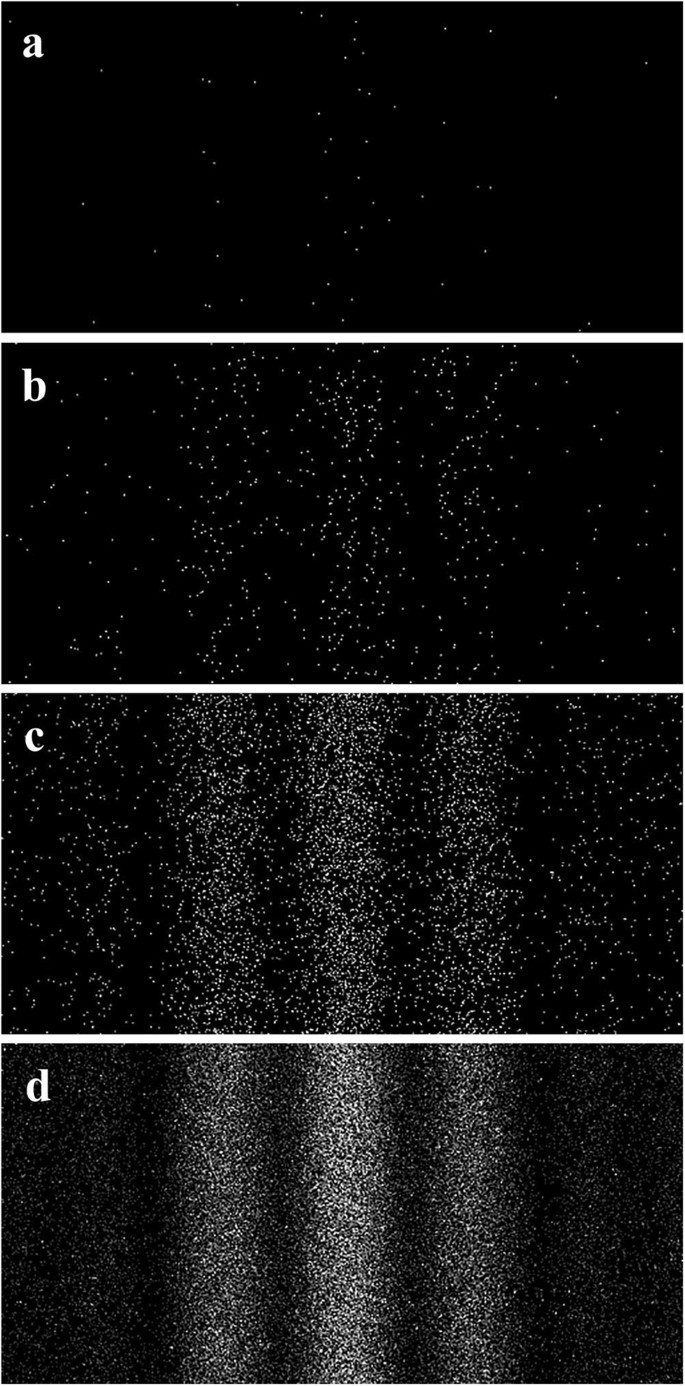
\includegraphics[width=0.14\textwidth]{Single photon double-slit}
\end{wrapfigure}
When a single photon passes through a double-slit, an interference pattern emerges. Constructive interference appears as bright bands, while destructive interference appears as dark bands. This implies the photon can pass through both slits and interfere with itself, which is a feature of classical wave.\bigskip\newline
Meanwhile, the pattern is made of individual points, indicating the particle nature of light.

\subsection*{de Broglie wavelength}
de Broglie proposed that not only photons, but all matter quanta should have wave-like properties. The de Broglie wavelength is
\begin{eqnbox}
\begin{align}
\lambda=\frac{h}{p}
\end{align}
\end{eqnbox}
The particle-like momentum $p$ and wave-like wavenumber $k=\frac{2\pi}{\l}$ are related by the de Broglie formula,
\begin{eqnbox}
\begin{align}
p=\hbar k
\end{align}
\end{eqnbox}

\section{Quantum wave function}
Born's rule is an important postulate in quantum mechanics, which states that the quantum wave function is a wave of probability amplitude. The probability density is ${\left|\psi\right|}^{2}\equiv \psi^\ast \psi$, and the probability to find the particle between $x$ and $x+dx$ is ${\left|\psi\right|}^{2}\,dx$.\bigskip\newline
The probability to find the particle in the whole space sums up to unity, so the wave function is normalized as
\begin{eqnbox}
\begin{align}
\int_{-\infty}^{\infty} {\left|\psi(x,t)\right|}^{2}\,dx=1
\end{align}
\end{eqnbox}
The expectation value of the position is
\begin{eqnbox}
\begin{align}
\langle x\rangle=\int_{-\infty}^{\infty} x{\left|\psi(x,t)\right|}^{2}\,dx
\end{align}
\end{eqnbox}
and the expectation value of the momentum is
\begin{eqnbox}
\begin{align}
\langle \hat{p}\rangle=\int_{-\infty}^{\infty} \psi^\ast(x,t)\,\hat{p}\,\psi(x, t)\,dx
\end{align}
\end{eqnbox}
where $\hat{p}=-i\hbar\frac{\p}{\p x}$ is the momentum operator. In three-dimensional space, it is generalized to $\hat{p}=-i\hbar\n$.\bigskip\newline
More generally, the expectation value of $f(x, \hat{p})$ is
\begin{eqnbox}
\begin{align}
\langle f(x, \hat{p})\rangle=\int_{-\infty}^{\infty} \psi^\ast(x,t)\,f(x, \hat{p})\,\psi(x, t)\,dx
\end{align}
\end{eqnbox}
Superposition is the key feature of wave. If wave functions $\psi_{1}$ and $\psi_{2}$ are solutions of the wave equation, then $c_{1}\psi_{1}+c_{2}\psi_{2}$ is also a solution, where $c_{1}, c_{2}\in\C$ are arbitrary complex-valued constants.

\section{Observables and measurements}
An observable is represented by an operator $\hat{O}$. The outcome of a measurement must be real number, thus we require the observable to be a Hermitian operator, i.e. $\hat{O}^\dag\equiv{(\hat{O}^\ast)}^{T}=\hat{O}$.\bigskip\newline
Some quantum states have definite value $\lambda$ of $\hat{O}$,
\begin{eqnbox}
\begin{align}
\hat{O}\psi_{\lambda}(x)=\lambda\psi_{\lambda}(x)
\end{align}
\end{eqnbox}
When we measure $\hat{O}$ on the state, we get the definite outcome $\lambda$. Examples include the position and momentum eigenstates. 

\subsection*{Position and momentum eigenstates}
A position eigenstate is given by
\begin{align}
\psi_{q}(x)=\d (x-q)\nonumber
\end{align}
and $\psi_{q}(x)$ is an eigenstate of $\hat{x}=x$,
\begin{align}
\hat{x}\psi_{q}(x)=q\psi_{q}(x)\nonumber
\end{align}
Consider a plane wave $\psi_{p}(x, t)$,
\begin{align}
\psi_{p}(x, t)=\frac{1}{\sqrt{2\pi\hbar}}e^{i\left(px-Et\right)/\hbar}\nonumber
\end{align}
we can show that the plane wave is an eigenstate of $\hat{p}=-i\hbar\frac{\p}{\p x}$,
\begin{align}
\hat{p} \psi_{p}(x, t)&=-i\hbar\frac{\p}{\p x}\frac{1}{\sqrt{2\pi\hbar}}e^{i\left(px-Et\right)/ \hbar}\nonumber\\
&=-i\hbar\cdot\frac{1}{\sqrt{2\pi\hbar}}\cdot ipe^{i\left(px-Et\right)/\hbar}\nonumber\\
&=p\psi_{p}(x, t)\nonumber
\end{align}

\subsection*{Measurement outcome of a general state}
For observables taking discrete values, the decomposition is
\begin{eqnbox}
\begin{align}
\psi(x)=\sum_{i}c_{i}\psi_{\lambda_{i}}(x)
\end{align}
\end{eqnbox}
where $\psi_{\lambda_{i}}$ is the eigenstate of $\hat{O}$ with eigenvalue $\lambda_{i}$. The probability for the measurement outcome $\lambda_{i}$ is ${\left|c_{i}\right|}^{2}$, and the wave function collapses to $\psi_{\lambda_{i}}$ after measurement.\bigskip\newline
For observables taking continuous values, the decomposition is
\begin{eqnbox}
\begin{align}
\psi(x)=\int c(\lambda)\psi_{\lambda}\,d\lambda
\end{align}
\end{eqnbox}
where $\psi_{\lambda}$ is the eigenstate of $\hat{O}$ with eigenvalue $\lambda$. The probability density for the measurement outcome $\lambda$ is ${\left|c(\lambda)\right|}^{2}$, and the wave function collapses to $\psi_{\lambda}$ after measurement.

\section{Uncertainty principle}
Uncertainty in quantum mechanics is quantified by standard deviation. Given a state, the uncertainty of the state's position and momentum are
\begin{eqnbox}
\begin{align}
\s_{x}&\equiv\sqrt{\langle x^{2}\rangle-{\langle x\rangle}^{2}}\\
\s_{p}&\equiv\sqrt{\langle \hat{p}^{2}\rangle-{\langle \hat{p}\rangle}^{2}}
\end{align}
\end{eqnbox}
For $\hat{p}=-i\hbar\frac{\p}{\p x}$, the uncertainty principle is
\begin{eqnbox}
\begin{align}
\s_{x}\s_{p}\geq \frac{\hbar}{2}
\end{align}
\end{eqnbox}

\begin{example}[Gaussian wave packet]
\label{Gaussian wave packet}
Gaussian wave packet saturates the uncertainty principle, i.e. $\s_{x}\s_{p}=\frac{\hbar}{2}$. An easy proof is given below.\bigskip\newline
We start with the wave function of the Gaussian wave packet,
\begin{eqnbox}
\begin{align}
\Psi(x,t)=\frac{1}{\sqrt{\s_{x}\sqrt{2\pi}}}e^{-x^{2}/4\s_{x}^{2}}
\end{align}
\end{eqnbox}
where $\s_{x}$ is the standard deviation of $x$.\bigskip\newline
We want to find $\langle x\rangle$, $\langle x^{2}\rangle$, $\langle \hat{p}\rangle$ and $\langle \hat{p}^{2}\rangle$.
\begin{align*}
\langle x\rangle=\int_{-\infty}^{\infty}x{\left[\frac{1}{\sqrt{\s_{x}\sqrt{2\pi}}}e^{-x^{2}/4\s_{x}^{2}}\right]}^{2} \,dx
\end{align*}
For an odd function, the integral over a symmetric interval is $0$, so $\langle x\rangle=0$.
\begin{align*}
\langle x^{2}\rangle&=\int_{-\infty}^{\infty}x^{2}{\left[\frac{1}{\sqrt{\s_{x}\sqrt{2\pi}}}e^{-x^{2}/4\s_{x}^{2}}\right]}^{2}\,dx\\
&=\frac{1}{\s_{x}\sqrt{2\pi}}\int_{-\infty}^{\infty}x^{2}e^{-x^{2}/2\s_{x}^{2}}\,dx\\
&=\frac{1}{\s_{x}\sqrt{2\pi}}\int_{-\infty}^{\infty}{\left(\frac{x}{\sqrt{2}\s_{x}}\right)}^{2}e^{-{\left(\frac{x}{\sqrt{2}\s_{x}}\right)}^{2}}\,d\left(\frac{x}{\sqrt{2}\s_{x}}\right)\cdot{\left(\sqrt{2}\s_{x}\right)}^{3}\\
&=\s_{x}^{2}
\end{align*}
It is straightforward to calculate $\langle \hat{p}\rangle$
\begin{align*}
\langle \hat{p}\rangle&=\int_{-\infty}^{\infty}\frac{1}{\sqrt{\s_{x}\sqrt{2\pi}}}e^{-x^{2}/4\s_{x}^{2}}\cdot -i\hbar\frac{\p}{\p x}\left[\frac{1}{\sqrt{\s_{x}\sqrt{2\pi}}}e^{-x^{2}/4\s_{x}^{2}}\right]\,dx\\
&=\frac{i\hbar}{\s_{x}^{3}\sqrt{2\pi}}\cdot\frac{1}{2}\int_{-\infty}^{\infty} xe^{-x^{2}/2\s_{x}^{2}}\,dx
\end{align*}
Similar to $\langle x\rangle=0$, the function being integrated is odd, so we have $\langle \hat{p}\rangle=0$.
\begin{align*}
\langle \hat{p}^{2}\rangle&=\int_{-\infty}^{\infty}\frac{1}{\sqrt{\s_{x}\sqrt{2\pi}}}e^{-x^{2}/4\s_{x}^{2}}\cdot -{\hbar}^{2}\frac{\p^2}{\p^2 x}\left[\frac{1}{\sqrt{\s_{x}\sqrt{2\pi}}}e^{-x^{2}/4\s_{x}^{2}}\right]\,dx\\
&=\frac{{\hbar}^{2}}{\s_{x}\sqrt{2\pi}}\int_{-\infty}^{\infty}e^{-x^{2}/4\s_{x}^{2}}\cdot\frac{\p}{\p x}\left[\frac{x}{2\s_{x}^{2}}e^{-x^{2}/4\s_{x}^{2}}\right]\,dx\\
&=\frac{{\hbar}^{2}}{\s_{x}^{3}\sqrt{2\pi}}\int_{-\infty}^{\infty}e^{-x^{2}/2\s_{x}^{2}}\left(\frac{1}{2}-\frac{x^{2}}{4\s_{x}^{2}}\right)\,dx
\end{align*}
To simplify the equation, we first compute the integral,
\begin{align*}
\int_{-\infty}^{\infty}e^{-x^{2}/2\s_{x}^{2}}\left(\frac{1}{2}-\frac{x^{2}}{4\s_{x}^{2}}\right)\,dx&=\int_{-\infty}^{\infty}e^{-{\left(\frac{x}{\sqrt{2}\s_{x}}\right)}^{2}}\left(\frac{1}{2}-\frac{x^{2}}{4\s_{x}^{2}}\right)\,dx\\
&=\frac{1}{2}\int_{-\infty}^{\infty}e^{-{\left(\frac{x}{\sqrt{2}\s_{x}}\right)}^{2}}\,d\left(\frac{x}{\sqrt{2}\s_{x}}\right)\cdot\sqrt{2}\s_{x}\\
&\,\,\,\,\,\,-\int_{-\infty}^{\infty}{\left(\frac{x}{\sqrt{2}\s_{x}}\right)}^{2} e^{-{\left(\frac{x}{\sqrt{2}\s_{x}}\right)}^{2}}\,d\left(\frac{x}{\sqrt{2}\s_{x}}\right)\cdot\frac{\s_{x}}{\sqrt{2}}\\
&=\frac{\sqrt{2\pi}}{4}\s_{x}
\end{align*}
After substitution,
\begin{align*}
\langle {\hat{p}}^{2}\rangle=\frac{{\hbar}^{2}}{4{\sigma_x}^{2}}
\end{align*}
Therefore, we have $\langle x\rangle=0$, $\langle x^{2}\rangle=\s_{x}^{2}$, $\langle \hat{p}\rangle=0$ and $\langle \hat{p}^{2}\rangle=\frac{\hbar^{2}}{4\s_{x}^{2}}$.
\begin{align*}
\s_{x}&=\sqrt{{\langle x^{2}\rangle}^{2}-{\langle x\rangle}^{2}}=\s_x\\
\s_{p}&=\sqrt{{\langle {\hat{p}}^{2}\rangle}^{2}-{\langle \hat{p}\rangle}^{2}}=\frac{\hbar}{2\s_x}\\
\s_{x}\s_{p}&=\s_{x}\cdot\frac{\hbar}{2\s_x}=\frac{\hbar}{2}
\end{align*}
We prove that the Gaussian wave packet saturates the uncertainty principle.
\end{example}

\section{Schr\"{o}dinger equation}
Schr\"{o}dinger equation is a linear partial differential equation that governs the evolution of a quantum system,
\begin{eqnbox}
\begin{align}
\hat{H}\psi(x, t)=i\hbar\frac{\p}{\p t}\psi(x, t)
\end{align}
\end{eqnbox}
where $\hat{H}=-\frac{\hbar^{2}}{2m}\frac{\p^{2}}{\p x^{2}}+V(x)$ is the Hamiltonian, the operator corresponding to energy.\bigskip\newline
For a state with definite energy $E$, the Schr\"{o}dinger equation is greatly simplified to the time-independent form. Substitute $\psi(x, t)=e^{-iEt/\hbar}\psi(x)$ to eq. (4.15),
\begin{align*}
\left[-\frac{\hbar^{2}}{2m}\frac{\p^{2}}{\p x^{2}}+V(x)\right]\left(e^{-iEt/\hbar}\psi(x)\right)&=i\hbar\frac{\p}{\p t}e^{-iEt/\hbar}\psi(x)\\
\left[-\frac{\hbar^{2}}{2m}\frac{d^{2}}{dx^{2}}+V(x)\right]\psi(x)\cdot e^{-iEt/\hbar}&=i\hbar\cdot-\frac{iE}{\hbar}e^{-iEt/\hbar}\psi(x)
\end{align*}
After cancellation,
\begin{eqnbox}
\begin{align}
\left[-\frac{\hbar^{2}}{2m}\frac{d^{2}}{dx^{2}}+V(x)\right]\psi(x)=E\psi(x)
\end{align}
\end{eqnbox}
This is the time-independent Schr\"{o}dinger equation.

\subsection*{A step potential problem}
\begin{wrapfigure}{r}{0\textwidth}
\hspace{-3cm}
\centering
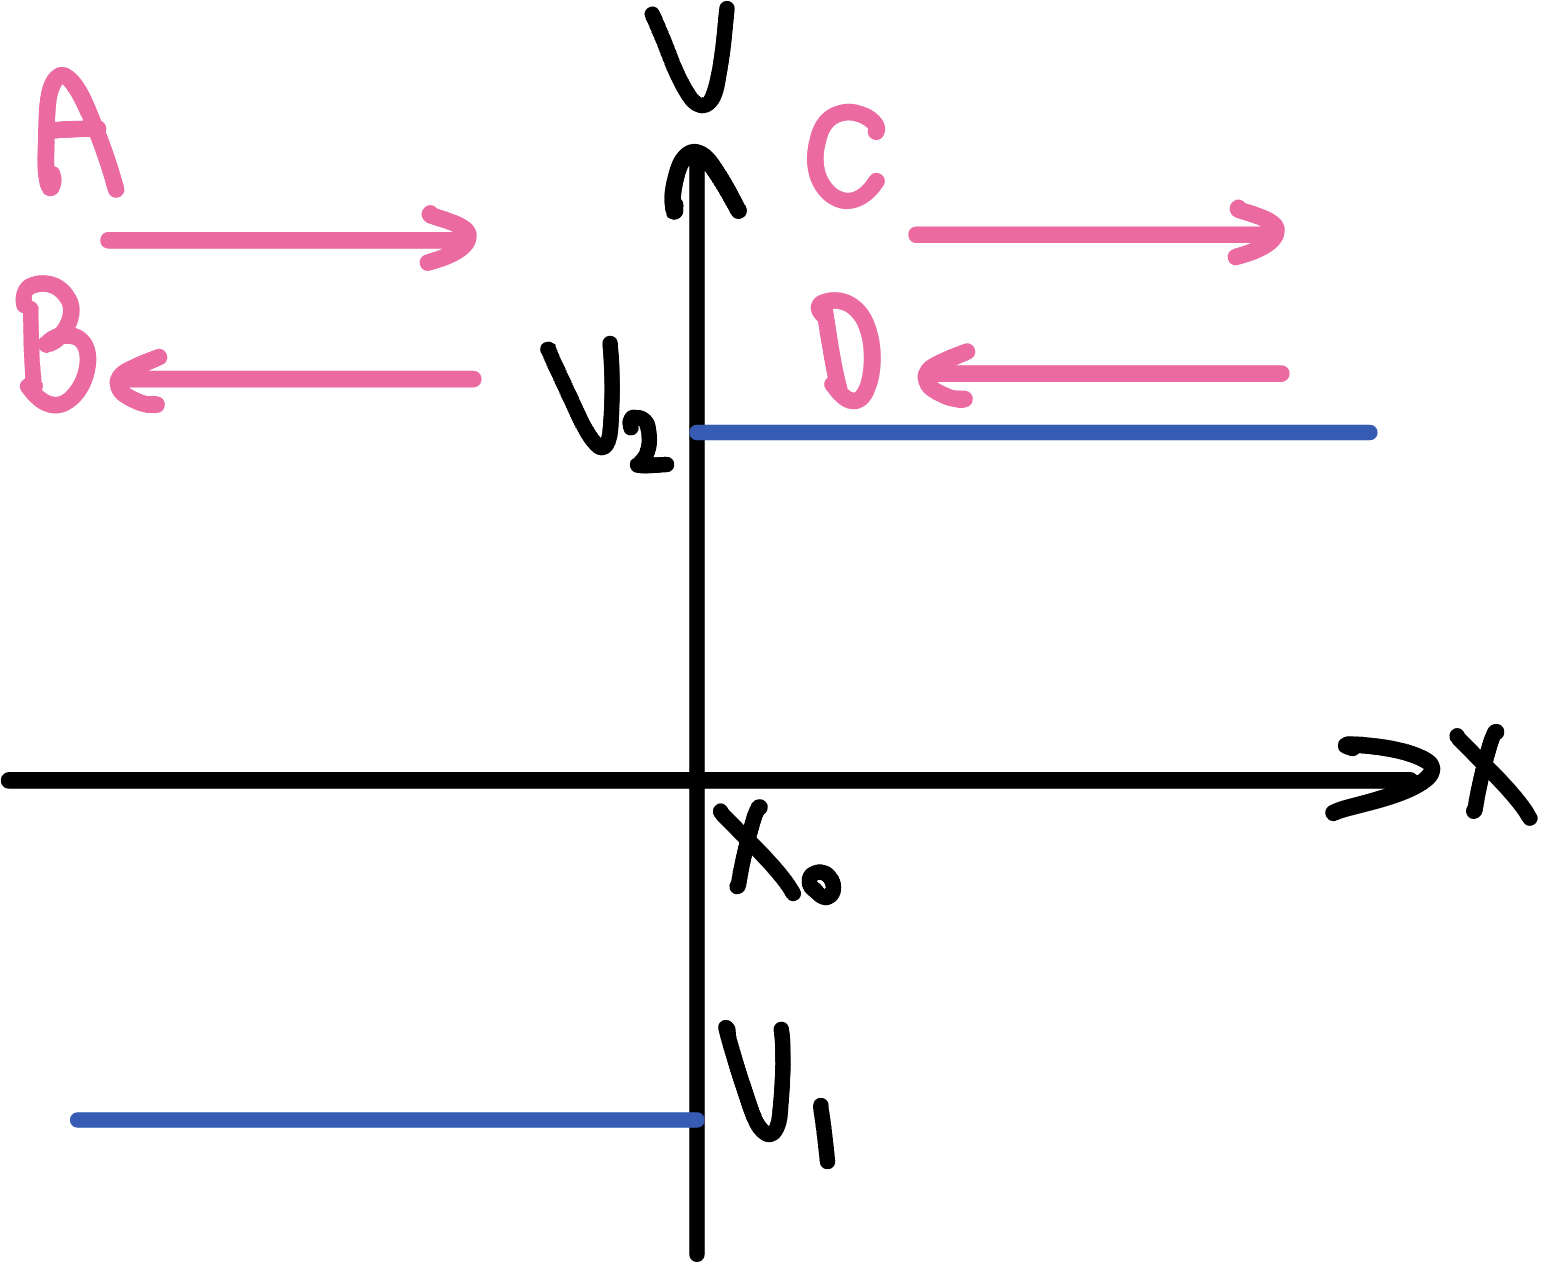
\includegraphics[width=0.3\textwidth]{A step potential problem}
\end{wrapfigure}
Consider the potential function below,
\begin{align*}
V=
\begin{cases}
V_{1}, \text{ if }x<x_{0}\\
V_{2}, \text{ if }x>x_{0}
\end{cases}
\end{align*}
and $V_{1}<V_{2}$.\bigskip\newline
Put it into eq. (4.16),
\begin{align*}
-\frac{\hbar^{2}}{2m}\frac{d^{2}}{dx^{2}}\psi(x)=(E-V)\psi(x)
\end{align*}
This is a second order linear differential equation. After rearrangement,
\begin{align*}
\frac{d^{2}}{dx^{2}}\psi(x)+\frac{2m(E-V)}{\hbar^{2}}\psi(x)=0
\end{align*}
Define $k\equiv\frac{\sqrt{2m(E-V)}}{\hbar}$, the characteristic equation is
\begin{align*}
\lambda^{2}+k^{2}\lambda&=0\\
\lambda&=\pm ik
\end{align*}
The solution of the differential equation is
\begin{eqnbox}
\begin{align}
\psi(x)=
\begin{cases}
Ae^{ik_{1}x}+Be^{-ik_{1}x}, \text{ if }x<x_{0}\\
Ce^{ik_{2}x}+De^{-ik_{2}x}, \text{ if }x>x_{0}
\end{cases}
\end{align}
\end{eqnbox}
where $k_{1}\equiv\frac{\sqrt{2m(E-V_{1})}}{\hbar}$ and $k_{2}\equiv\frac{\sqrt{2m(E-V_{2})}}{\hbar}$. $A$, $C$ denote the waves moving to the right, and $B$, $D$ denote the waves moving to the left.\bigskip\newline
We require the wave function to satisfy two continuity conditions:

\begin{itembox}
\begin{itemize}
    \item $\psi(x)$ is continuous, i.e. $\psi_{-}(x_{0})=\psi_{+}(x_{0})$. Otherwise,  $\psi'(x_{0})\to\infty$. This implies infinite momentum, since the momentum is found by using the momentum operator $\hat{p}=-i\hbar\frac{\p}{\p x}$, which consists of the first derivative.
    \item $\psi'(x)$ is continuous, i.e. $\psi_{-}'(x_{0})=\psi_{+}'(x_{0})$. Otherwise,  $\psi''(x_{0})\to\infty$. This implies infinite energy, since the energy is found by using the Hamiltonian $\hat{H}=-\frac{\hbar^{2}}{2m}\frac{\p^{2}}{\p x^{2}}+V(x)$, which consists of the second derivative.
\end{itemize}
\end{itembox}
Applying these two conditions,
\begin{eqnbox}
\begin{align}
\begin{cases}
Ae^{ik_{1}x_{0}}=\frac{k_{1}+k_{2}}{2k_{1}}Ce^{ik_{2}x_{0}}+\frac{k_{1}-k_{2}}{2k_{1}}De^{-ik_{2}x_{0}}\\
Be^{-ik_{1}x_{0}}=\frac{k_{1}-k_{2}}{2k_{1}}Ce^{ik_{2}x_{0}}+\frac{k_{1}+k_{2}}{2k_{1}}De^{-ik_{2}x_{0}}
\end{cases}
\end{align}
\end{eqnbox}
When we set $D=0$, the problem is reduced to a scattering problem. $A$ is the incoming wave, $B$ is the reflection wave, and $C$ is the transmission wave. From eq. (4.18),
\begin{eqnbox}\begin{align}
\begin{cases}
C=\frac{2k_{1}}{k_{1}+k_{2}}e^{i\left(k_{1}-k_{2}\right)x_{0}}A\\
B=\frac{k_{1}-k_{2}}{k_{1}+k_{2}}e^{2ik_{1}x_{0}}A
\end{cases}
\end{align}\end{eqnbox}

\subsection*{Quantum tunnelling}
Classically, a particle with energy $E<V_{2}$ cannot pass through the barrier $V_{2}$ and reach $x>x_{0}$. However, in the quantum case, the particle may pass through the barrier, with a probability exponentially decreasing with $x$. This phenomenon is called quantum tunnelling.\bigskip\newline
We have $k_{2}=\frac{\sqrt{2m(E-V_{2})}}{\hbar}\in\C\setminus\Q$. Define $|k_{2}|$ to be a positive real number with $k_{2}\equiv|k_{2}|i$. Using the lower part of eq. (4.17), When $x>x_{0}$,
\begin{eqnbox}\begin{align}
\psi(x)=Ce^{-\left|k_{2}\right|x}
\end{align}\end{eqnbox}
Since $e^{\left|k_{2}\right|x}\to\infty$ when $x\to\infty$, we must have $D=0$, to prevent the wave function from blowing up.
\begin{example}[$\a$-decay]
$\a$-decay is an example of quantum tunnelling. For example, the following process happens:
\begin{align*}
\prescript{238}{92}{\mathbf{U}}\to \prescript{234}{90}{\mathbf{Th}}+\prescript{4}{2}{\mathbf{He}}
\end{align*}
The $\prescript{234}{90}{\mathbf{Th}}$ part of the nuclei provides a binding potential for the $\prescript{4}{2}{\mathbf{He}}$ part, which has a small chance to escape by quantum tunnelling. The element $\prescript{238}{92}{\mathbf{U}}$ has a very long half-life of $t_{1/2}\sim4\times10^{9}\text{ years}$ because of the exponentially small decay rate.
\end{example}
\pagebreak
\subsection*{A bound state problem}
\begin{wrapfigure}{r}{0\textwidth}
\hspace{-3cm}
\centering
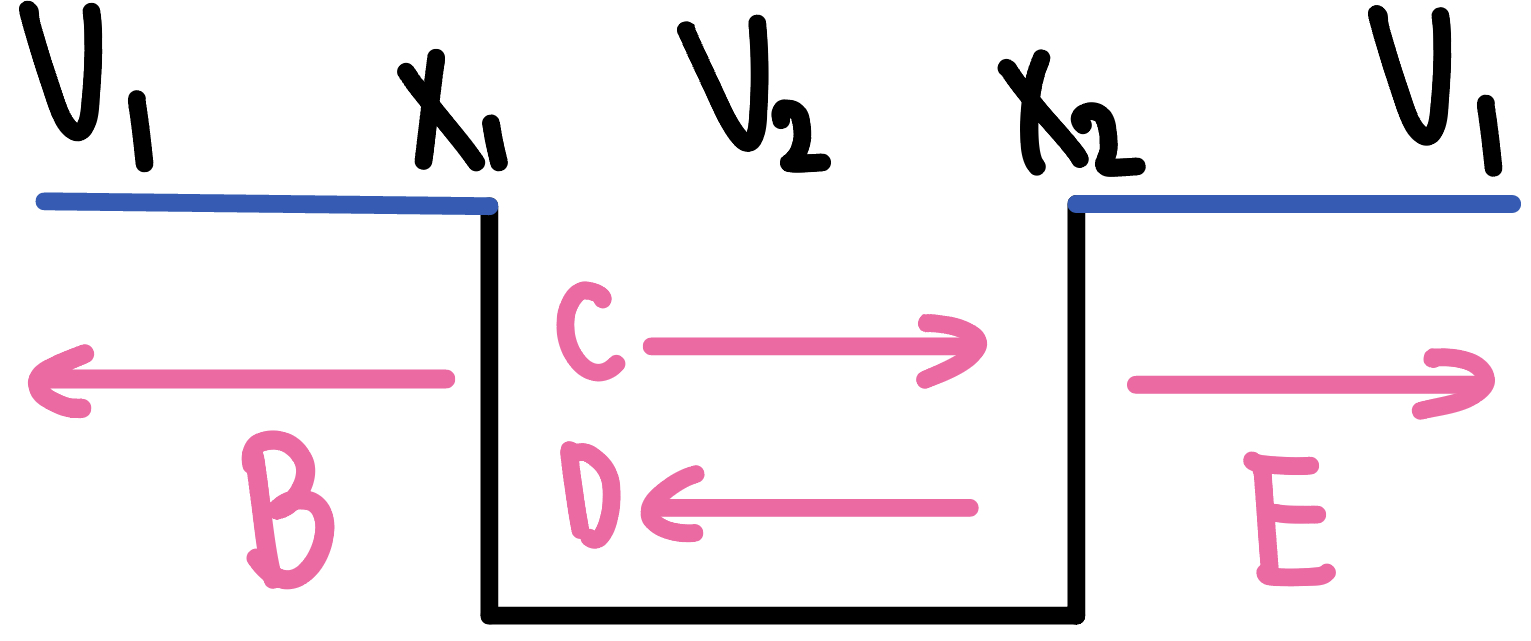
\includegraphics[width=0.3\textwidth]{A bound state problem}
\end{wrapfigure}
Consider the potential function below,
\begin{align*}
V=
\begin{cases}
V_{1},\text{ if }x>x_{1}\text{ or }x<x_{2}\\
V_{2},\text{ if }x_{1}<x<x_{2}
\end{cases}
\end{align*}
The solution of the wave function is
\begin{eqnbox}
\begin{align}
\psi(x)=
\begin{cases}
Be^{-ik_{1}x}\text{ if }x<x_{1}\\
Ce^{ik_{2}x}+De^{-ik_{2}x}, \text{ if }x_{1}<x<x_{2}\\
Ee^{ik_{1}x}\text{ if }x>x_{2}\\
\end{cases}
\end{align}
\end{eqnbox}
Similar to how we solve for the step potential problem, we apply the continuity conditions for $\psi(x)$ and $\psi'(x)$ (make sure you are familiar with the calculations).\bigskip\newline
At $x_{1}$, $\psi_{-}(x_{1})=\psi_{+}(x_{1})$,
\begin{eqnbox}
\begin{align}
Be^{-ik_{1}x_{1}}=Ce^{ik_{2}x_{1}}+De^{-ik_{2}x_{1}}
\end{align}
\end{eqnbox}
Also, $\psi'_{-}(x_{1})=\psi'_{+}(x_{1})$,
\begin{eqnbox}
\begin{align}
-ik_{1}Be^{-ik_{1}x_{1}}&=ik_{2}Ce^{ik_{2}x_{1}}-ik_{2}De^{-ik_{2}x_{1}}\nonumber\\
\implies Be^{-ik_{1}x_{1}}&=-\frac{k_{2}}{k_{1}}\cdot Ce^{ik_{2}x_{1}}+\frac{k_{2}}{k_{1}}\cdot De^{-ik_{2}x_{1}}
\end{align}
\end{eqnbox}
eq. (4.22) must be consistent with eq. (4.23),
\begin{align*}
Ce^{ik_{2}x_{1}}+De^{-ik_{2}x_{1}}=-\frac{k_{2}}{k_{1}}\cdot Ce^{ik_{2}x_{1}}+\frac{k_{2}}{k_{1}}\cdot De^{-ik_{2}x_{1}}
\end{align*}
After simplification,
\begin{eqnbox}
\begin{align}
\frac{C}{D}=\frac{k_{2}-k_{1}}{k_{2}+k_{1}}e^{-2ik_{2}x_{1}}
\end{align}
\end{eqnbox}
At $x_{2}$, $\psi_{-}(x_{2})=\psi_{+}(x_{2})$,
\begin{eqnbox}
\begin{align}
Ee^{ik_{1}x_{2}}=Ce^{ik_{2}x_{2}}+De^{-ik_{2}x_{2}}
\end{align}
\end{eqnbox}
\pagebreak
Also, $\psi'_{-}(x_{2})=\psi'_{+}(x_{2})$,
\begin{eqnbox}
\begin{align}
ik_{1}Ee^{ik_{1}x_{2}}&=ik_{2}Ce^{ik_{2}x_{2}}-ik_{2}De^{-ik_{2}x_{2}}\nonumber\\
\implies Ee^{ik_{1}x_{2}}&=\frac{k_{2}}{k_{1}}\cdot Ce^{ik_{2}x_{2}}-\frac{k_{2}}{k_{1}}\cdot De^{-ik_{2}x_{2}}
\end{align}
\end{eqnbox}
We notice that eq. (4.25), eq.(4.26) are very similar to eq. (4.22), eq. (4.23). By comparing these equations, we can get an equation analogous to eq. (4.24) by doing the replacement $k_{1}\to-k_{1}$ and $x_{1}\leftrightarrow x_{2}$,
\begin{eqnbox}
\begin{align}
\frac{C}{D}=\frac{k_{2}+k_{1}}{k_{2}-k_{1}}e^{-2ik_{2}x_{2}}
\end{align}
\end{eqnbox}
eq. (4.24) and eq. (4.27) are consistent with each other. After combining them,
\begin{eqnbox}
\begin{align}
e^{2ik_{2}(x_{2}-x_{1})}={\left(\frac{k_{2}+k_{1}}{k_{2}-k_{1}}\right)}^{2}
\end{align}
\end{eqnbox}
Recall that $k_{1}\equiv\frac{\sqrt{2m(E-V_{1})}}{\hbar}$ and $k_{2}\equiv\frac{\sqrt{2m(E-V_{2})}}{\hbar}$, eq. (4.28) allows us to solve for the energy $E$. The energy takes a series of discrete values until $E>V_{2}$, after which there is a continuous spectrum.

\subsection*{Infinite potential well}
Take the limit $V_{1}\to\infty$, keep $E$ and $V_{2}$ fixed, we have an infinite potential well. Since $k_{1}\to i\infty$, we have $\psi(x)=0$ at $x<x_{1}$ or $x>x_{2}$, i.e. the probability to find the particle being outside the potential well is zero.\bigskip\newline
From eq. (4.28),
\begin{align*}
e^{2ik_{2}(x_{2}-x_{1})}&=1\\
k_{2}(x_{2}-x_{1})&=n\pi, n\in\N\\
\frac{\sqrt{2m(E_{n}-V_{2})}}{\hbar}(x_{2}-x_{1})&=n\pi
\end{align*}
After solving,
\begin{eqnbox}
\begin{align}
E_{n}=\frac{n^{2}\pi^{2}\hbar^{2}}{2m{(x_{2}-x_{1})}^{2}}+V_{2}
\end{align}
\end{eqnbox}
We start with one particle in the system, so we cannot take $n=0$, which just means $\psi(x)=0$. The bound states in the infinite potential well have discrete energy levels.\bigskip\newline
At $x_{1}<x<x_{2}$,
\begin{eqnbox}
\begin{align}
\psi(x)&=Ce^{ik_{2}x}+De^{-ik_{2}x}\nonumber\\
&=Ce^{ik_{2}x}-Ce^{2ik_{2}x_{1}}\cdot e^{-ik_{2}x}\nonumber\\
&=Ce^{ik_{2}x_{1}}\left[e^{ik_{2}(x-x_{1})-e^{ik_{2}(x_{1}-x)}}\right]\nonumber\\
&=2iCe^{ik_{2}x_{1}}\left[\frac{e^{ik_{2}(x-x_{1})}-e^{-ik_{2}(x-x_{1})}}{2i}\right]\nonumber\\
&=2iCe^{ik_{2}x_{1}}\sin\left[k_{2}(x-x_{1})\right]\nonumber\\
&=2iCe^{ik_{2}x_{1}}\sin\left[n\pi\left(\frac{x-x_{1}}{x_{2}-x_{1}}\right)\right]\nonumber\\
\implies \psi(x)&\propto \sin\left[n\pi\left(\frac{x-x_{1}}{x_{2}-x_{1}}\right)\right]
\end{align}
\end{eqnbox}
You may have spotted something weird about the infinite potential well. Outside the potential well, we have $\psi'(x)=0$ everywhere, but inside the well, we find $\psi'(x_{1}), \psi'(x_{2})\neq0$. This means the continuity condition of the first derivative of the wave function breaks down at the boundary.\bigskip\newline
Such observation is indeed correct. The infinite potential well is not a physically realistic system, since there is no known physical mechanism that generates an infinitely deep potential well. Despite this, the infinite potential well is still useful as a simplified model of some real-life problems, e.g. a particle confined in a very deep finite potential well.

\section{Identical particles}
Consider two identical particles. If $\psi(x_{1}, x_{2}, t)$ is a solution to the Schr\"{o}dinger equation, then $\psi(x_{2}, x_{1}, t)$ must also does.\bigskip\newline
There are two kinds of multi-particle wave functions that satisfy the identical particle postulate.
\begin{itembox}
\begin{itemize}
    \item Symmetric wave function with $\psi(x_{1}, x_{2}, t)=\psi(x_{2}, x_{1}, t)$. The particles described by such wave functions are bosons. For fundamental particles, bosons represent the forces of nature, e.g. photons and gravitons.
    \item Anti-symmetric wave function with $\psi(x_{1}, x_{2}, t)=-\psi(x_{2}, x_{1}, t)$. The particles described by such wave functions are fermions. For fundamental particles, fermions represent the building block of matter, e.g. electrons and quarks.
\end{itemize}
\end{itembox}
When occupying quantum states, fermions obey a special rule, known as the Pauli's exclusion principle.
\begin{theorem}[Pauli's exclusion principle]
Two or more identical fermions cannot occupy the same quantum state.\bigskip\newline
If two fermions occupy the same state, $\psi(x_{1}, x_{2}, t)=\psi(x_{2}, x_{1}, t)$. Considering the definition of fermions, $\psi(x_{1}, x_{2}, t)=-\psi(x_{2}, x_{1}, t)$, this means $\psi(x_{1}, x_{2}, t)=0$, so such system does not exist.
\end{theorem}
An energy level is a concept different from a quantum state. Two fermions can occupy the same energy level. For example, two electrons in a hydrogen atom can occupy the same energy level, but having different spin, so that they still occupy two different quantum states.

\addcontentsline{toc}{section}{Problems}
\section*{Problems}
\begin{problem}
Show that the Gaussian wave packet saturates the uncertainty principle (the purpose of this problem is forcing you to do the tedious calculation once).
\end{problem}

\begin{solbox}
The derivation is given in the notes, see \hyperref[Gaussian wave packet]{Example 4.1 - Gaussian wave packet}.
\end{solbox}

\begin{problem}
Consider a wave packet moving towards a narrow barrier located at $x=0$, with the incoming energy lower than the height of the barrier.
\begin{figure}[H]
\centering
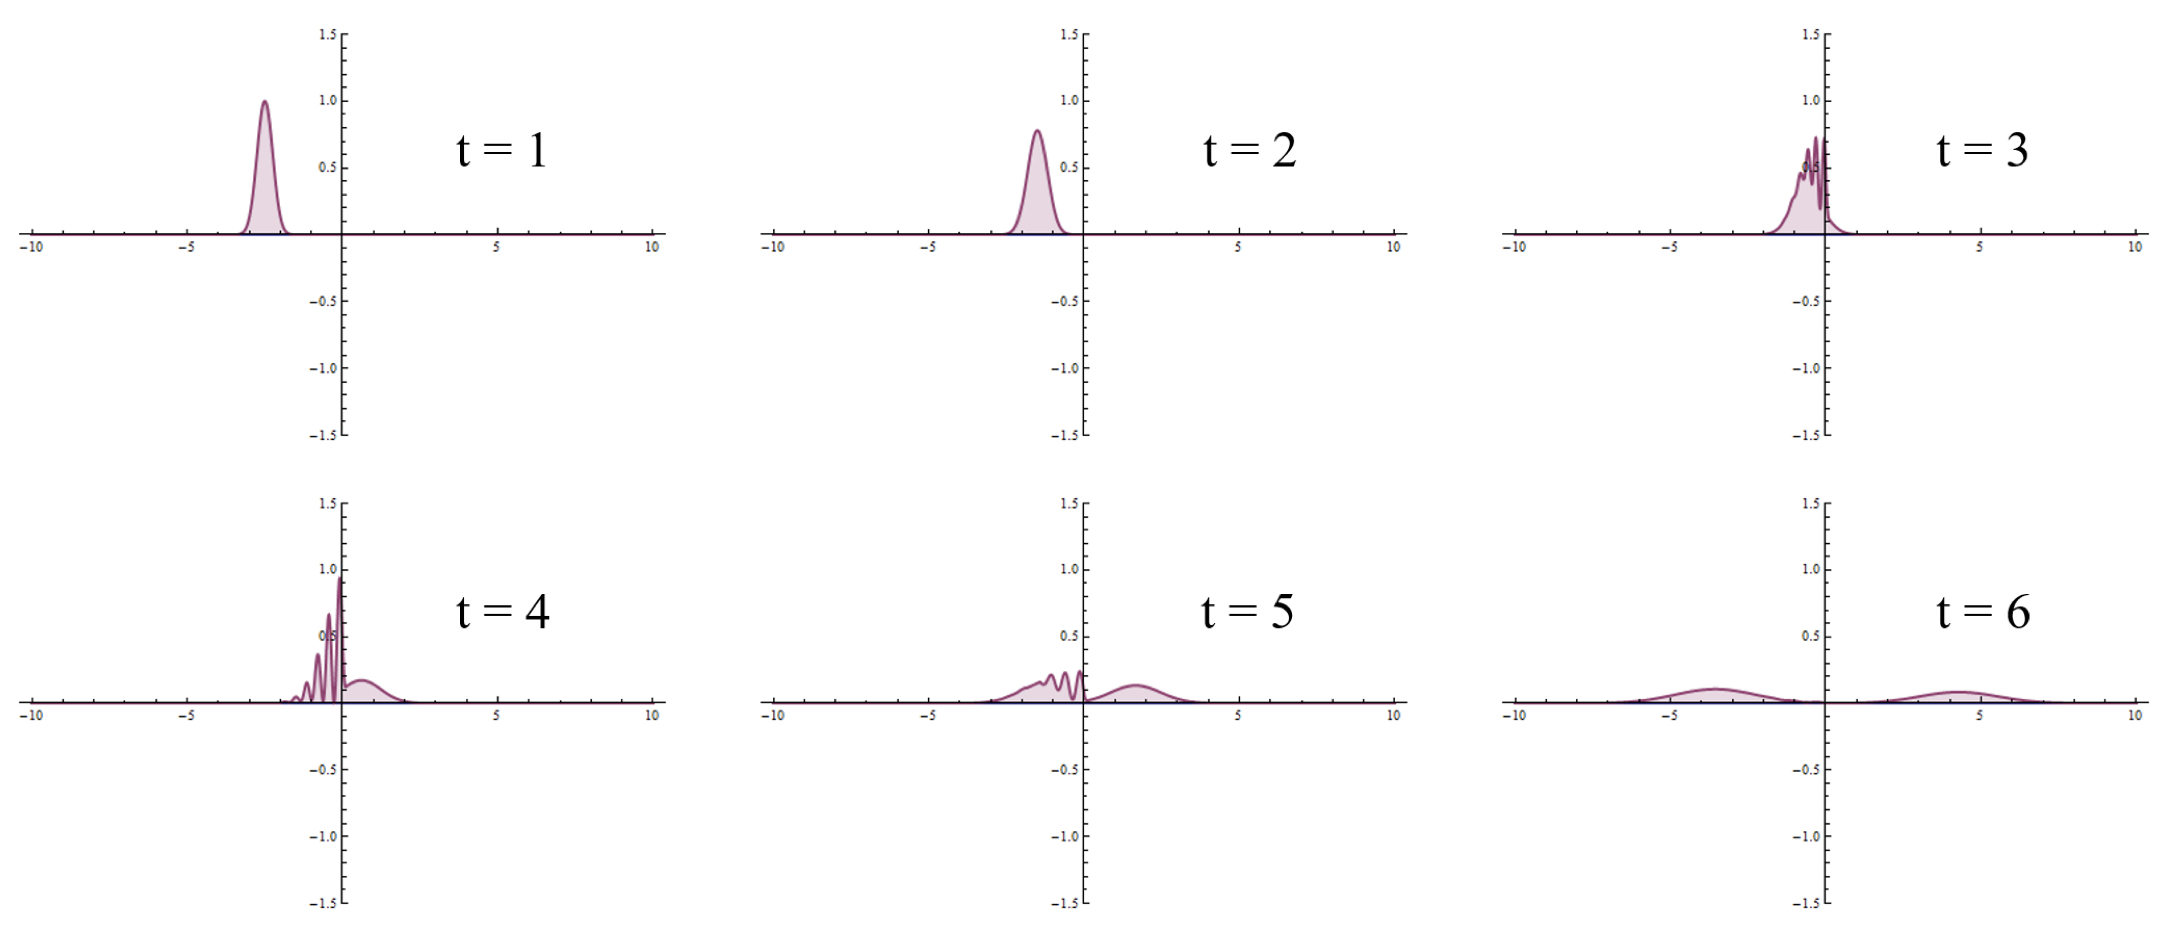
\includegraphics[width=\textwidth]{Scattering of a wave packet}
\end{figure}
\noindent a) Why is the spread of the wave packet wider at $t=2$ compared to $t=1$?\bigskip\newline
b) Why is the wave packet lower at $t=2$ compared to $t=1$?\bigskip\newline
c) Qualitatively explain the ripples observed at $t=3, 4\text{ and }5$.
\end{problem}

\begin{solbox}
a) Wave packet spreads due to a superposition with multiple momenta and thus multiple speeds.\bigskip\newline
b) The wave packet has become wider at $t=2$, so it becomes lower to preserve probability, i.e. $\int_{-\infty}^{\infty}{\left|\psi(x)\right|}^{2}\,dx=1$ at any time.\bigskip\newline
c) Ripples are formed by the interference between incoming wave and reflection wave.
\end{solbox}

\subsection*{2019-20 Fall Final Q3 - Infinite potential well}
A particle with mass $m$ is inside an infinite potential well with width $L$, as illustrated in potential (i) below. The bottom of the well has potential energy $V=0$ for $0<x<L$.
\begin{figure}[H]
\centering
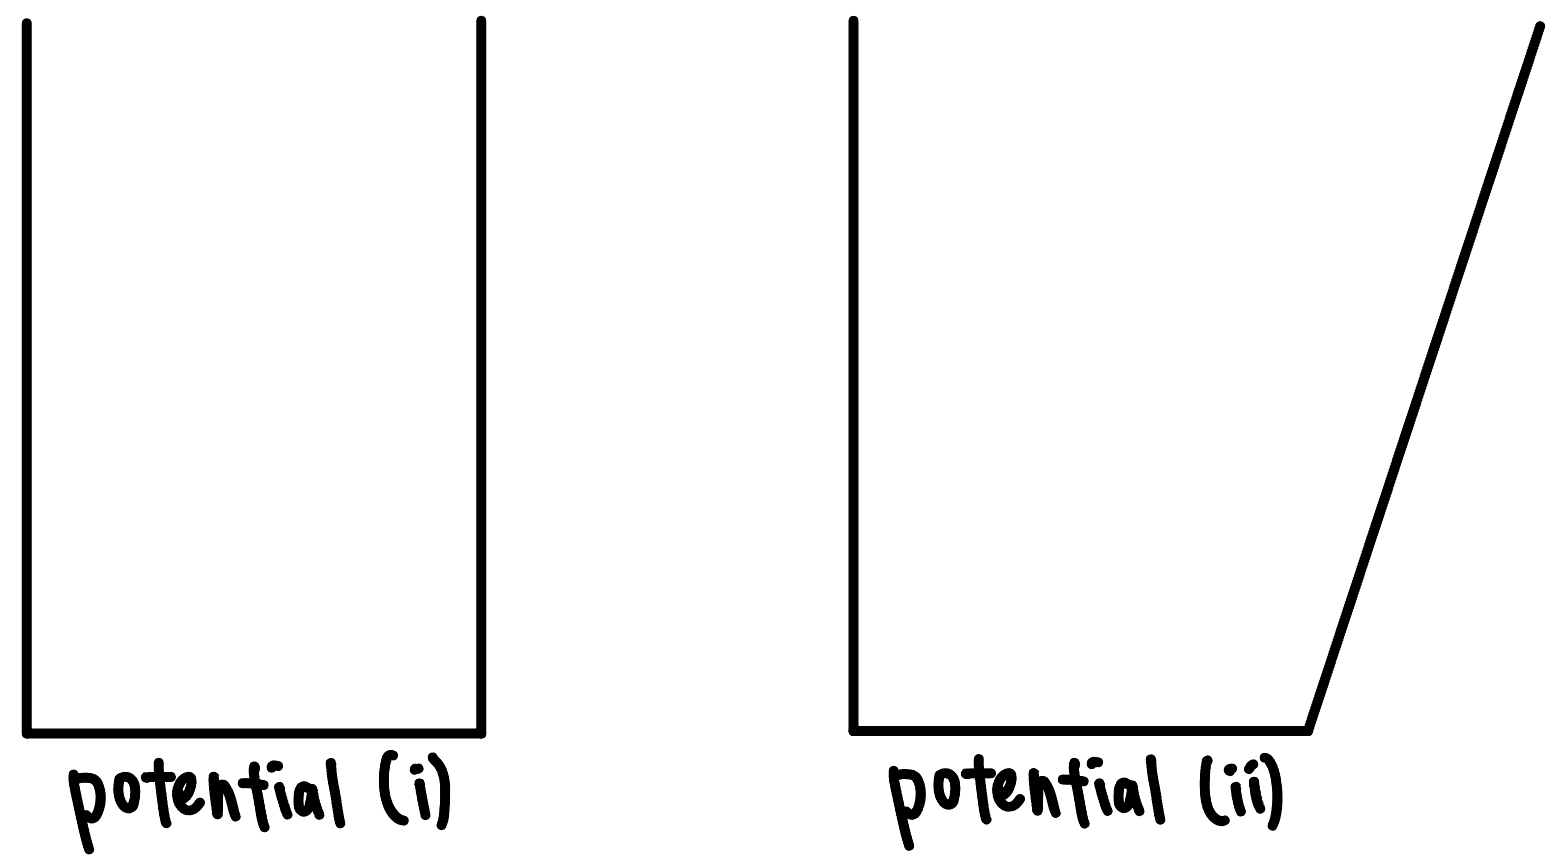
\includegraphics[width=0.6\textwidth]{Infinite potential well}
\end{figure}
\noindent a) Write down the wave function of possible states (with proper normalization).\bigskip\newline
b) Compute the energy of these states. Draw the energy of the first three states as horizontal lines on the above figure.\bigskip\newline
c) For the lowest energy state, compute the uncertainty $\s_{x}$ and $\s_{p}$. Verify that the uncertainty principle is satisfied.\bigskip\newline
d) If the shape of the potential is changed into potential (ii) shown above, qualitatively draw the energy of the first three states on the above figure.

\begin{solbox}
a) Using eq. (4.30),
\begin{align*}
\psi(x)\propto\sin\left(\frac{n\pi x}{L}\right)=A\sin\left(\frac{n\pi x}{L}\right)
\end{align*}
where $A$ is a normalization constant. Using the normalization condition,
\begin{align*}
\int_{0}^{L}{\left|\psi(x)\right|}^{2}\,dx&=1\\
\int_{0}^{L}A^{2}\sin^{2}\left(\frac{n\pi x}{L}\right)\,dx&=1\\
A&=\sqrt{\frac{2}{L}}
\end{align*}
Therefore, $\psi(x)=\sqrt{\frac{2}{L}}\sin\left(\frac{n\pi x}{L}\right)$.\bigskip\newline
This problem can also be solved by directly solving the time-independent Schr\"{o}dinger equation. For $0<x<L$, we substitute $V(x)=0$,
\begin{align*}
-\frac{\hbar^{2}}{2m}\frac{d^{2}}{dx^{2}}\psi(x)&=E\psi(x)
\end{align*}
After rearrangement,
\begin{align*}
\frac{d^{2}}{dx^{2}}\psi(x)+k^{2}\psi(x)=0
\end{align*}
where $k\equiv\frac{\sqrt{2mE}}{\hbar}$. Solving the differential equation,
\begin{align*}
\psi(x)=A\sin(kx)+B\cos(kx)
\end{align*}
where $A$ and $B$ are constants to be determined. Outside the potential well, we have $\psi(x)=0$. To satisfy the continuity conditions of the wave function, we must have $\psi(0)=\psi(L)=0$. 
\begin{align*}
\psi(0)&=B=0\implies B=0\\
\psi(L)&=A\sin(kL)=0\implies k=\frac{n\pi}{L}, n\in\N
\end{align*}
Therefore, $\psi(x)=A\sin\left(\frac{n\pi x}{L}\right)$. $A$ is determined by the normalization condition as shown above.\bigskip\newline
b) and d)
\begin{align*}
E_{n}=\frac{n^{2}\pi^{2}\hbar^{2}}{2mL^{2}}
\end{align*}
The energy levels in potential (ii) are lower than those in potential (i).
\begin{figure}[H]
\centering
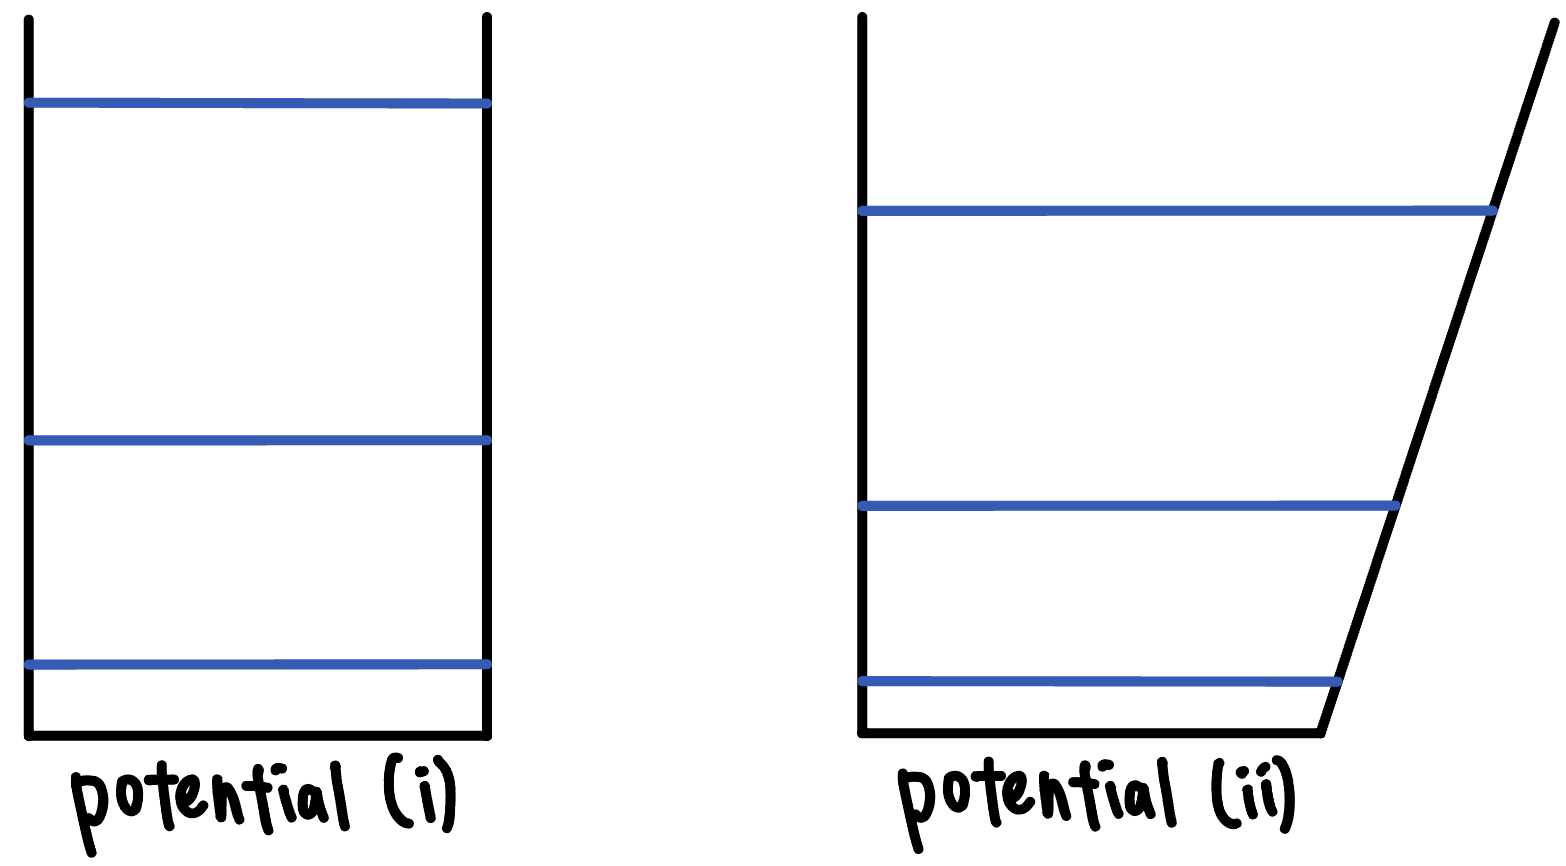
\includegraphics[width=0.6\textwidth]{Infinite potential well energy levels}
\caption{The first three energy levels of potential (i) and (ii)}
\end{figure}
\noindent
c) The ground state is $n=1$. We want to find $\langle x\rangle$, $\langle x^{2}\rangle$, $\langle \hat{p}\rangle$ and $\langle \hat{p}^{2}\rangle$.
\begin{align*}
\langle x\rangle&=\frac{L}{2}\\
\langle x^{2}\rangle&=\int_{0}^{L}x^{2}{\left|\psi(x)\right|}^{2}\,dx\\
&=\frac{2}{L}\int_{0}^{L}x^{2}\sin^{2}\left(\frac{\pi x}{L}\right)\,dx
\end{align*}
Substitute $z=\frac{x}{L}$,
\begin{align*}
\frac{2}{L}\int_{0}^{L}x^{2}\sin^{2}\left(\frac{\pi x}{L}\right)\,dx&=2L^{2}\int_{0}^{1}z^{2}\sin^{2}\left(\pi z\right)\,dz\\
&=2L^{2}\left(\frac{1}{6}-\frac{1}{4\pi^{2}}\right)\\
&=L^{2}\left(\frac{1}{3}-\frac{1}{2\pi^{2}}\right)
\end{align*}
Since the wave function is a standing wave in potential (i), $\langle \hat{p}\rangle=0$.
\begin{align*}
\frac{\langle \hat{p}^{2}\rangle}{2m}&=E_{1}\\
\langle \hat{p}^{2}\rangle&=\frac{\pi^{2}\hbar^{2}}{2mL^{2}}\cdot2m\\
&=\frac{\pi^{2}\hbar^{2}}{L^{2}}
\end{align*}
Therefore,
\begin{align*}
\s_{x}&=\sqrt{\langle x^{2}\rangle-{\langle x\rangle}^{2}}\\
&=L\sqrt{\frac{1}{12}-\frac{1}{2\pi^{2}}}\\
\s_{p}&=\sqrt{\langle \hat{p}^{2}\rangle-{\langle \hat{p}\rangle}^{2}}\\
&=\frac{\pi\hbar}{L}\\
\s_{x}\s_{p}&=\pi\hbar\sqrt{\frac{1}{12}-\frac{1}{2\pi^{2}}}\\
&>\frac{\hbar}{2}
\end{align*}
The uncertainty principle is satisfied.
\end{solbox}

\subsection*{2020-21 Fall Final Q2 - Estimation of photons}
Consider a beam of light with wavelength $500\text{nm}$ and total energy $1\text{J}$. Estimate the number of photons and total momentum of this beam of light (assuming the photons are moving in the same direction).

\begin{solbox}
Let $N$ be the total number of photons.
\begin{align*}
N\cdot \frac{hc}{\l}&=E\\
N&=\frac{E\l}{hc}\\
&=2.52\times10^{18}
\end{align*}
For particles with zero rest mass, we have $E=pc$, so
\begin{align*}
p&=\frac{E}{c}\\
&=3.33\times10^{-9}\text{kg}\text{m}\text{s}^{-1}
\end{align*}
\end{solbox}

\subsection*{2020-21 Fall Final Q4 - Scattering and bound states}
A finite potential well with width $L$ is shown below. The bottom of the well has potential energy $V=0$, while the two ends have height $V_{1}$ and $V_{2}$ respectively. A particle with mass $m$ and energy $\e$ is inside this potential well.
\begin{figure}[H]
\centering
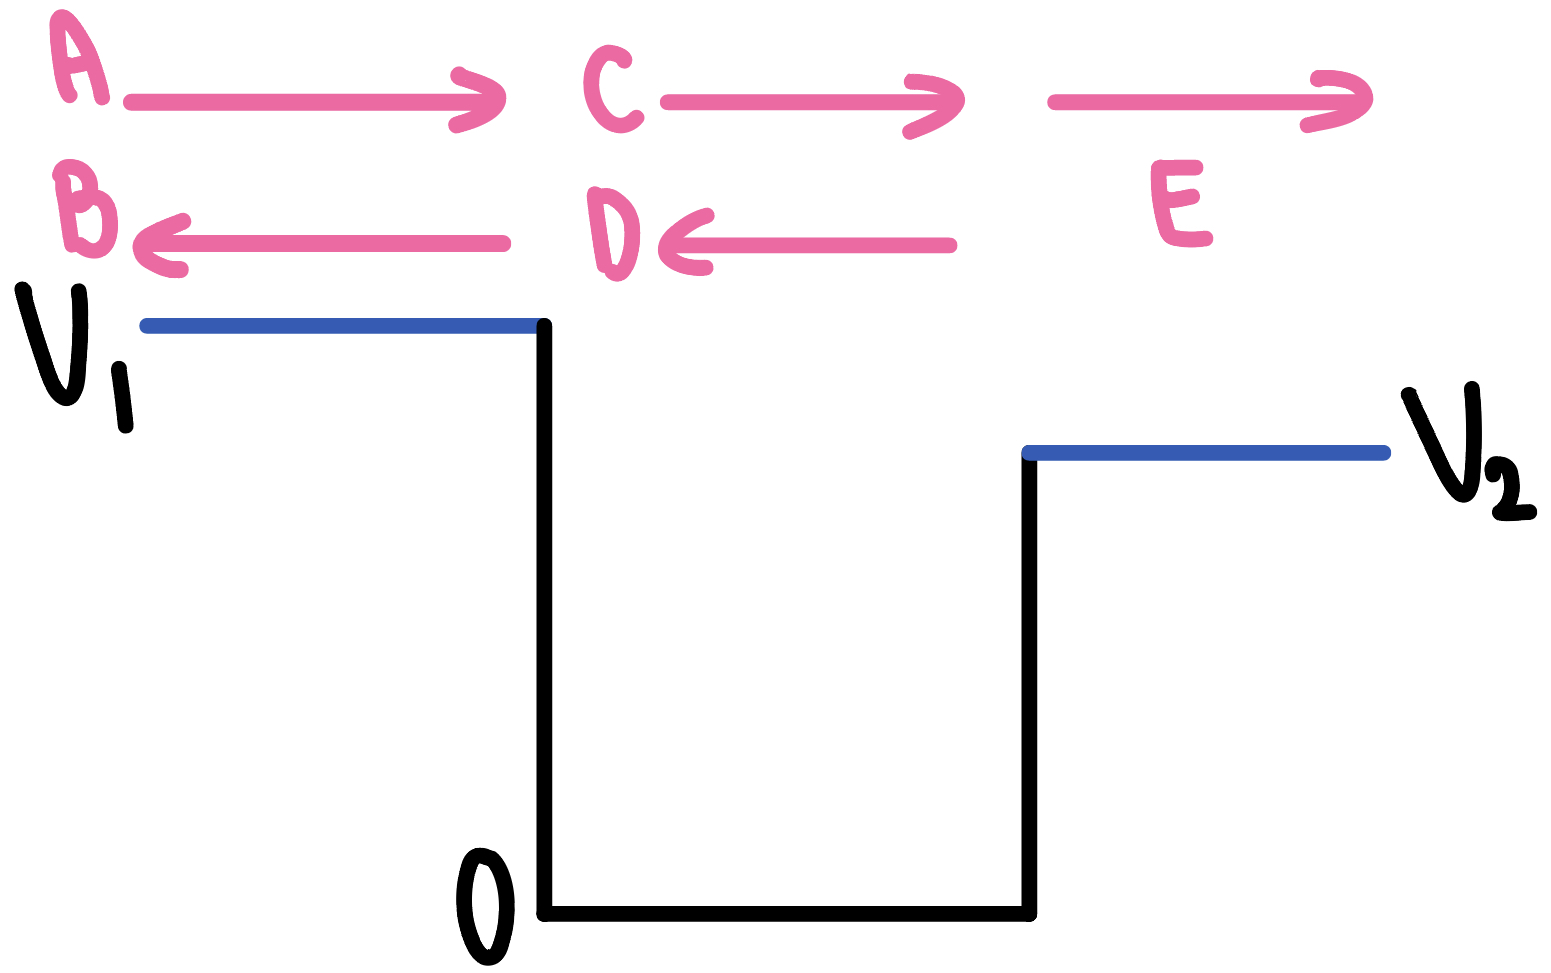
\includegraphics[width=0.4\textwidth]{Scattering and bound states}
\end{figure}
\noindent a) For the scattering problem above, calculate the relation between $A$ and $B$.\bigskip\newline
b) For the bound state problem $A=0$, calculate the condition for bound state to exist.

\begin{solbox}
a) The potential function is
\begin{align*}
V(x)=
\begin{cases}
V_{1}\text{ if }x<0\\
0\text{ if }0<x<L\\
V_{2}\text{ if }x>L
\end{cases}
\end{align*}
We start with the time-independent Schr\"{o}dinger equation,
\begin{align*}
\left[-\frac{\hbar^{2}}{2m}\frac{d^{2}}{dx^{2}}+V(x)\right]\psi(x)=\e\psi(x)
\end{align*}
After rearrangement,
\begin{align*}
\frac{d^{2}}{dx^{2}}\psi(x)+k^{2}(x)\psi(x)=0
\end{align*}
where $k(x)\equiv\frac{\sqrt{2m(\e-V(x))}}{\hbar}$.\bigskip\newline
The solution of the wave function is
\begin{align*}
\psi(x)=
\begin{cases}
Ae^{ik_{1}x}+Be^{-ik_{1}x}\text{ if }x<0\\
Ce^{ik_{0}x}+De^{-ik_{0}x}\text{ if }0<x<L\\
Ee^{ik_{2}x}\text{ if }x>L
\end{cases}
\end{align*}
where $k_{1}\equiv\frac{\sqrt{2m(\e-V_{1})}}{\hbar}$, $k_{0}\equiv\frac{\sqrt{2m\e}}{\hbar}$ and $k_{2}\equiv\frac{\sqrt{2m(\e-V_{2})}}{\hbar}$.\bigskip\newline
By the continuity conditions at $x=0$,
\begin{align*}
\psi_{-}(0)&=\psi_{+}(0)\implies A+B=C+D\\
\psi'_{-}(0)&=\psi'_{+}(0)\implies k_{1}(A-B)=k_{0}(C-D)
\end{align*}
Similarly, by the continuity conditions at $x=L$,
\begin{align*}
\psi_{-}(L)&=\psi_{+}(L)\implies Ce^{ik_{0}L}+De^{-ik_{0}L}=Ee^{ik_{2}L}\\
\psi'_{-}(L)&=\psi'_{+}(L)\implies k_{0}\left(Ce^{ik_{0}L}-De^{-ik_{0}L}\right)=k_{2}E^{ik_{2}L}
\end{align*}
We can get our desired result by solving these four equations, and the process is quite tedious.\bigskip\newline
Solving the first two equations, we get
\begin{align*}
A&=\frac{k_{1}+k_{0}}{2k_{1}}C+\frac{k_{1}-k_{0}}{2k_{1}}D\\
B&=\frac{k_{1}-k_{0}}{2k_{1}}C+\frac{k_{1}+k_{0}}{2k_{1}}D\\
\implies \frac{B}{A}&=\frac{(k_{1}-k_{0})C+(k_{1}+k_{0})D}{(k_{1}+k_{0})C+(k_{1}-k_{0})D}
\end{align*}
Solving the last two equations, we get
\begin{align*}
Ce^{ik_{0}L}&=\frac{k_{0}+k_{2}}{2k_{0}}Ee^{ik_{2}L}\\
De^{-ik_{0}L}&=\frac{k_{0}-k_{2}}{2k_{0}}Ee^{ik_{2}L}\\
\frac{C}{D}&=\frac{k_{0}+k_{2}}{k_{0}-k_{2}}e^{-2ik_{0}L}\\
\implies D&=\frac{k_{0}-k_{2}}{k_{0}+k_{2}}Ce^{2ik_{0}L}
\end{align*}
Substituting the relation between $C$ and $D$ into $\frac{B}{A}$,
\begin{align*}
\frac{B}{A}&=\frac{(k_{1}-k_{0})+\left(\frac{k_{0}-k_{2}}{k_{0}+k_{2}}\right)(k_{1}+k_{0})e^{2ik_{0}L}}{(k_{1}+k_{0})+\left(\frac{k_{0}-k_{2}}{k_{0}+k_{2}}\right)(k_{1}-k_{0})e^{2ik_{0}L}}\\
&=\frac{(k_{1}-k_{0})(k_{2}+k_{0})-(k_{1}+k_{0})(k_{2}-k_{0})e^{2ik_{0}L}}{(k_{1}+k_{0})(k_{2}+k_{0})-(k_{1}-k_{0})(k_{2}-k_{0})e^{2ik_{0}L}}
\end{align*}
b) For bound state to exist, we require $0<\e\leq V_{2}\leq V_{1}$, so the particle has insufficient energy to escape from the potential well. This implies $k_{1}\equiv\frac{\sqrt{2m(\e-V_{1})}}{\hbar}$ is imaginary.\bigskip\newline
Since $e^{ik_{1}x}\to\infty$ when $x\to-\infty$, we must have $A=0$, to prevent the wave function from blowing up. Using (a),
\begin{align*}
A=\frac{(k_{1}+k_{0})(k_{2}+k_{0})-(k_{1}-k_{0})(k_{2}-k_{0})e^{2ik_{0}L}}{(k_{1}-k_{0})(k_{2}+k_{0})-(k_{1}+k_{0})(k_{2}-k_{0})e^{2ik_{0}L}}B
\end{align*}
Since $A=0$,
\begin{align}
(k_{1}+k_{0})(k_{2}+k_{0})-(k_{1}-k_{0})(k_{2}-k_{0})e^{2ik_{0}L}&=0\nonumber\\
\frac{(k_{1}+k_{0})(k_{2}+k_{0})}{(k_{1}-k_{0})(k_{2}-k_{0})}&=e^{2ik_{0}L}
\end{align}
Recall that $k_{1}\equiv\frac{\sqrt{2m(\e-V_{1})}}{\hbar}$, $k_{0}\equiv\frac{\sqrt{2m\e}}{\hbar}$ and $k_{2}\equiv\frac{\sqrt{2m(\e-V_{2})}}{\hbar}$,
\begin{align}
\frac{\left(1+i\sqrt{\frac{V_{1}}{\e}-1}\right)\left(1+i\sqrt{\frac{V_{2}}{\e}-1}\right)}{\left(1-i\sqrt{\frac{V_{1}}{\e}-1}\right)\left(1-i\sqrt{\frac{V_{2}}{\e}-1}\right)}=e^{\frac{2\sqrt{2m\e}}{\hbar}Li}
\end{align}
eq. (4.32) is a relation on $\e$, $V_{1}$ and $V_{2}$. Bound state exists only if there exists a solution $\e\in(0, V_{2}]$ to eq. (4.32) (answering up to eq. (4.31) is sufficient to get full mark).
\end{solbox}

\subsection*{2022-23 Fall Final Q2 - Quantum particle in an infinite well}
Consider a particle with mass $m$ and definite total energy $E$ in the following potential: when $x<-L$ or $x>L$, the potential is infinitely high; when $-L<x<0$, the potential is $0$; and when $0<x<L$, the height of the potential is $V$.\bigskip\newline
Let the wave function be $\psi_{-}=d_{-}\cos{\left[k_{-}(x+L)\right]}+c_{-}\sin{\left[k_{-}(x+L)\right]}$ when $-L<x<0$ and $\psi_{+}=d_{+}\cos{\left[k_{+}(x-L)\right]}+c_{+}\sin{\left[k_{+}(x-L)\right]}$ when $0<x<L$.\bigskip\newline
a) Find the expressions of $k_{-}$ and $k_{+}$.\bigskip\newline
b) Find the ratios $\frac{d_{-}}{c_{-}}$ and $\frac{d_{+}}{c_{+}}$.\bigskip\newline
c) Find the two conditions for the wave functions $\psi_{-}$ and $\psi_{+}$ to be consistent at $x=0$.\bigskip\newline
d) In the limit $V\to0$, solve the two conditions in part (c) directly, find all the bound states and write down their energies. Key steps of the solution should be provided.\bigskip\newline
e) Compare your solution in part (d) with a simple infinite potential well. Are they the same? (Yes or no, no reason needs to be provided).\bigskip\newline
f) If $V$ is small but non-zero, Taylor expand $V$ to the linear order and find all bound state energies.

\begin{solbox}
a) The potential function is
\begin{align*}
V(x)=
\begin{cases}
0\text{ if }-L<x<0\\
V\text{ if }0<x<L
\end{cases}
\end{align*}
We start with the time-independent Schr\"{o}dinger equation,
\begin{align*}
\left[-\frac{\hbar^{2}}{2m}\frac{d^{2}}{dx^{2}}+V(x)\right]\psi(x)=E\psi(x)
\end{align*}
After rearrangement,
\begin{align*}
\frac{d^{2}}{dx^{2}}\psi(x)+k^{2}(x)\psi(x)=0
\end{align*}
where $k(x)\equiv\frac{\sqrt{2m(E-V(x))}}{\hbar}$. Solving the differential equation,
\begin{align*}
\psi_{-}&=d_{-}\cos{\left[k_{-}(x+L)\right]}+c_{-}\sin{\left[k_{-}(x+L)\right]}\text{ if }-L<x<0\\
\psi_{+}&=d_{+}\cos{\left[k_{+}(x-L)\right]}+c_{+}\sin{\left[k_{+}(x-L)\right]}\text{ if }0<x<L
\end{align*}
where
\begin{align*}
k_{-}=\frac{\sqrt{2mE}}{\hbar},\,\,\,\,\,k_{+}=\frac{\sqrt{2m(E-V)}}{\hbar}
\end{align*}
b) Outside the potential well, we have $\psi(x)=0$. To satisfy the continuity conditions of the wave function,
\begin{align*}
\psi_{-}(-L)=0\implies d_{-}=0\\
\psi_{+}(L)=0\implies d_{+}=0
\end{align*}
The required ratios are $\frac{d_{-}}{c_{-}}=\frac{d_{+}}{c_{+}}=0$.
\bigskip\newline
c) The wave functions now become
\begin{align*}
\psi_{-}&=c_{-}\sin{\left[k_{-}(x+L)\right]}\text{ if }-L<x<0\\
\psi_{+}&=c_{+}\sin{\left[k_{+}(x-L)\right]}\text{ if }0<x<L
\end{align*}
By the continuity conditions at $x=0$,
\begin{align}
\psi_{-}(0)=\psi_{+}(0)\implies c_{-}\sin(k_{-}L)=-c_{+}\sin(k_{+}L)\\
\psi_{-}'(0)=\psi_{+}'(0)\implies c_{-}k_{-}\cos(k_{-}L)=c_{+}k_{+}\cos(k_{+}L)
\end{align}
d) In the limit $V\to 0$, $k_{-}=k_{+}=\frac{\sqrt{2mE}}{\hbar}\equiv k$. Using eq. (4.33),
\begin{align*}
c_{-}\sin(kL)=-c_{+}\sin(kL)\implies c_{+}=-c_{-}\text{ or }\sin(kL)=0
\end{align*}
Putting $c_{+}=-c_{-}$ into eq. (4.34),
\begin{align*}
c_{-}k\cos(kL)&=-c_{-}k\cos(kL)\\
\cos(kL)&=0\\
k&=\frac{n\pi}{2L}, n=1, 3, 5, \dots
\end{align*}
The wave functions are
\begin{align*}
\psi_{-}(x)&=c_{-}\sin\left[\frac{n\pi}{2L}(x+L)\right]\\
\psi_{+}(x)&=-c_{-}\sin\left[\frac{n\pi}{2L}(x-L)\right]\\
&=-c_{-}\sin\left[\frac{n\pi}{2L}(x+L)-n\pi\right]\\
&=c_{-}\sin\left[\frac{n\pi}{2L}(x+L)\right]\\
&=\psi_{-}(x)\\
\implies \psi(x)&=c_{-}\sin\left[\frac{n\pi}{2L}(x+L)\right], n=1, 3, 5, \dots, \text{where}-L<x<L
\end{align*}
Using the normalization condition,
\begin{align}
\int_{-L}^{L}|\psi(x)|^{2}\,dx&=1\notag\\
\int_{0}^{2L}|c_{-}|^{2}\sin^{2}\left(\frac{n\pi x}{2L}\right)\,dx&=1\notag\\
c_{-}&=\sqrt{\frac{1}{L}}\notag\\
\implies \psi(x)&=\sqrt{\frac{1}{L}}\sin\left[\frac{n\pi}{2L}(x+L)\right], n=1, 3, 5, \dots
\end{align}
Some of you may stop here, but remember we have not considered the other possibility $sin(kL)=0$.
\begin{align*}
\sin(kL)&=0\\
k&=\frac{n\pi}{L}, n=1, 2, 3, \dots
\end{align*}
Using eq. (4.34),
\begin{align*}
c_{-}k\cos(kL)&=c_{+}k\cos(kL)\\
c_{-}&=c_{+}
\end{align*}
The wave functions are
\begin{align*}
\psi_{-}(x)&=c_{-}\sin\left[\frac{n\pi}{L}(x+L)\right]\\
\psi_{+}(x)&=c_{-}\sin\left[\frac{n\pi}{L}(x-L)\right]\\
&=c_{-}\sin\left[\frac{n\pi}{L}(x+L)-2n\pi\right]\\
&=c_{-}\sin\left[\frac{n\pi}{L}(x+L)\right]\\
\implies \psi(x)&=c_{-}\left[\frac{n\pi}{L}(x+L)\right], n=1, 2, 3, \dots
\end{align*}
Using the normalization condition again,
\begin{align}
\int_{-L}^{L}|\psi(x)|^{2}\,dx&=1\notag\\
\int_{0}^{2L}|c_{-}|^{2}\sin^{2}\left(\frac{n\pi x}{L}\right)\,dx&=1\notag\\
c_{-}&=\sqrt{\frac{1}{L}}\notag\\
\implies \psi(x)&=\sqrt{\frac{1}{L}}\sin\left[\frac{n\pi}{L}(x+L)\right], n=1, 2, 3, \dots\notag\\
&=\sqrt{\frac{1}{L}}\sin\left[\frac{n\pi}{2L}(x+L)\right], n=2, 4, 6, \dots
\end{align}
Combining eq. (4.35) and (4.36),
\begin{align*}
\psi(x)=\sqrt{\frac{1}{L}}\sin\left[\frac{n\pi}{2L}(x+L)\right], n\in\N
\end{align*}
and the energies are
\begin{align*}
E_{n}=\frac{n^{2}\pi^{2}\hbar^{2}}{8mL^{2}}, n=1, 2, 3, \dots
\end{align*}
e) It is same as an infinite square well with width $2L$.\bigskip\newline
f) Recall that the continuity conditions are given by eq. (4.33) and (4.34). Combining these two equations,
\begin{align}
\frac{\tan(k_{-}L)}{k_{-}}=\frac{\tan(k_{+}L)}{k_{+}}
\end{align}
When $V$ is small, we can Taylor expand $V$.
\begin{align*}
k_{+}&=\frac{\sqrt{2m(E-V)}}{\hbar}\\
&=\frac{\sqrt{2mE}}{\hbar}\left(1-\frac{V}{E}\right)^{\frac{1}{2}}\\
&\approx k_{-}\left(1-\frac{V}{2E}\right)
\end{align*}
Putting this to eq. (4.37),
\begin{align}
\tan(k_{-}L)=\frac{\tan\left[k_{-}\left(1-\frac{V}{2E}\right)L\right]}{1-\frac{V}{2E}}
\end{align}
eq. (4.38) is transcendental. We first have to solve for $k_{-}$ in eq. (4.38) numerically, and the bound states energies are $\frac{\hbar^{2}k_{-}^{2}}{2m}$.
\end{solbox}

\newpage
\chapterimage{Chapter 5} % Chapter heading image
\chapter{Atoms}
The world is made of atoms. Dalton first provided scientific evidence to the atomic theory.

\section{Dalton's multiple proportions}
Dalton noticed that carbon combines with oxygen in two different ways to form oxides. For a fixed amount of carbon, the amounts of oxygen needed in forming these two oxides have the ratio $1:2$. He then tested other pairs of elements and found a similar property,
\begin{itembox}
\begin{itemize}
\item Fixing the amount of one element, the amount of the other element needed for different compound have ratios with small integers.
\end{itemize}
\end{itembox}
Dalton pointed out that his experiment of multiple proportions indicates that the world is made of atoms. In the carbon-oxygen example, one compound is $\mathbf{CO}$ and the other is $\mathbf{CO_{2}}$, the amounts of oxygen needed thus form the ratio $1:2$. If there do not exist fundamental building blocks of matter, the ratio would not be a simple ratio.

\section{Bohr's model of hydrogen atom}
The nature of atoms can be revealed from the study of light spectrum. Here are some major developments in spectroscopy.
\begin{itembox}
\begin{itemize}
\item Fraunhofer observed dark lines in the Sun spectrum.
\item Herschel and Talbot found that different elements have different spectra.
\item Brewster suggested that dark lines in the Sun spectrum are absorption lines by its atmosphere.
\item Kirchhoff discovered that emission and absorption lines have the same position.
\end{itemize}
\end{itembox}
Later, Rydberg proposed an empirical formula -- the Rydberg formula, for visible light frequencies in the hydrogen spectrum,
\begin{eqnbox}
\begin{align}
\frac{1}{\l}=R_{H}\left(\frac{1}{n_{2}^{2}}-\frac{1}{n_{1}^{2}}\right)
\end{align}
\end{eqnbox}
where $R_{H}$ is the Rydberg constant, $n_{1}, n_{2}$ are two integers and $\l$ is the wavelength of the light emitted. The Rydberg formula was not theoretically explained until Bohr constructed his model of hydrogen atom.

\subsection*{`Derivation' of the model}
Bohr's model is semi-classical: while Bohr made use of the quantum nature of photon, he still used classical mechanics to explain the orbit of the electron in a hydrogen atom.\bigskip\newline
According to classical mechanics, the centripetal force on the electron is provided by the Coulomb force,
\begin{eqnbox}
\begin{align}
\frac{mv^{2}}{r}=\frac{1}{4\pi\e_{0}}\frac{e^{2}}{r^{2}}\nonumber\\
\implies mv^{2}=\frac{1}{4\pi\e_{0}}\frac{e^{2}}{r}
\end{align}
\end{eqnbox}
The potential energy of the electron is given by $V(r)=-\frac{1}{4\pi\e_{0}}\frac{e^{2}}{r}$, so its total energy is
\begin{eqnbox}
\begin{align}
E=\frac{1}{2}mv^{2}+V(r)=-\frac{1}{2}mv^{2}
\end{align}
\end{eqnbox}
The frequency of the electron on its orbital is $\nu_{e}=\frac{v}{2\pi r}$. Bohr made an ad-hoc guess to relate it with the frequency of photon emitted,
\begin{eqnbox}
\begin{align}
\nu=\frac{\nu_{e}}{2}=\frac{v}{4\pi r}
\end{align}
\end{eqnbox}
As the energy of photon is quantized,
\begin{eqnbox}
\begin{align}
\left|E\right|&=nh\nu\nonumber\\
\implies \frac{1}{2}mv^{2}&=\frac{nhv}{4\pi r}\nonumber\\
mvr&=\frac{nh}{2\pi}
\end{align}
\end{eqnbox}
From eq. (5.2) we know $r=\frac{1}{4\pi\e_{0}}\frac{e^{2}}{mv^{2}}$. Substituting it into eq. (5.5),
\begin{eqnbox}
\begin{align}
mv\cdot\frac{1}{4\pi\e_{0}}\frac{e^{2}}{mv^{2}}&=\frac{nh}{2\pi}\nonumber\\
v&=\frac{e^{2}}{2n\e_{0}h}
\end{align}
\end{eqnbox}
Eventually, we substitute eq. (5.6) into eq. (5.3),
\begin{eqnbox}
\begin{align}
E_{n}&=-\frac{1}{2}m{\left(\frac{e^{2}}{2n\e_{0}h}\right)}^{2}\nonumber\\
&=-\frac{me^{4}}{8\e_{0}^{2}h^{2}}\times \frac{1}{n^{2}}
\end{align}
\end{eqnbox}
When the electron transits from the $n_{1}$ state to the $n_{2}$ state, where $n_{1}>n_{2}$, the difference in energy is
\begin{eqnbox}
\begin{align}
\D E=-\frac{me^{4}}{8\e_{0}^{2}h^{2}}\left(\frac{1}{n_{1}^{2}}-\frac{1}{n_{2}^{2}}\right)
\end{align}
\end{eqnbox}
The frequency of the photon corresponding to the energy difference is thus
\begin{eqnbox}
\begin{align}
\nu&=-\frac{me^{4}}{8\e_{0}^{2}h^{3}}\left(\frac{1}{n_{1}^{2}}-\frac{1}{n_{2}^{2}}\right)\nonumber\\
&=cR_{H}\left(\frac{1}{n_{2}^{2}}-\frac{1}{n_{1}^{2}}\right)
\end{align}
\end{eqnbox}
where $R_{H}\equiv\frac{me^{4}}{8\e_{0}^{2}h^{3}c}$.\bigskip\newline
An alternative approach to derive Bohr's model is by using de Broglie's matter wave (see \hyperref[The hydrogen atom]{2019-20 Fall Final Q2 - The hydrogen atom}).\bigskip\newline
Despite being successful in explaining the hydrogen spectrum, Bohr's model fails at explaining
\begin{itembox}
\begin{itemize}
\item Fine structure of hydrogen spectrum.
\item Spectra of multi-electron atoms.
\end{itemize}
\end{itembox}
The failures of Bohr's model are caused by its semi-classical nature, which are resolved by adopting a full quantum approach. Due to limited space, the tedious process of solving the Schr\"{o}dinger equation for a hydrogen atom is omitted here. You can learn more by taking courses on quantum mechanics, e.g. \href{https://ust.space/review/PHYS3036}{PHYS 3036}/ \href{https://ust.space/review/PHYS3037}{3037}.

\section{Properties of hydrogen atom}
A state in the hydrogen atom is specified by four quantum numbers,
\begin{itembox}
\begin{itemize}
\item Principal quantum number $n$ describes the principal shell of the electron.
\item Azimuthal quantum number $l$ describes the subshell of the electron. For a given $n$, $l=0, 1, 2,\dots,n-1$, which corresponds to s, p, d, f, $\dots$ orbitals.
\item Magnetic quantum number $m$ describes the orientation of the orbital within a subshell. For a given $l$, $m=-l, -l+1, \dots, l-1, l$.
\item Spin quantum number $m_{s}$ describes the spin of the electron. Electron has spin $m_{s}=\pm\frac{1}{2}$, namely spin up and spin down.
\end{itemize}
\end{itembox}
Since electrons are fermions, they obey the Pauli's exclusion principle. For each given set of $n$, $l$ and $m$, there are two possible electron states, because electron has two different spins.\bigskip\newline
Therefore, for a given $n$, the number of possible states is
\begin{eqnbox}
\begin{align}
N&=\sum_{l=0}^{n-1}\sum_{m=-l}^{l}2\nonumber\\
&=4\cdot\frac{n(n-1)}{2}+2n\nonumber\\
&=2n^{2}
\end{align}
\end{eqnbox}
When an electron transits between two states, it must satisfy $\D l=\pm1$ and $\D m=0,\pm1$ since a photon has spin $1$.

\section{Periodic table}
For a multi-electron atom, the electron interactions are very complicated such that the Schr\"{o}dinger equation cannot be solved analytically. Apart from solving the equation numerically, we can study the qualitative features of the atom, e.g. the screening effect.

\subsection*{Screening effect}
In quantum mechanics, the spatial distribution of electrons needs to be considered in the screening effect. For the same $n$ in a hydrogen atom, s, p, d, f, $\dots$ orbitals have the same energy. But for a multi-electron atom, we have $E_{s}<E_{p}<E_{d}<E_{f}$ for the same $n$. It is because the angular momentum increases in the order $\text{s}<\text{p}<\text{d}<\text{f}$, where a higher angular momentum means the electrons are further away from the nuclei on average, thus a stronger screening effect.

\subsection*{Aufbau principle}
\begin{wrapfigure}{r}{0.2\textwidth}
\vspace{-1cm}
\centering
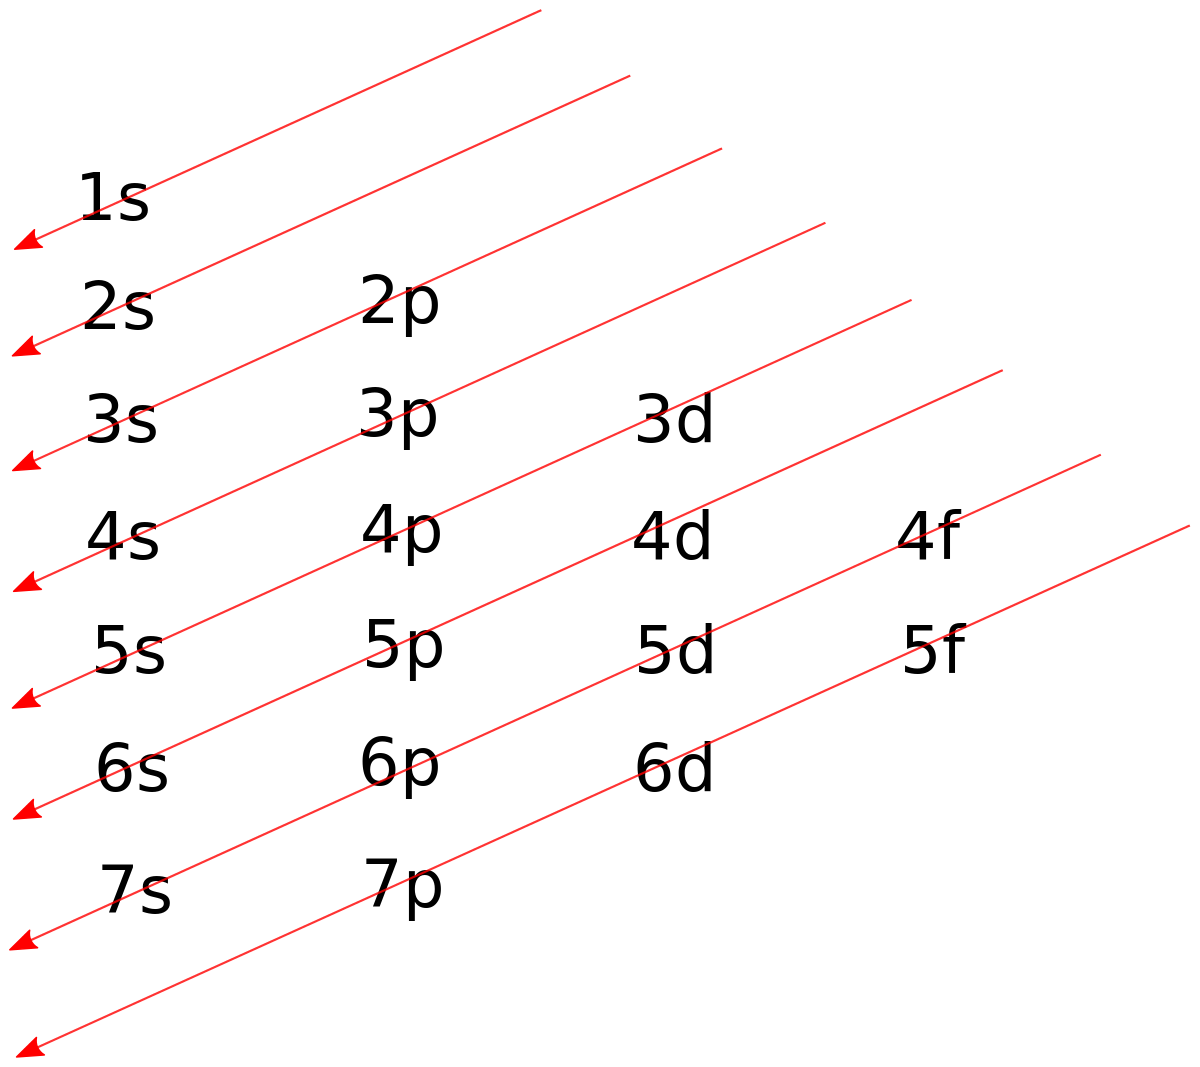
\includegraphics[width=0.3\textwidth]{Aufbau principle}
\end{wrapfigure}
The Aufbau principle states that in the ground state of an atom, electrons fill subshells of the lowest available energy, then they fill subshells of higher energy. The figure on the right summarizes the Aufbau principle.\bigskip\newline
There are exceptions to the Aufbau principle, e.g. the electronic configuration of $\mathbf{Cr}$ and $\mathbf{Cu}$ are $[\mathbf{Ar}]3\text{d}^{5}4\text{s}^{1}$ and $[\mathbf{Ar}]3\text{d}^{10}4\text{s}^{1}$ instead of $[\mathbf{Ar}]3\text{d}^{4}4\text{s}^{2}$ and $[\mathbf{Ar}]3\text{d}^{9}4\text{s}^{2}$ respectively.


\addcontentsline{toc}{section}{Problems}
\section*{Problems}
\begin{problem}
For a hydrogen atom,\bigskip\newline
a) How many electron states are there with principal quantum number $n=3$?\bigskip\newline
b) Among these $n=3$ states, how many states are in the $\text{s}$, $\text{p}$ and $\text{d}$ orbitals respectively?\bigskip\newline
c) Let $E_{3}$ be the energy of this $n=3$ state, now a photon is emitted due to transition involving the $n=3$ state. What is the highest possible frequency of the photon, in terms of $E_{3}$ and the Planck constant $h$?
\end{problem}

\begin{solbox}
a) Put $n=3$,
\begin{align*}
N&=2n^{2}\\
&=18
\end{align*}
b) Number of states in the $\text{s}$, $\text{p}$ and $\text{d}$ orbitals are 2, 6 and 10 respectively.\bigskip\newline
c) For a hydrogen atom, we have $E_{n}=\frac{E_{1}}{n^{2}}$ and $E_{1}<0$. When the electron transits from a higher energy state to a lower energy state, a photon is emitted. The $n=3$ state can be the initial state or the final state.

\subsubsection*{$n=3$ as the initial state}
If $n=3$ is the initial state, it can transit to another state $m=1$, $2$.
\begin{align*}
\D E&=E_{3}-E_{m}\\
h\nu&=\frac{E_{1}}{3^{2}}-\frac{E_{1}}{m^{2}}\\
\nu&=\frac{1}{h}\left(\frac{E_{1}}{9}-\frac{E_{1}}{m^{2}}\right)\\
&\leq\frac{1}{h}\left(\frac{E_{1}}{9}-E_{1}\right)\\
&=-\frac{8E_{3}}{h}
\end{align*}

\subsubsection*{$n=3$ as the final state}
If $n=3$ is the final state, another state $m>3$ can transit to it.
\begin{align*}
\D E&=E_{n}-E_{3}\\
\nu&=\frac{1}{h}\left(\frac{E_{1}}{m^{2}}-\frac{E_{1}}{9}\right)\\
&\leq-\frac{1}{h}\frac{E_{1}}{9}\\
&=-\frac{E_{3}}{h}
\end{align*}
Therefore,
\begin{align*}
\nu_{\text{max}}&=\max\left(-\frac{8E_{3}}{h}, -\frac{E_{3}}{h}\right)\\
&=-\frac{8E_{3}}{h}
\end{align*}
\end{solbox}

\begin{problem}
Find electronic configurations of elements $\mathbf{Be}$, $\mathbf{C}$, $\mathbf{Ne}$ and $\mathbf{K}$.
\end{problem}

\begin{solbox}
Using the Aufbau principle, the electronic configurations are
\begin{align*}
\mathbf{Be}&:1\text{s}^{2}2\text{s}^{2}\\
\mathbf{C}&:1\text{s}^{2}2\text{s}^{2}2\text{p}^{2}\\
\mathbf{Ne}&:1\text{s}^{2}2\text{s}^{2}2\text{p}^{6}\\
\mathbf{K}&:1\text{s}^{2}2\text{s}^{2}2\text{p}^{6}3\text{s}^{2}3\text{p}^{6}4\text{s}^{1}
\end{align*}
\end{solbox}

\subsection*{2019-20 Fall Final Q2 - The hydrogen atom}
\label{The hydrogen atom}
Given the vacuum permittivity $\e_{0}$, electron mass $m$, electron charge $e$, Planck constant $h$ and speed of light $c$, derive the energy of the ground state for a hydrogen atom. You can use either Bohr's original proposal or de Broglie's matter wave approach.

\begin{solbox}
Bohr's method is given in the notes, so we will use de Broglie's matter wave approach.\bigskip\newline
The centripetal force on the electron is provided by the Coulomb force,
\begin{align*}
\frac{mv^{2}}{r}&=\frac{1}{4\pi\e_{0}}\frac{e^{2}}{r^{2}}\\
\implies mv^{2}r&=\frac{e^{2}}{4\pi\e_{0}}
\end{align*}
The potential energy of the electron is given by $V(r)=-\frac{1}{4\pi\e_{0}}\frac{e^{2}}{r}$, so its total energy is
\begin{align*}
E&=\frac{1}{2}mv^{2}+V(r)\\
&=-\frac{1}{2}mv^{2}\\
&=-\frac{1}{2}\cdot\frac{e^{2}}{4\pi\e_{0}r}
\end{align*}
According to de Broglie's approach, an integral multiple of wavelength must fit within the circumference of the orbit,
\begin{align*}
2\pi r=n\l
\end{align*}
and the wavelength of the matter wave is given by
\begin{align*}
\l=\frac{h}{mv}
\end{align*}
Combining these two equations,
\begin{align*}
mvr=\frac{nh}{2\pi}
\end{align*}
The speed $v$ of the electron is thus
\begin{align*}
v=\frac{mv^{2}r}{mvr}&=\frac{e^{2}}{4\pi\e_{0}}\cdot \frac{2\pi}{nh}\\
&=\frac{e^{2}}{2\e_{0}nh}
\end{align*}
Substitute the result to the total energy,
\begin{align*}
E_{n}&=-\frac{1}{2}mv^{2}\\
&=-\frac{1}{2}m\cdot \frac{e^{4}}{4\e_{0}^{2}n^{2}h^{2}}\\
&=-\frac{me^{4}}{8\e_{0}^{2}n^{2}h^{2}}
\end{align*}
The ground state corresponds to $n=1$, so the energy is
\begin{align*}
E_{1}=-\frac{me^{4}}{8\e_{0}^{2}n^{2}h^{2}}
\end{align*}
\end{solbox}

\subsection*{2020-21 Fall Final Q3 - Transition of the Helium ion}
For the Helium ion $\mathbf{He}^{+}$ (Helium nuclei with one electron), use the Bohr's model (either his original model, or complemented with de Broglie's quantization) to calculate the frequency of light emitted from a transition between $n_{1}$ and $n_{2}$ states.

\begin{solbox}
The solution is very similar to the above one, but this time we consider a hydrogen-like atom with nuclear charge $Z$.\bigskip\newline
The centripetal force on the electron is provided by the Coulomb force,
\begin{align*}
\frac{mv^{2}}{r}&=\frac{1}{4\pi\e_{0}}\frac{Ze^{2}}{r^{2}}\\
\implies mv^{2}r&=\frac{Ze^{2}}{4\pi\e_{0}}
\end{align*}
The potential energy of the electron is given by $V(r)=-\frac{1}{4\pi\e_{0}}\frac{Ze^{2}}{r}$, so its total energy is
\begin{align*}
E&=\frac{1}{2}mv^{2}+V(r)\\
&=-\frac{1}{2}mv^{2}\\
&=-\frac{1}{2}\cdot\frac{Ze^{2}}{4\pi\e_{0}r}
\end{align*}
Using de Broglie's approach,
\begin{align*}
2\pi r&=n\l\\
\l&=\frac{h}{mv}
\end{align*}
Combining these two equations,
\begin{align*}
mvr=\frac{nh}{2\pi}
\end{align*}
The speed $v$ of the electron is thus
\begin{align*}
v=\frac{mv^{2}r}{mvr}&=\frac{Ze^{2}}{4\pi\e_{0}}\cdot \frac{2\pi}{nh}\\
&=\frac{Ze^{2}}{2\e_{0}nh}
\end{align*}
Substitute the result to the total energy,
\begin{align*}
E_{n}&=-\frac{1}{2}mv^{2}\\
&=-\frac{1}{2}m\cdot \frac{Z^{2}e^{4}}{4\e_{0}^{2}n^{2}h^{2}}\\
&=-\frac{Z^{2}me^{4}}{8\e_{0}^{2}n^{2}h^{2}}
\end{align*}
When the electron transits from the $n_{1}$ state to the $n_{2}$ state, the difference in energy is
\begin{align*}
\D E=-\frac{Z^{2}me^{4}}{8\e_{0}^{2}h^{2}}\left(\frac{1}{n_{1}^{2}}-\frac{1}{n_{2}^{2}}\right)
\end{align*}
The Helium ion has $Z=2$, so the frequency of light emitted is
\begin{align*}
\nu&=-\frac{Z^{2}me^{4}}{8\e_{0}^{2}h^{3}}\left(\frac{1}{n_{1}^{2}}-\frac{1}{n_{2}^{2}}\right)\\
&=-\frac{me^{4}}{2\e_{0}^{2}h^{3}}\left(\frac{1}{n_{1}^{2}}-\frac{1}{n_{2}^{2}}\right)
\end{align*}
\end{solbox}

\newpage
\chapterimage{Chapter 6} % Chapter heading image
\chapter{Quantum entanglement}
\section{Stern-Gerlach experiment}
In the experiment, a beam of hot silver atoms passes through an inhomogeneous magnetic field, and the outgoing silver atoms leave records on a screen. It is observed that one beam splits into two beams with equal strength. Such observation has the following quantum interpretation.
\begin{itembox}
\begin{itemize}
\item The magnitude $|\vec{\mu}|$ of the silver atom is quantized.
\item Since the external magnetic field measures $\mu_{z}$ of the atoms, the state of each atom collapses to one of the two eigenstates with eigenvalue $\pm|\vec{\mu}|$. 
\item The two eigenstates of the spin in the $z$-direction are $\ket{\uparrow}$ with eigenvalue $|\vec{\mu}|$ and $\ket{\downarrow}$ with eigenvalue $-|\vec{\mu}|$ respectively.
\end{itemize}
\end{itembox}
The magnetic moment of the silver atom comes from the magnetic moment of its outermost $5\text{s}$ electron, showing that the electron has magnetic moment. The intrinsic magnetic moment of an electron is called ``spin".\bigskip\newline
However, the term ``spin" is more general than magnetic moment for fundamental particles. A particle with non-zero spin does not always have non-zero magnetic moment, e.g. a photon has spin $1$ but zero magnetic moment.

\section{Spins}
The superpositions of $\ket{\uparrow}$ and $\ket{\downarrow}$ form other orientations, including $\ket{\rightarrow}$, $\ket{\leftarrow}$, $\ket{\otimes}$ and $\ket{\odot}$. It is convenient to choose the following conventions.
\begin{eqnbox}
\begin{align}
\ket{\rightarrow}&=\frac{1}{\sqrt{2}}\left(\ket{\uparrow}+\ket{\downarrow}\right), &\ket{\leftarrow}=\frac{1}{\sqrt{2}}\left(\ket{\uparrow}-\ket{\downarrow}\right)\nonumber\\
\ket{\otimes}&=\frac{1}{\sqrt{2}}\left(\ket{\uparrow}+i\ket{\downarrow}\right), &\ket{\odot}=\frac{1}{\sqrt{2}}\left(\ket{\uparrow}-i\ket{\downarrow}\right)
\end{align}
\end{eqnbox}

\begin{wrapfigure}[5]{r}{0.4\textwidth}
\centering
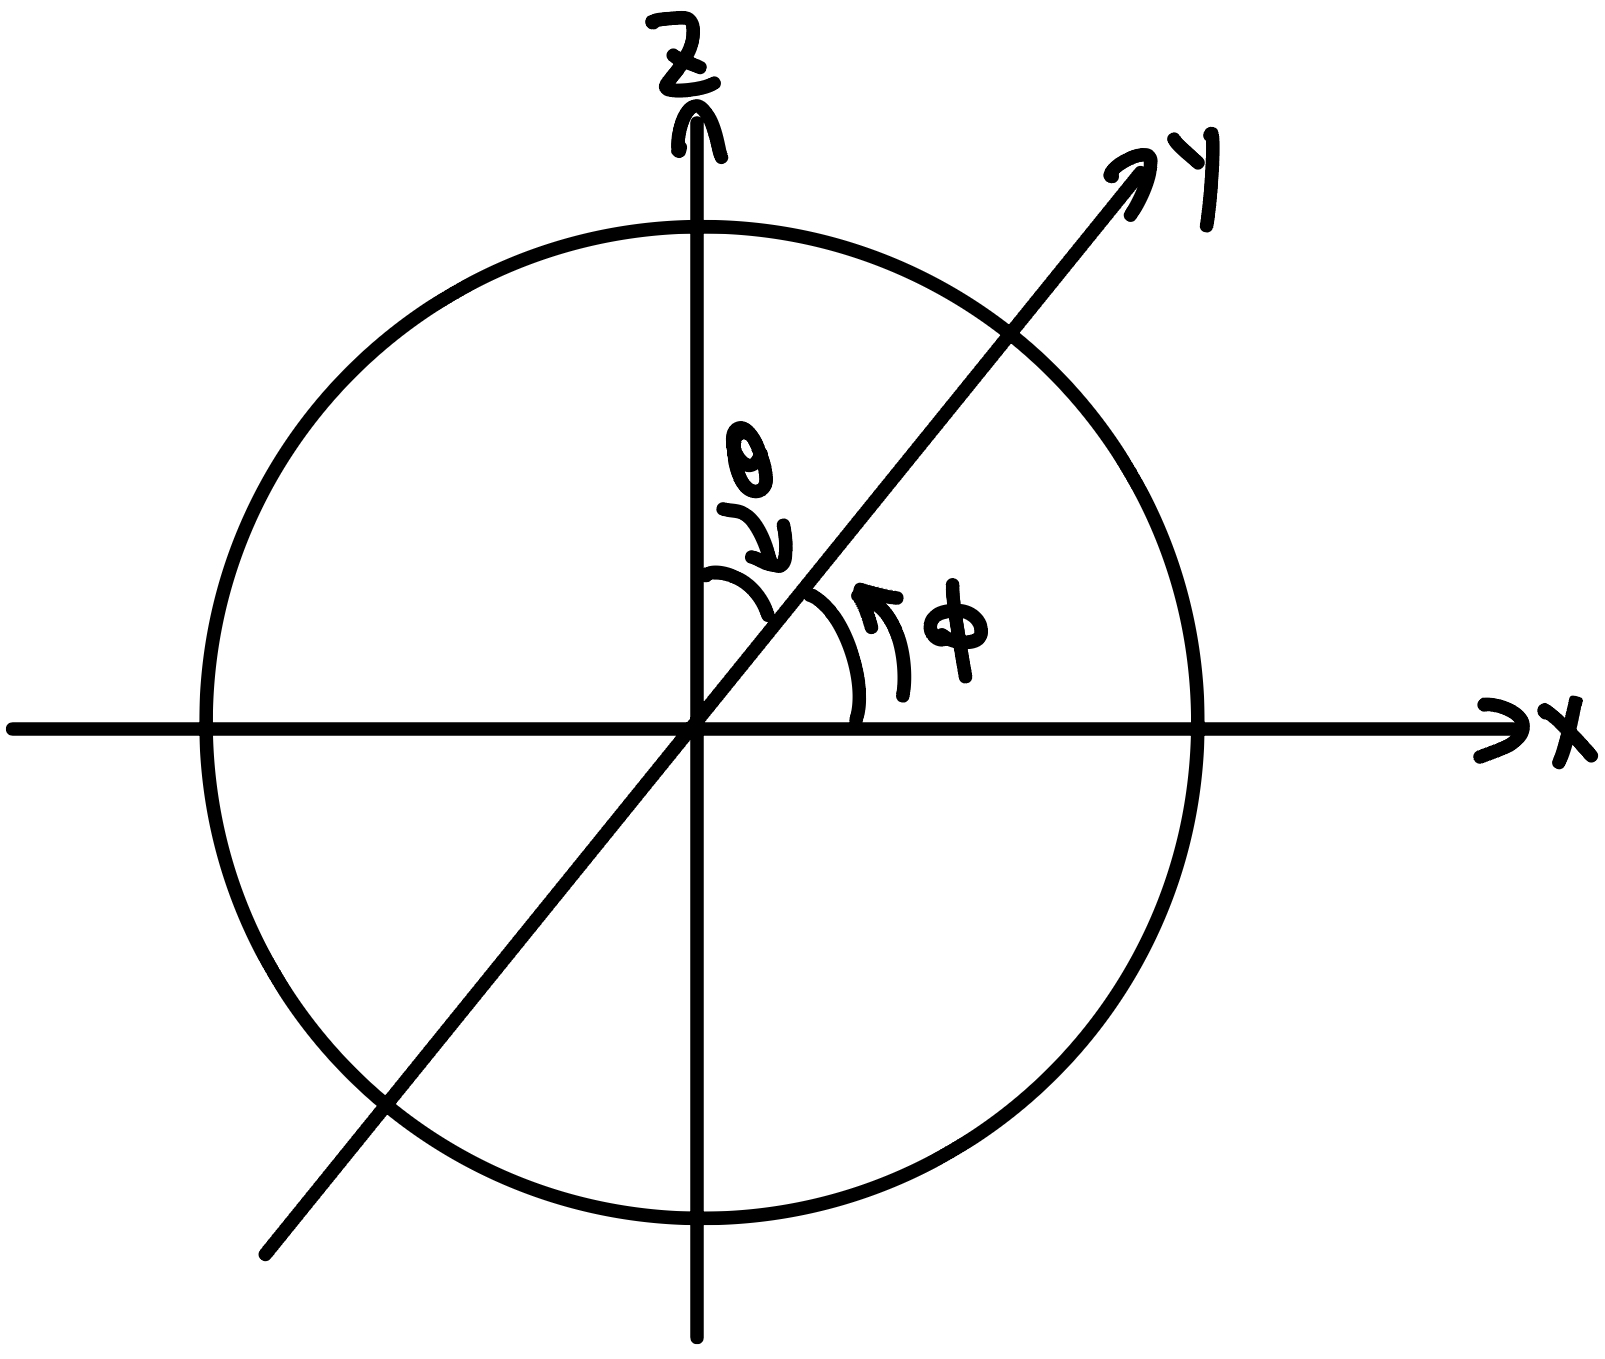
\includegraphics[width=0.3\textwidth]{Bloch sphere}
\end{wrapfigure}

\noindent A spin state can be thought as a qubit of information, and a general state is
\begin{eqnbox}
\begin{align}
\ket{\psi}=\cos\left(\frac{\theta}{2}\right)\ket{\uparrow}+e^{i\phi}\sin\left(\frac{\theta}{2}\right)\ket{\downarrow}
\end{align}
\end{eqnbox}

\noindent where $0\leq\theta\leq\pi$ and $0\leq\phi<2\pi$. The Bloch sphere illustrated on the right is a geometric representation of a qubit.\bigskip\newline
We can express the superpositions of spin states using eq. (6.2), e.g. in the $x$-direction,
\begin{align*}
\ket{\rightarrow}&: \theta=\frac{\pi}{2}, \phi=0\\
\ket{\leftarrow}&: \theta=\frac{\pi}{2}, \phi=\pi
\end{align*}
and in the $y$-direction,
\begin{align*}
\ket{\otimes}&: \theta=\frac{\pi}{2}, \phi=\frac{\pi}{2}\\
\ket{\odot}&: \theta=\frac{\pi}{2}, \phi=\frac{3\pi}{2}
\end{align*}
Try to visualize these spin states using the Bloch sphere in your mind.\bigskip\newline
Choosing $\ket{\uparrow}$ and $\ket{\downarrow}$ as the basis, the states in the $z$, $x$ and $y$-direction are
\begin{eqnbox}
\begin{align}
\ket{\uparrow}&=
\begin{pmatrix}
1\\
0
\end{pmatrix}, &
\ket{\downarrow}&=
\begin{pmatrix}
0\\
1
\end{pmatrix},\nonumber\\
\ket{\rightarrow}&=\frac{1}{\sqrt{2}}
\begin{pmatrix}
1\\
1
\end{pmatrix}, &
\ket{\leftarrow}&=\frac{1}{\sqrt{2}}
\begin{pmatrix}
1\\
-1
\end{pmatrix},\nonumber\\
\ket{\otimes}&=\frac{1}{\sqrt{2}}
\begin{pmatrix}
1\\
i
\end{pmatrix}, &
\ket{\odot}&=\frac{1}{\sqrt{2}}
\begin{pmatrix}
1\\
-i
\end{pmatrix}
\end{align}
\end{eqnbox}

\subsection*{Normalization and orthogonality of spin states}
The normalization conditions of spin states are
\begin{eqnbox}
\begin{align}
\braket{\uparrow}=\braket{\downarrow}=\braket{\rightarrow}=\braket{\leftarrow}=\braket{\otimes}=\braket{\odot}=1
\end{align}
\end{eqnbox}

\noindent and the corresponding pair of states are orthogonal to each other,
\begin{eqnbox}
\begin{align}
\braket{\uparrow}{\downarrow}=\braket{\rightarrow}{\leftarrow}=\braket{\otimes}{\odot}=0
\end{align}
\end{eqnbox}

\subsection*{Operators for spin measurements}
For spin-$\frac{1}{2}$ particles, the spin operators are Pauli matrices, which measure the spin of a state and give eigenvalues $\pm1$. The operators are
\begin{eqnbox}
\begin{align}
\s_{3}=
\begin{pmatrix}
1&0\\
0&-1
\end{pmatrix}, &&
\s_{1}=
\begin{pmatrix}
0&1\\
1&0
\end{pmatrix}, &&
\s_{2}=
\begin{pmatrix}
0&-i\\
i&0
\end{pmatrix}
\end{align}
\end{eqnbox}
which correspond to measurements of spin in the $z$, $x$ and $y$-direction respectively.
\begin{example}[Spin in the $x$-direction]
Let's consider the measurements of spin in the $x$-direction. We should use the $\s_{1}$ operator.
\begin{align*}
\s_{1}\ket{\rightarrow}&=
\begin{pmatrix}
0&1\\
1&0
\end{pmatrix}
\frac{1}{\sqrt{2}}
\begin{pmatrix}
1\\
1
\end{pmatrix}\\
&=\frac{1}{\sqrt{2}}
\begin{pmatrix}
1\\
1
\end{pmatrix}\\
&=\ket{\rightarrow}\\
\s_{1}\ket{\leftarrow}&=
\begin{pmatrix}
0&1\\
1&0
\end{pmatrix}
\frac{1}{\sqrt{2}}
\begin{pmatrix}
1\\
-1
\end{pmatrix}\\
&=\frac{1}{\sqrt{2}}
\begin{pmatrix}
-1\\
1
\end{pmatrix}\\
&=-\ket{\leftarrow}
\end{align*}
$\s_{1}$ measures spin states in the $x$-direction and gives eigenvalues $\pm1$. The measurements of spin using $\s_{2}$ and $\s_{3}$ are similar (see \hyperref[Problem 6.1]{Problem 6.1}).
\end{example}
\noindent
By direct matrix calculation, it is interesting to notice that
\begin{eqnbox}
\begin{align}
\s_{1}\ket{\uparrow}=\ket{\downarrow}, &&\s_{1}\ket{\downarrow}=\ket{\uparrow}, &&\s_{2}\ket{\uparrow}=i\ket{\downarrow}, &&\s_{2}\ket{\downarrow}=-i\ket{\uparrow}
\end{align}
\end{eqnbox}
The operator for measurement in a general direction $\hat{n}$ is
\begin{eqnbox}
\begin{align}
\s(\hat{n})\equiv\sum_{i}\hat{n}_{i}\s_{i}=\hat{n}\cdot\vec{\s}
\end{align}
\end{eqnbox}
where the Pauli matrices are combined into the ``Pauli vector",
\begin{align*}
\vec{\s}\equiv\s_{1}\hat{i}+\s_{2}\hat{j}+\s_{3}\hat{k}
\end{align*}
\begin{example}
Along $45^\circ$ direction of the $x$-$z$ plane, $\hat{n}=\frac{1}{\sqrt{2}}\left(\hat{i}+\hat{k}\right)$. This means
\begin{align*}
\s(\hat{n})=\hat{n}\cdot\vec{\s}=\frac{1}{\sqrt{2}}\left(\s_{1}+\s_{3}\right)
\end{align*}
\end{example}

\subsection*{Probabilities of spin measurements}
For a spin state $\ket{\psi}$, when measuring the spin of the $z$-direction, the probability to find the spin up state is
\begin{eqnbox}
\begin{align}
P_{\uparrow}=\bra{\psi}\frac{1+\s_{3}}{2}\ket{\psi}
\end{align}
\end{eqnbox}
It is because the spin state $\ket{\psi}$ can be decomposed into
\begin{align*}
\ket{\psi}=\a_{1}\ket{\uparrow}+\a_{2}\ket{\downarrow}
\end{align*}
Note that $\frac{1+\s_{3}}{2}\ket{\uparrow}=\ket{\uparrow}$ and $\frac{1+\s_{3}}{2}\ket{\downarrow}=0$, hence
\begin{align*}
\bra{\psi}\frac{1+\s_{3}}{2}\ket{\psi}={\left|\a_{1}\right|}^{2}=P_{\uparrow}
\end{align*}
The probability to find a spin state $\ket{\psi}$ along the $\hat{n}$ direction after a corresponding measurement is
\begin{eqnbox}
\begin{align}
P_{\hat{n}}=\bra{\psi}\frac{1+\s(\hat{n})}{2}\ket{\psi}
\end{align}
\end{eqnbox}

\section{Multiple spins and entanglement}
When we have two spins, a general state is
\begin{eqnbox}
\begin{align}
\ket{\psi}=\a_{1}\ket{\uparrow\uparrow}+\a_{2}\ket{\uparrow\downarrow}+\a_{3}\ket{\downarrow\uparrow}+\a_{4}\ket{\downarrow\downarrow}
\end{align}
\end{eqnbox}
The state contains two qubits of information.\bigskip\newline
Each spin state is described by $2\times2-2=2$ real parameters (two complex parameters deducting normalization and an overall phase), so we may expect two non-interacting spins are described by $2\times2=4$ real parameters. But in eq. (6.11), there are four complex parameters, thus after deducting normalization and an overall phase, two non-interacting spins together need $4\times2-2=6$ real parameters to describe. The extra two parameters describe the entanglement of the two states.\bigskip\newline
More generally, a state with $n$ qubits is described by $2^{n+1}-2$ real parameters.\bigskip\newline
For simplicity, we only consider measurements that operates separately on each individual qubit. Let $\s_{i}$ be the Pauli matrices on particle $1$, and $\t_{i}$ be the Pauli matrices on particle $2$. For example, with the aid of eq. (6.7),
\begin{align*}
\s_{1}\ket{\uparrow\downarrow}=\ket{\downarrow\downarrow}, \,\,\,\,\,\t_{1}\ket{\uparrow\downarrow}=\ket{\uparrow\uparrow}
\end{align*}
Since $\s_{1}$ and $\t_{1}$ act on different spin states, the order of operations $\s_{i}$ and $\t_{i}$ commute, e.g. $\s_{1}\t_{1}\ket{\uparrow\downarrow}=\t_{1}\s_{1}\ket{\uparrow\downarrow}=\ket{\downarrow\uparrow}$.\bigskip\newline
The probability to find particle $1$ in the direction $\hat{n}$ and particle $2$ in the direction $\hat{m}$ is then
\begin{eqnbox}
\begin{align}
P_{\hat{n}\hat{m}}=\bra{\psi}\frac{1+\s(\hat{n})}{2}\frac{1+\t(\hat{m})}{2}\ket{\psi}
\end{align}
\end{eqnbox}

\section{EPR paradox}
Consider the singlet state
\begin{eqnbox}
\begin{align}
\ket{s}=\frac{1}{\sqrt{2}}\left(\ket{\uparrow\downarrow}-\ket{\downarrow\uparrow}\right)
\end{align}
\end{eqnbox}
and take the two particles far apart each other. Alice receives particle $1$ and Bob receives particle $2$. They then measure the spin of the particles along the $z$-direction immediately after receiving the particles. Using eq. (6.12),
\begin{align*}
P_{\uparrow\uparrow}&=\bra{s}\frac{1+\s_{3}}{2}\frac{1+\t_{3}}{2}\ket{s}\\
\frac{1+\s_{3}}{2}\frac{1+\t_{3}}{2}\ket{s}&=\frac{1}{4\sqrt{2}}(1+\s_{3}+\t_{3}+\s_{3}\t_{3})\left(\ket{\uparrow\downarrow}-\ket{\downarrow\uparrow}\right)\\
&=\frac{1}{4\sqrt{2}}\left(\ket{\uparrow\downarrow}-\ket{\downarrow\uparrow}+\ket{\uparrow\downarrow}+\ket{\downarrow\uparrow}-\ket{\uparrow\downarrow}-\ket{\downarrow\uparrow}-\ket{\uparrow\downarrow}+\ket{\downarrow\uparrow}\right)\\
&=0\\
\implies P_{\uparrow\uparrow}&=0\\
P_{\uparrow\downarrow}&=\bra{s}\frac{1+\s_{3}}{2}\frac{1-\t_{3}}{2}\ket{s}\\
\frac{1+\s_{3}}{2}\frac{1-\t_{3}}{2}\ket{s}&=\frac{1}{4\sqrt{2}}(1+\s_{3}-\t_{3}-\s_{3}\t_{3})\left(\ket{\uparrow\downarrow}-\ket{\downarrow\uparrow}\right)\\
&=\frac{1}{4\sqrt{2}}\left(\ket{\uparrow\downarrow}-\ket{\downarrow\uparrow}+\ket{\uparrow\downarrow}+\ket{\downarrow\uparrow}+\ket{\uparrow\downarrow}+\ket{\downarrow\uparrow}+\ket{\uparrow\downarrow}-\ket{\downarrow\uparrow}\right)\\
&=\frac{1}{\sqrt{2}}\ket{\uparrow\downarrow}\\
\implies P_{\uparrow\downarrow}&=\bra{s}\frac{1}{\sqrt{2}}\ket{\uparrow\downarrow}\\
&=\frac{1}{\sqrt{2}}\left(\bra{\uparrow\downarrow}-\bra{\downarrow\uparrow}\right)\frac{1}{\sqrt{2}}\ket{\uparrow\downarrow}\\
&=\frac{1}{2}
\end{align*}
Similarly, we find that $P_{\downarrow\uparrow}=\frac{1}{2}$ and $P_{\downarrow\downarrow}=0$. Alice and Bob have equal chance to find the state having spin up or down. In other words, when we measure each of the particle in the EPR pair individually, random result is obtained.\bigskip\newline
The results of Alice and Bob are totally correlated -- if one gets up, the other must get down. As long as they are measuring along the same direction $\hat{n}$, the correlation exists. This is the physical indication of entanglement.

\section{Local hidden variable theory}
Is it possible that the random outcome of EPR is determined when the two spin states are together, and each state follows classical logic after separation? This implies a local hidden theory that needs to satisfy the followings,
\begin{itembox}
\begin{itemize}
\item Hidden variable: the apparent quantum behaviour follows some classical logic.
\item Local: space-like measurements do not affect each other.
\end{itemize}
\end{itembox}
One consequence of classical logic is
\begin{eqnbox}
\begin{align}
P(A, \neg B)+P(B, \neg C)\geq P(A, \neg C)
\end{align}
\end{eqnbox}
which can be demonstrated with a Venn diagram. Now, we test whether the singlet state is consistent with eq. (6.14). We define $A$, $B$ and $C$ as measurements by Alice,\bigskip\newline
$A$: Measure particle $1$ along the $z$-axis and get positive spin.\bigskip\newline
$B$: Measure particle $1$ along the $45^\circ$ in $x$-$z$ plane and get positive spin.\bigskip\newline
$C$: Measure particle $1$ along the $x$-axis and get positive spin.\bigskip\newline
The negations of $A$, $B$ and $C$ are related to measurements by Bob,\bigskip\newline
$\neg A$: Measure particle $2$ along the $z$-axis and get positive spin.\bigskip\newline
$\neg B$: Measure particle $2$ along the $45^\circ$ in $x$-$z$ plane and get positive spin.\bigskip\newline
$\neg C$: Measure particle $2$ along the $x$-axis and get positive spin.\bigskip\newline
eq. (6.14) with the above conditions is known as the Bell's inequality.  The probabilities of the events are
\begin{eqnbox}
\begin{align}
P(A, \neg B)&=\bra{s}\frac{1+\s_{3}}{2}\frac{1+\frac{1}{\sqrt{2}}\left(\t_{1}+\t_{3}\right)}{2}\ket{s}=\frac{1}{4}\left(1-\frac{1}{\sqrt{2}}\right)\nonumber\\
P(B, \neg C)&=\bra{s}\frac{1+\frac{1}{\sqrt{2}}\left(\s_{1}+\s_{3}\right)}{2}\frac{1+\t_{1}}{2}\ket{s}=\frac{1}{4}\left(1-\frac{1}{\sqrt{2}}\right)\nonumber\\
P(A, \neg C)&=\bra{s}\frac{1+\s_{3}}{2}\frac{1+\t_{1}}{2}\ket{s}=\frac{1}{4}
\end{align}
\end{eqnbox}
The classical logic eq. (6.14) is violated by the EPR paradox. Therefore, the nature of EPR pairs cannot be mimicked by a local hidden variable theory.

\addcontentsline{toc}{section}{Problems}
\section*{Problems}
\begin{problem}
\label{Problem 6.1}
Verify that $\s_{2}$ and $\s_{3}$ measure spin states in the $y$ and $z$-directions respectively, and give eigenvalues $\pm1$.
\end{problem}

\begin{solbox}
In the $y$-direction,
\begin{align*}
\s_{2}\ket{\otimes}&=
\begin{pmatrix}
0&-i\\
i&0
\end{pmatrix}
\frac{1}{\sqrt{2}}
\begin{pmatrix}
1\\
i
\end{pmatrix}\\
&=\frac{1}{\sqrt{2}}
\begin{pmatrix}
1\\
i
\end{pmatrix}\\
&=\ket{\otimes}\\
\s_{2}\ket{\odot}&=
\begin{pmatrix}
0&-i\\
i&0
\end{pmatrix}
\frac{1}{\sqrt{2}}
\begin{pmatrix}
1\\
-i
\end{pmatrix}\\
&=\frac{1}{\sqrt{2}}
\begin{pmatrix}
-1\\
i
\end{pmatrix}\\
&=-\ket{\odot}
\end{align*}
In the $z$-direction,
\begin{align*}
\s_{3}\ket{\uparrow}&=
\begin{pmatrix}
1&0\\
0&-1
\end{pmatrix}
\begin{pmatrix}
1\\
0
\end{pmatrix}\\
&=
\begin{pmatrix}
1\\
0
\end{pmatrix}\\
&=\ket{\uparrow}\\
\s_{3}\ket{\downarrow}&=
\begin{pmatrix}
1&0\\
0&-1
\end{pmatrix}
\begin{pmatrix}
0\\
1
\end{pmatrix}\\
&=
\begin{pmatrix}
0\\
-1
\end{pmatrix}\\
&=-\ket{\downarrow}
\end{align*}
\end{solbox}

\begin{problem}
Compute the probabilities $P(A, \neg B)$, $P(B, \neg C)$ and $P(A, \neg C)$ shown in eq. (6.15).
\end{problem}

\begin{solbox}
\begin{align*}
P(A, \neg B)&=\bra{s}\frac{1+\s_{3}}{2}\frac{1+\frac{1}{\sqrt{2}}\left(\t_{1}+\t_{3}\right)}{2}\ket{s}\\
\frac{1+\s_{3}}{2}\frac{1+\frac{1}{\sqrt{2}}\left(\t_{1}+\t_{3}\right)}{2}\ket{s}&=\frac{1}{4\sqrt{2}}\left(1+\s_{3}\right)\left(1+\frac{1}{\sqrt{2}}\left(\t_{1}+\t_{3}\right)\right)\left(\ket{\uparrow\downarrow}-\ket{\downarrow\uparrow}\right)\\
&=\frac{1}{4\sqrt{2}}\left(1+\frac{\t_{1}}{\sqrt{2}}+\frac{\t_{3}}{\sqrt{2}}+\s_{3}+\frac{\s_{3}\t_{1}}{\sqrt{2}}+\frac{\s_{3}\t_{3}}{\sqrt{2}}\right)\left(\ket{\uparrow\downarrow}-\ket{\downarrow\uparrow}\right)\\
\end{align*}
By direct computation,
\begin{align*}
&\t_{1}\ket{\uparrow\downarrow}=\ket{\uparrow\uparrow}, \t_{1}\ket{\downarrow\uparrow}=\ket{\downarrow\downarrow}, \t_{3}\ket{\uparrow\downarrow}=-\ket{\uparrow\downarrow}, \t_{3}\ket{\downarrow\uparrow}=\ket{\downarrow\uparrow}, \s_{3}\ket{\uparrow\downarrow}=\ket{\uparrow\downarrow}, \s_{3}\ket{\downarrow\uparrow}=-\ket{\downarrow\uparrow}\\
&\t_{1}\s_{3}\ket{\uparrow\downarrow}=\ket{\uparrow\uparrow}, \t_{1}\s_{3}\ket{\downarrow\uparrow}=-\ket{\downarrow\downarrow}, \t_{3}\s_{3}\ket{\uparrow\downarrow}=-\ket{\uparrow\downarrow}, \t_{3}\s_{3}\ket{\downarrow\uparrow}=-\ket{\downarrow\uparrow}
\end{align*}
After substitution,
\begin{align*}
\frac{1+\s_{3}}{2}\frac{1+\frac{1}{\sqrt{2}}\left(\t_{1}+\t_{3}\right)}{2}\ket{s}&=\frac{1}{4\sqrt{2}}\bigg(\ket{\uparrow\downarrow}-\ket{\downarrow\uparrow}+\frac{1}{\sqrt{2}}\ket{\uparrow\uparrow}-\frac{1}{\sqrt{2}}\ket{\downarrow\downarrow}-\frac{1}{\sqrt{2}}\ket{\uparrow\downarrow}-\frac{1}{\sqrt{2}}\ket{\downarrow\uparrow}\\
&\,\,\,\,\,\,\,+\ket{\uparrow\downarrow}+\ket{\downarrow\uparrow}+\frac{1}{\sqrt{2}}\ket{\uparrow\uparrow}+\frac{1}{\sqrt{2}}\ket{\downarrow\downarrow}-\frac{1}{\sqrt{2}}\ket{\uparrow\downarrow}+\frac{1}{\sqrt{2}}\ket{\downarrow\uparrow}\bigg)\\
&=\frac{1}{4\sqrt{2}}\left(\left(2-\sqrt{2}\right)\ket{\uparrow\downarrow}+\sqrt{2}\ket{\uparrow\uparrow}\right)\\
\implies P(A, \neg B)&=\bra{s}\frac{1}{4\sqrt{2}}\left(\left(2-\sqrt{2}\right)\ket{\uparrow\downarrow}+\sqrt{2}\ket{\uparrow\uparrow}\right)\\
&=\frac{1}{\sqrt{2}}\left(\bra{\uparrow\downarrow}-\bra{\downarrow\uparrow}\right)\frac{1}{4\sqrt{2}}\left(\left(2-\sqrt{2}\right)\ket{\uparrow\downarrow}+\sqrt{2}\ket{\uparrow\uparrow}\right)\\
&=\frac{1}{4}\left(1-\frac{1}{\sqrt{2}}\right)
\end{align*}
It is unnecessary to compute $P(B, \neg C)$ directly. The probabilities of the events remain the same if we swap Alice $\leftrightarrow$ Bob and particle $1\leftrightarrow2$, so $P(B, \neg C)=P(\neg B, C)$. By symmetry, we can also swap the $x$ and $z$-axes, which implies $P(\neg B, C)=P(A, \neg B)$. Combining both arguments, we know $P(B, \neg C)=P(A, \neg B)=\frac{1}{4}\left(1-\frac{1}{\sqrt{2}}\right)$.
\begin{align*}
P(A, \neg C)&=\bra{s}\frac{1+\s_{3}}{2}\frac{1+\t_{1}}{2}\ket{s}\\
\frac{1+\s_{3}}{2}\frac{1+\t_{1}}{2}\ket{s}&=\frac{1}{4\sqrt{2}}\left(1+\s_{3}+\t_{1}+\s_{3}\t_{1}\right)\left(\ket{\uparrow\downarrow}-\ket{\downarrow\uparrow}\right)\\
&=\frac{1}{4\sqrt{2}}\left(\ket{\uparrow\downarrow}-\ket{\downarrow\uparrow}+\ket{\uparrow\downarrow}+\ket{\downarrow\uparrow}+\ket{\uparrow\downarrow}-\ket{\downarrow\uparrow}+\ket{\uparrow\downarrow}+\ket{\downarrow\uparrow}\right)\\
&=\frac{1}{4\sqrt{2}}\left(2\ket{\uparrow\downarrow}+2\ket{\uparrow\uparrow}\right)\\
\implies P(A, \neg C)&=\bra{s}\frac{1}{4\sqrt{2}}\left(2\ket{\uparrow\downarrow}+2\ket{\uparrow\uparrow}\right)\\
&=\frac{1}{\sqrt{2}}\left(\bra{\uparrow\downarrow}-\bra{\downarrow\uparrow}\right)\frac{1}{4\sqrt{2}}\left(2\ket{\uparrow\downarrow}+2\ket{\uparrow\uparrow}\right)\\
&=\frac{1}{4}
\end{align*}
\end{solbox}

\begin{problem}
Consider a state $\ket{\psi}=\a\left(\ket{\uparrow\downarrow}+\ket{\downarrow\uparrow}\right)$.\bigskip\newline
a) Find the normalization constant $\a$.\bigskip\newline
b) When measuring spins in the $z$-direction, what is the probability of getting $\ket{\uparrow\uparrow}$?\bigskip\newline
c) When measuring spins in the $x$-direction, what is the probability of getting $\ket{\rightarrow\rightarrow}$?
\end{problem}

\begin{solbox}
a) $\ket{\psi}$ satisfies the normalization condition $\braket{\psi}=1$.
\begin{align*}
\a\left(\bra{\uparrow\downarrow}+\bra{\downarrow\uparrow}\right)\a\left(\ket{\uparrow\downarrow}+\ket{\uparrow\downarrow}\right)&=1\\
\a^{2}\left(\braket{\uparrow\downarrow}+\braket{\uparrow\downarrow}{\downarrow\uparrow}+\braket{\downarrow\uparrow}{\uparrow\downarrow}+\braket{\downarrow\uparrow}\right)&=1\\
2\a^{2}&=1\\
\a&=\frac{1}{\sqrt{2}}
\end{align*}
b)
\begin{align*}
P_{\uparrow\uparrow}&=\bra{\psi}\frac{1+\s_{3}}{2}\frac{1+\t_{3}}{2}\ket{\psi}\\
\frac{1+\s_{3}}{2}\frac{1+\t_{3}}{2}\ket{\psi}&=\frac{1}{4\sqrt{2}}\left(1+\s_{3}+\t_{3}+\s_{3}\t_{3}\right)\left(\ket{\uparrow\downarrow}+\ket{\downarrow\uparrow}\right)\\
&=\frac{1}{4\sqrt{2}}\left(\ket{\uparrow\downarrow}+\ket{\downarrow\uparrow}+\ket{\uparrow\downarrow}-\ket{\downarrow\uparrow}-\ket{\uparrow\downarrow}+\ket{\downarrow\uparrow}-\ket{\uparrow\downarrow}-\ket{\downarrow\uparrow}\right)\\
&=0\\
\implies P_{\uparrow\uparrow}&=0
\end{align*}
c)
\begin{align*}
P_{\rightarrow\rightarrow}&=\bra{\psi}\frac{1+\s_{1}}{2}\frac{1+\t_{1}}{2}\ket{\psi}\\
\frac{1+\s_{1}}{2}\frac{1+\t_{1}}{2}\ket{\psi}&=\frac{1}{4\sqrt{2}}\left(1+\s_{1}+\t_{1}+\s_{1}\t_{1}\right)\left(\ket{\uparrow\downarrow}+\ket{\downarrow\uparrow}\right)\\
&=\frac{1}{4\sqrt{2}}\left(\ket{\uparrow\downarrow}+\ket{\downarrow\uparrow}+\ket{\downarrow\downarrow}+\ket{\uparrow\uparrow}+\ket{\uparrow\uparrow}+\ket{\downarrow\downarrow}+\ket{\downarrow\uparrow}+\ket{\uparrow\downarrow}\right)\\
&=\frac{1}{4\sqrt{2}}\left(2\ket{\uparrow\downarrow}+2\ket{\downarrow\uparrow}+2\ket{\uparrow\uparrow}+2\ket{\downarrow\downarrow}\right)\\
\implies P_{\rightarrow\rightarrow}&=\bra{\psi}\frac{1}{4\sqrt{2}}\left(2\ket{\uparrow\downarrow}+2\ket{\downarrow\uparrow}+2\ket{\uparrow\uparrow}+2\ket{\downarrow\downarrow}\right)\\
&=\frac{1}{\sqrt{2}}\left(\bra{\uparrow\downarrow}+\bra{\downarrow\uparrow}\right)\frac{1}{4\sqrt{2}}\left(2\ket{\uparrow\downarrow}+2\ket{\downarrow\uparrow}+2\ket{\uparrow\uparrow}+2\ket{\downarrow\downarrow}\right)\\
&=\frac{1}{\sqrt{2}}\cdot\frac{1}{4\sqrt{2}}\left(2+2\right)\\
&=\frac{1}{2}
\end{align*}
\end{solbox}

\begin{problem}
Find the eigenvalues of $\frac{1}{\sqrt{2}}\left(\s_{1}+\s_{3}\right)$.
\end{problem}

\begin{solbox}
Let $A=\frac{1}{\sqrt{2}}\left(\s_{1}+\s_{3}\right)$.
\begin{align*}
A&=\frac{1}{\sqrt{2}}\left[
\begin{pmatrix}
0&1\\
1&0
\end{pmatrix}
+
\begin{pmatrix}
1&0\\
0&-1
\end{pmatrix}\right]\\
&=\frac{1}{\sqrt{2}}
\begin{pmatrix}
1&1\\
1&-1
\end{pmatrix}
\end{align*}
The eigen-equation is $\det(A-\l I)=0$.
\begin{align*}
\det
\begin{pmatrix}
\frac{1}{\sqrt{2}}-\l&\frac{1}{\sqrt{2}}\\
\frac{1}{\sqrt{2}}&-\frac{1}{\sqrt{2}}-\l
\end{pmatrix}
&=0\\
\left(\frac{1}{\sqrt{2}}-\l\right)\left(-\frac{1}{\sqrt{2}}-\l\right)-\frac{1}{2}&=0\\
\l^{2}-1&=0\\
\l&=\pm1
\end{align*}
\end{solbox}

\newpage
\chapterimage{Chapter 7} % Chapter heading image
\chapter{Action principle}
In Newtonian mechanics, the motion of a particle is governed by Newton's laws. Combined with the initial conditions, one can derive the trajectory of the particle by solving a second order differential equation. Annoyed by the tedious solving process, you may ask: is there a more natural way to formulate the laws of nature?\bigskip\newline
Maupertuis felt the same as you, and he stated the following:\bigskip\newline
``Nature is thrifty in all its actions."\bigskip\newline
This is the action principle using personification. Before addressing it, let's study the propagation of light using Fermat's principle.

\section{Fermat's principle}
Fermat's principle states that light travels between two given points along the path of extremal time.\\
\begin{wrapfigure}[7]{r}{0.25\textwidth}
\vspace{-0.5cm}
\centering
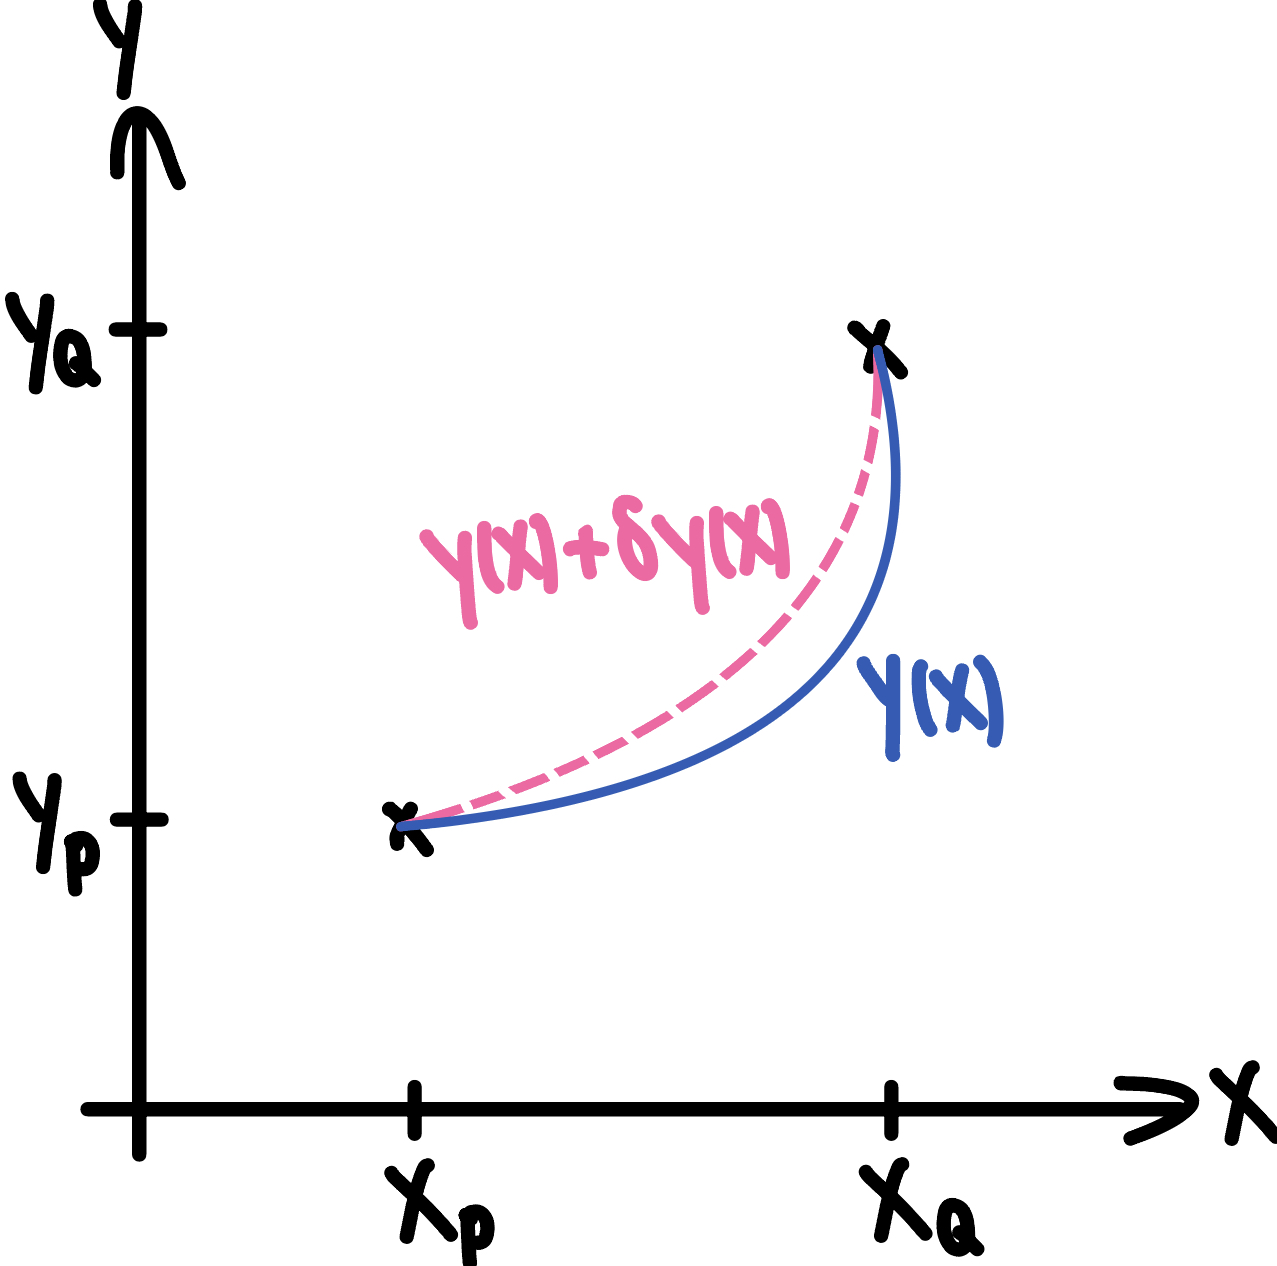
\includegraphics[width=0.3\textwidth]{Functional variation}
\end{wrapfigure}
Suppose we have two points, $(x_{P}, y_{P})$ and $(x_{Q}, y_{Q})$. We first a general path satisfying $y(x_{P})=y_{P}$ and $y(x_{Q})=y_{Q}$, and vary the path $y(x)\to y(x)+\d y(x)$, where $\d y$ is an infinitesimal function. The two points $(x_{P}, y_{P})$ and $(x_{Q}, y_{Q})$ are fixed, so the boundary conditions $\d y(x_{P})=\d y(x_{Q})=0$ are needed.\bigskip\newline
The time of the new path is $T[y+\d y]$, and the functional variation is
\begin{align*}
\d T\equiv T[y+\d y]-T[y]
\end{align*}

\begin{example}[Light propagation in the vacuum]
The propagation time between two points is
\begin{eqnbox}
\begin{align}
T=\frac{1}{c}\int_{x_{P}}^{x_{Q}}\sqrt{1+{\left(\frac{dy}{dx}\right)}^{2}}\,dx
\end{align}
\end{eqnbox}
We vary $y(x)\to y(x)+\d y(x)$. By Taylor expansion,
\begin{align*}
\sqrt{1+{\left(\frac{d[y(x)+\d y(x)]}{dx}\right)}^{2}}&=\sqrt{1+\frac{dy^{2}+2dyd\d y+d(\d y)^{2}}{dx^{2}}}\\
&=\sqrt{\left(1+(y')^{2}\right)\left[1+\frac{2dyd\d y+d(\d y)^{2}}{\left(1+(y')^{2}\right)dx^{2}}\right]}\\
&\approx \sqrt{1+(y')^{2}}\left[1+\frac{1}{2}\cdot \frac{2dyd\d y+d(\d y)^{2}}{\left(1+(y')^{2}\right)dx^{2}}\right]\\
&=\sqrt{1+(y')^{2}}+\frac{y'}{\sqrt{1+(y')^{2}}}\frac{d\d y}{dx}+\bigO[(\d y)^{2}]
\end{align*}
The functional variation is thus
\begin{align*}
\d T[y]&=\frac{1}{c}\int_{x_{P}}^{x_{Q}}\frac{y'}{\sqrt{1+(y')^{2}}}\frac{d\d y}{dx}\,dx
\end{align*}
Let $u=\frac{y'}{\sqrt{1+(y')^{2}}}$ and $v=\d y$. Using integration by parts,
\begin{eqnbox}
\begin{align}
\d T[y]&=\frac{1}{c}\int_{x_{P}}^{x_{Q}}\left[\frac{d}{dx}\left(\frac{y'}{\sqrt{1+(y')^{2}}}\d y\right)-\d y\frac{d}{dx}\left(\frac{y'}{\sqrt{1+(y')^{2}}}\right)\right]\,dx\nonumber\\
&=-\frac{1}{c}\int_{x_{P}}^{x_{Q}}\d y\frac{d}{dx}\left(\frac{y'}{\sqrt{1+(y')^{2}}}\right)\,dx
\end{align}
\end{eqnbox}
We have dropped the total derivative term since $\d y=0$ on the boundary. $\d T=0$ for all $\d y$, therefore
\begin{eqnbox}
\begin{align}
\frac{d}{dx}\left(\frac{y'}{\sqrt{1+(y')^{2}}}\right)=0\implies y'\text{ is constant}
\end{align}
\end{eqnbox}
This implies light travels with straight lines.
\end{example}

\section{Principle of extremal action}
The action principle states that for a theory defined by an action $S$, the equation of motion of the theory corresponds to the extremal action $\d S=0$.
\begin{example}[Newton's second law derived from action]
Consider a potential $V(q)$, where $q(t)$ is the position of the particle. In Newtonian mechanics, the action is
\begin{eqnbox}
\begin{align}
S[q]=\int_{t_{1}}^{t_{2}}\left[\frac{1}{2}m\dot{q}^{2}-V(q)\right]\,dt
\end{align}
\end{eqnbox}
eq. (7.4) has the form of integrating $T-V$ over time, where $T$ is the kinetic energy and $V$ is the potential energy. Similar to studying how light propagates in the vacuum, we vary $q(t)\to q(t)+\d q(t)$ and keep $\d q(t_{1})=\d q(t_{2})=0$.
\begin{align*}
\frac{1}{2}m{\left(\dot{q}+\d \dot{q}\right)}^{2}-V(q+\d q)&=\frac{1}{2}m\dot{q}^{2}+m\dot{q}\d \dot{q}+\frac{1}{2}m\d \dot{q}^{2}-V(q)-\frac{dV}{dq}\d q\\
\implies \frac{1}{2}m{\left(\dot{q}+\d \dot{q}\right)}^{2}-V(q+\d q)-\left[\frac{1}{2}m\dot{q}^{2}-V(q)\right]&=m\dot{q}\d \dot{q}-\frac{dV}{dq}\d q+\bigO(\d \dot{q}^{2})
\end{align*}
An infinitesimal change of the action is thus
\begin{eqnbox}
\begin{align}
\d S&=\int_{t_{1}}^{t_{2}}\left(m\dot{q}\d \dot{q}-\frac{dV}{dq}\d q\right)\,dt\nonumber\\
&=\int_{t_{1}}^{t_{2}}\left[\frac{d}{dt}\left(m\dot{q}\d q\right)-m\ddot{q}\d q-\frac{dV}{dq}\d q\right]\,dt\nonumber\\
&=\int_{t_{1}}^{t_{2}}\left(-m\ddot{q}-\frac{dV}{dq}\right)\d q\,dt
\end{align}
\end{eqnbox}
Again, we have dropped the boundary term. $\d S=0$ for all $\d q$, so the equation of motion is
\begin{eqnbox}
\begin{align}
m\ddot{q}+\frac{dV}{dq}=0
\end{align}
\end{eqnbox}
We have re-derived Newton's second law of motion.
\end{example}

\subsection*{Integration by parts}
You might feel puzzled about how to obtain $\frac{d}{dt}(m\dot{q}\d q)-m\ddot{q}\d q$ from $m\dot{q}\d\dot{q}$ in eq. (7.5) above. If so, you have come to the right place. This is simply integration by parts, or equivalently, the product rule in reverse, which you should have learnt in high school. This technique will be applied extensively throughout this chapter.\bigskip\newline
Suppose we have two differentiable functions $f(x)$ and $g(x)$, the product rule states that the derivative of their product is
\begin{align*}
\frac{d}{dx}(fg)=\frac{df}{dx}\cdot g+f\cdot\frac{dg}{dx}
\end{align*}
and sometimes it is convenient to switch the orders
\begin{align*}
\frac{df}{dx}\cdot g=\frac{d}{dx}(fg)-f\cdot\frac{dg}{dx}
\end{align*}
In the previous example, we want to extract $\d q$ from the integral of $\d S$. We notice that
\begin{align*}
\frac{d}{dt}(m\dot{q}\d q)=m\ddot{q}\d q+m\dot{q}\d \dot{q}\iff m\dot{q}\d\dot{q}=\frac{d}{dt}(m\dot{q}\d q)-m\ddot{q}\d q
\end{align*}
This is how we rewrite $m\dot{q}\d\dot{q}$ in terms of $\d q$ and then drop the boundary term $\frac{d}{dt}(m\dot{q}\d q)$.\bigskip\newline
It is straightforward to generalize this technique to a product of three or more functions. In the case of three functions,
\begin{align*}
\frac{df}{dx}\cdot gh=\frac{d}{dx}(fgh)-f\cdot\frac{dg}{dx}\cdot h-fg\cdot\frac{dh}{dx}
\end{align*}
and for some problems you may even have to apply this technique more than once to extract $\d q$ completely, e.g. see \hyperref[Action principle of Galileons]{2019-20 Fall Midterm Q5 - Action principle of Galileons} and \hyperref[A strange particle with a strange Lagrangian]{2022-23 Fall Final Q3 - A strange particle with a strange Lagrangian}.
\subsection*{Euler-Lagrange equation}
Consider the Lagrangian $\La (q_{i}, \dot{q}_{i}, t)$ of a particle. The action is defined as
\begin{eqnbox}
\begin{align}
S=\int \La(q_{i}, \dot{q}_{i}, t)\,dt
\end{align}
\end{eqnbox}
By the method of variation, 
\begin{align*}
\d S&=\sum_{i}\int\left(\frac{\p \La}{\p q_{i}}\d q_{i}+\frac{\p \La}{\p \dot{q}_{i}}\d\dot{q}_{i}\right)\,dt\\
&=\sum_{i}\int\left[\frac{\p \La}{\p q_{i}}\d q_{i}+\frac{d}{dt}\left(\frac{\p \La}{\p \dot{q}_{i}}\d q_{i}\right)-\frac{d}{dt}\left(\frac{\p \La}{\p \dot{q}_{i}}\right)\d q_{i}\right]\,dt\\
&=\sum_{i}\int\left[\frac{\p \La}{\p q_{i}}-\frac{d}{dt}\left(\frac{\p \La}{\p \dot{q}_{i}}\right)\right]\d q_{i}\,dt
\end{align*}
We have dropped the boundary term in the last step. $\d S=0$ for all $\d q$, so we arrive at the Euler-Lagrange equation.
\begin{eqnbox}
\begin{align}
\frac{\p \La}{\p q_{i}}-\frac{d}{dt}\left(\frac{\p \La}{\p \dot{q}_{i}}\right)=0
\end{align}
\end{eqnbox}

\subsection*{Generalized Euler-Lagrange equation}
If the Lagrangian contains higher order time derivatives, i.e. the second time derivative $\ddot{q}$ and beyond, the usual Euler-Lagrange equation is not applicable. Instead, the generalized version shown below has to be used,
\begin{align*}
\frac{\p \La}{\p q}+\sum_{n=1}(-1)^{n}\frac{d^{n}}{dt^{n}}\frac{\p \La}{\p (d^{n}q/dt^{n})}=0
\end{align*}
The derivation can be found at \hyperref[A strange particle with a strange Lagrangian]{2022-23 Fall Final Q3 - A strange particle with a strange Lagrangian}. When $n=1$, it is reduced to eq. (7.8).

\section{Symmetry}
A symmetry of a theory is a transformation under which the theory does not change. Consider an infinitesimal transformation $q_{i}\to \tilde{q}_{i}=q_{i}+\e\d q_{i}$, where $\e$ is an infinitesimal constant. If the action does not change, 
\begin{eqnbox}
\begin{align}
\d S=\int \La(\tilde{q}_{i}, \dot{\tilde{q}}_{i}, t)\,dt-\int \La(q_{i}, \dot{q}_{i}, t)\,dt=0
\end{align}
\end{eqnbox}
then the transformation is a symmetry.

\begin{example}[Time translation symmetry]
Time translation can be written as
\begin{eqnbox}
\begin{align}
q_{i}(t)\to\tilde{q}_{i}(t)=q_{i}(t+\e\d t)=q_{i}(t)+\e \dot{q}_{i}(t)\d t
\end{align}
\end{eqnbox}
Therefore,
\begin{eqnbox}
\begin{align}
\d q_{i}=\dot{q}_{i}\d t\implies \d \dot{q}_{i}=\ddot{q}_{i}\d t
\end{align}
\end{eqnbox}
If the Lagrangian $\La$ has no explicit time dependence, i.e. $\La(q_{i}, \dot{q}_{i}, t)=\La(q_{i}, \dot{q}_{i})$, 
\begin{eqnbox}
\begin{align}
\d \La&=\left(\frac{\p \La}{\p q_{i}}\dot{q}_{i}+\frac{\p \La}{\p \dot{q}_{i}}\ddot{q}_{i}\right)\e\d t\nonumber\\
&=\left(\frac{\p \La}{\p q_{i}}\d q_{i}+\frac{\p \La}{\p \dot{q}_{i}}\d \dot{q}_{i}\right)\e\nonumber\\
&=\e\frac{d\left(\La\d t\right)}{dt}
\end{align}
\end{eqnbox}
$\d \La$ is a total time derivative, so we have $\d S=0$, which means time translation is a symmetry for $\La$ with no explicit time dependence.
\end{example}

\section{Conservation laws}
Let's assume the transformation $q_{i}\to\tilde{q}_{i}=q_{i}+\e\d q_{i}$ is a symmetry. Using the variation principle,
\begin{align*}
\d L&=\sum_{i}\left(\frac{\p \La}{\p q_{i}}\e\d q_{i}+\frac{\p \La}{\p q_{i}}\e\d \dot{q}_{i}\right)\\
&=\sum_{i}\left[\frac{\p \La}{\p q_{i}}\e\d q_{i}+\frac{d}{dt}\left(\frac{\p \La}{\p \dot{q}_{i}}\e\d q_{i}\right)-\frac{d}{dt}\left(\frac{\p \La}{\p \dot{q}_{i}}\right)\e\d q_{i}\right]\\
&=\e\sum_{i}\left[\frac{\p \La}{\p q_{i}}\d q_{i}-\frac{d}{dt}\left(\frac{\p \La}{\p \dot{q}_{i}}\right)\d q_{i}+\frac{d}{dt}\left(\frac{\p \La}{\p \dot{q}_{i}}\d q_{i}\right)\right]
\end{align*}
By the Euler-Lagrange equation, the first two terms in the summation cancel out, so
\begin{align*}
\d L=\e\sum_{i}\frac{d}{dt}\left(\frac{\p \La}{\p \dot{q}_{i}}\d q_{i}\right)
\end{align*}
Meanwhile, we know that a symmetry leaves the action invariant and changes the Lagrangian by at most a total time derivative,
\begin{align*}
\d L=-\e\frac{dg}{dt}
\end{align*}
where $g$ is some quantity. Combining these two lines,
\begin{align*}
\e\sum_{i}\frac{d}{dt}\left(\frac{\p \La}{\p \dot{q}_{i}}\d q_{i}\right)&=-\e\frac{dg}{dt}\\
\implies \e\frac{d}{dt}\left(g+\sum_{i}\frac{\p \La}{\p \dot{q}_{i}}\d q_{i}\right)&=0
\end{align*}
Therefore, as a result of the symmetry, the quantity
\begin{eqnbox}
\begin{align}
Q=g+\sum_{i}\frac{\p \La}{\p \dot{q}_{i}}\d q_{i}
\end{align}
\end{eqnbox}
is conserved, i.e. $\dot{Q}=0$.

\begin{example}[Time translation symmetry and energy conservation]
Under time translation, $\d q_{i}=\dot{q}_{i}\d t$, and from eq. (7.12) we have $g=-\La \d t$. The conserved quantity is
\begin{align*}
Q=-\La \d t+\sum_{i}\frac{\p \La}{\p \dot{q}_{i}}\dot{q}_{i}\d t
\end{align*}
The Hamiltonian is thus a conserved quantity,
\begin{eqnbox}
\begin{align}
H\equiv\frac{Q}{\d t}=\sum_{i}\frac{\p \La}{\p \dot{q}_{i}}\dot{q}_{i}-\La
\end{align}
\end{eqnbox}
We can write down the Lagrangian in Newtonian mechanics explicitly,
\begin{eqnbox}
\begin{align}
\La=\sum_{i}\frac{1}{2}\dot{q}_{i}^{2}-V(q_{1}, q_{2}, \dots, q_{n})
\end{align}
\end{eqnbox}
Putting eq. (7.15) into eq. (7.14),
\begin{eqnbox}
\begin{align}
H&=\sum_{i}\dot{q}_{i}^{2}-\La\nonumber\\
&=\sum_{i}\frac{1}{2}\dot{q}_{i}^{2}+V(q_{1}, q_{2}, \dots, q_{n})
\end{align}
\end{eqnbox}
The conserved Hamiltonian is the energy of the system. Time translation symmetry corresponds to conservation of energy.
\end{example}

\addcontentsline{toc}{section}{Problems}
\section*{Problems}
\begin{problem}
Use the Euler-Lagrange equation to derive the Newton's second law for a particle moving in a potential.
\end{problem}

\begin{solbox}
The Lagrangian in Newtonian mechanics is
\begin{align*}
\La=\frac{1}{2}m\dot{q}^{2}-V(q)
\end{align*}
and the Euler-Lagrange equation is
\begin{align*}
\frac{\p \La}{\p q}-\frac{d}{dt}\left(\frac{\p \La}{\p \dot{q}}\right)=0
\end{align*}
After substitution,
\begin{align*}
-\frac{dV}{dq}-\frac{d}{dt}\left(m\dot{q}\right)&=0\\
m\ddot{q}+\frac{dV}{dq}&=0
\end{align*}
This is the Newton's second law.
\end{solbox}

\begin{problem}
The action of a freely moving relativistic particle is
\begin{align*}
S=\a \int d\t=\a \int\sqrt{1-\frac{\dot{q}^{2}}{c^{2}}}\,dt
\end{align*}
a) Determine the value of $\a$ by taking the Newtonian limit $\dot{q}\ll c$.\bigskip\newline
b) Show that the system has time translation symmetry.\bigskip\newline
c) Derive the relativistic energy as the conserved quantity of time translation.\bigskip\newline
d) Show that the system has space translation symmetry $q(t)\to q(t)+\e$.\bigskip\newline
e) Derive the conserved quantity of space translation.
\end{problem}

\begin{solbox}
a) By Taylor expansion,
\begin{align*}
S=\a \int\sqrt{1-\frac{\dot{q}^{2}}{c^{2}}}\,dt\approx \a \int\left(1-\frac{1}{2}\frac{\dot{q}^{2}}{c^{2}}\right)\,dt
\end{align*}
Comparing with the Lagrangian in Newtonian mechanics, $\La=\frac{1}{2}m\dot{q}^{2}$, we know $\a=-mc^{2}$.\bigskip\newline
b) Time translation can be written as $q(t)\to q(t)+\e \dot{q}(t)\d t$, so $\d q=\dot{q}\d t\implies \d \dot{q}=\ddot{q}\d t$.
\begin{align*}
\sqrt{1-\frac{\left(\dot{q}+\e\d\dot{q}\right)^{2}}{c^{2}}}&=\sqrt{1-\frac{\dot{q}^{2}+2\e\dot{q}\d\dot{q}+\e^{2}\d\dot{q}^{2}}{c^{2}}}\\
&=\sqrt{\left(1-\frac{\dot{q}^{2}}{c^{2}}\right)\left[1-\frac{2\e\dot{q}\d\dot{q}+\e^{2}\d\dot{q}^{2}}{\left(1-\frac{\dot{q}^{2}}{c^{2}}\right)c^{2}}\right]}\\
&\approx \sqrt{1-\frac{\dot{q}^{2}}{c^{2}}}\left[1-\frac{1}{2}\cdot\frac{2\e\dot{q}\d\dot{q}+\e^{2}\d\dot{q}^{2}}{\left(1-\frac{\dot{q}^{2}}{c^{2}}\right)c^{2}}\right]\\
&=\sqrt{1-\frac{\dot{q}^{2}}{c^{2}}}-\frac{\e\dot{q}\d\dot{q}}{c^{2}\sqrt{1-\frac{\dot{q}^{2}}{c^{2}}}}+\bigO\left(\d\dot{q}^{2}\right)\\
\implies \d S&=-mc^{2}\cdot -\e\int\frac{\dot{q}\d\dot{q}}{c^{2}\sqrt{1-\frac{\dot{q}^{2}}{c^{2}}}}\,dt\\
&=\e\int\frac{m\dot{q}\ddot{q}\d t}{\sqrt{1-\frac{\dot{q}^{2}}{c^{2}}}}\,dt
\end{align*}
Note that 
\begin{align*}
\frac{d}{dt}\left(-\sqrt{1-\frac{\dot{q}^{2}}{c^{2}}}\d t\right)=\frac{1}{c^{2}}\left(1-\frac{\dot{q}^{2}}{c^{2}}\right)^{-\frac{1}{2}}\dot{q}\ddot{q}\d t
\end{align*}
so
\begin{align*}
\d S&=\e mc^{2}\int\frac{d}{dt}\left(-\sqrt{1-\frac{\dot{q}^{2}}{c^{2}}}\d t\right)\,dt=0
\end{align*}
We have dropped the total derivative term. The system has time translation symmetry.\bigskip\newline
c) From (b), we have $g=mc^{2}\sqrt{1-\frac{\dot{q}^{2}}{c^{2}}}\d t$. The conserved quantity is
\begin{align*}
Q&=g+\frac{\p \La}{\p \dot{q}}\d q\\
&=mc^{2}\sqrt{1-\frac{\dot{q}^{2}}{c^{2}}}\d t+\frac{m\dot{q}^{2}}{\sqrt{1-\frac{\dot{q}^{2}}{c^{2}}}}\d t\\
&=\frac{mc^{2}\left(1-\frac{\dot{q}^{2}}{c^{2}}\right)+m\dot{q}^{2}}{\sqrt{1-\frac{\dot{q}^{2}}{c^{2}}}}\d t\\
&=\c mc^{2}\d t
\end{align*}
The relativistic energy is thus conserved,
\begin{align*}
E=\c mc^{2}=\frac{Q}{\d t}
\end{align*}
d) Space translation is $q(t)\to q(t)+\e$, so $\dot{q}$ remains unchanged and $\d S=0$. This implies space translation is a symmetry.\bigskip\newline
e) The conserved quantity is
\begin{align*}
Q&=g+\frac{\p \La}{\p \dot{q}}\d q\\
&=0-mc^{2}\cdot\frac{1}{2}{\left(1-\frac{\dot{q}^{2}}{c^{2}}\right)}^{-\frac{1}{2}}\cdot-\frac{2\dot{q}}{c^{2}}\\
&=\c m\dot{q}
\end{align*}
This is the relativistic momentum.
\end{solbox}

\subsection*{2019-20 Fall Midterm Q5 - Action principle of Galileons}
\label{Action principle of Galileons}
There are some very special theories, in which the equation of motion can be derived from variation principle, but not the Euler-Lagrange equation. For example, consider a (simplified version of) Galileon action:
\begin{align*}
S=\int \left[\ddot{q}\dot{q}q-V(q)\right]\,dt
\end{align*}
Use variation principle to derive its equation of motion, and show that the result is different from that obtained from the Euler-Lagrange equation.

\begin{solbox}
Using the variation principle, $q\to q+\d q$, $\dot{q}\to \dot{q}+\d \dot{q}$ and $\ddot{q}\to \ddot{q}+\d\ddot{q}$.
\begin{align*}
\d \La&=\left(\ddot{q}+\d\ddot{q}\right)\left(\dot{q}+\d\dot{q}\right)\left(q+\d q\right)-V(q+\d q)-\left[\ddot{q}\dot{q}q-V(q)\right]\\
&=\d\ddot{q}\dot{q}q+\ddot{q}\d\dot{q}q+\ddot{q}\dot{q}\d q-V'(q)\d q\\
\d \ddot{q}\dot{q}q&=\frac{d}{dt}\left(\d\dot{q}\dot{q}q\right)-\d\dot{q}\ddot{q}q-\d\dot{q}\dot{q}^{2}\\
&=\frac{d}{dt}\left(\d\dot{q}\dot{q}q\right)-\left[\frac{d}{dt}\left(\d q\ddot{q}q\right)-\d q \dddot{q} q-\d q\ddot{q}\dot{q}\right]-\left[\frac{d}{dt}\left(\d q\dot{q}^{2}\right)-\d q\cdot2\dot{q}\ddot{q}\right]\\
&=\d q\left(3\ddot{q}\dot{q}+\dddot{q}q\right)+\frac{d}{dt}\left(\d\dot{q}\dot{q}q\right)-\frac{d}{dt}\left(\d q\ddot{q}q\right)-\frac{d}{dt}\left(\d q\dot{q}^{2}\right)\\
\ddot{q}\d \dot{q}q&=\frac{d}{dt}\left(\ddot{q}\d q q\right)-\dddot{q}\d q q-\ddot{q}\d q\dot{q}\\
&=\d q\left(-\dddot{q}q-\ddot{q}\dot{q}\right)+\frac{d}{dt}\left(\ddot{q}\d q q\right)
\end{align*}
After substitution,
\begin{align*}
\d S&=\int\left[\d q\left(3\ddot{q}\dot{q}+\dddot{q}q\right)+\d q\left(-\dddot{q}q-\ddot{q}\dot{q}\right)+\ddot{q}\dot{q}\d q-V'(q)\d q\right]\,dt\\
&=\int\left[3\ddot{q}\dot{q}-V'(q)\right]\d q\,dt
\end{align*}
We have dropped the total derivative terms. $\d S=0$ for all $\d q$, so the equation of motion is
\begin{align*}
3\ddot{q}\dot{q}-V'(q)=0
\end{align*}
From the action, the Lagrangian is
\begin{align*}
\La=\ddot{q}\dot{q}q-V(q)
\end{align*}
Putting it into the Euler-Lagrange equation,
\begin{align*}
\frac{\p \La}{\p q}-\frac{d}{dt}\left(\frac{\p \La}{\p \dot{q}}\right)=\ddot{q}\dot{q}-V'(q)-\frac{d}{dt}\left(\ddot{q}q\right)&=0\\
\ddot{q}\dot{q}-V'(q)-\dddot{q}q-\ddot{q}\dot{q}&=0\\
\dddot{q}q+V'(q)&=0
\end{align*}
The result is different from that obtained from the variation principle. It is because the Lagrangian contains the second time derivative $\ddot{q}$. Using the generalized version of the Euler-Lagrange equation indeed gives the correct result.
\end{solbox}

\subsection*{2020-21 Fall Final Q5 - Action principle with constraints}
Consider the action for $q_{1}(t)$ and $q_{2}(t)$:
\begin{align*}
S=\int\left(\dot{q}_{1}^{2}-q_{1}^{2}+q_{1}\dot{q}_{2}-q_{2}^{2}\right)\,dt
\end{align*}
a) Note that there is no $\dot{q}_{2}^{2}$ term in the Lagrangian. Do an integration by part to further eliminate $\dot{q}_{2}$ from the Lagrangian (assuming that boundary terms can be dropped).\bigskip\newline
b) Use variation principle $q_{2}\to q_{2}+\d q_{2}$ to solve $q_{2}$. Insert the solution back to the Lagrangian, to obtain an action of $q_{1}$.\bigskip\newline
c) Derive the equation of motion of $q_{1}$ (which does not involve $q_{2}$).

\begin{solbox}
a) Using integration by parts,
\begin{align*}
q_{1}\dot{q}_{2}&=\frac{d}{dt}\left(q_{1}q_{2}\right)-\dot{q}_{1}q_{2}\\
\implies S&=\int\left(\dot{q}_{1}^{2}-q_{1}^{2}-\dot{q}_{1}q_{2}-q_{2}^{2}\right)\,dt
\end{align*}
We have dropped the boundary term.\bigskip\newline
b) Using the variation principle, $q_{2}\to q_{2}+\d q_{2}$.
\begin{align*}
\d S&=\int\left(-\dot{q}_{1}\d q_{2}-2q_{2}\d q_{2}\right)\,dt\\
&=\int \left(-\dot{q}_{1}-2q_{2}\right)\d q_{2}\,dt
\end{align*}
$\d S=0$ for all $\d q_{2}$, so
\begin{align*}
-\dot{q}_{1}-2q_{2}&=0\\
q_{2}&=-\frac{\dot{q}_{1}}{2}
\end{align*}
Inserting $q_{2}=-\frac{\dot{q}_{1}}{2}$ into the action yields
\begin{align*}
S&=\int\left(\frac{5}{4}\dot{q}_{1}^{2}-q_{1}^{2}\right)\,dt
\end{align*}
c) From the action, the Lagrangian is
\begin{align*}
\La=\frac{5}{4}\dot{q}_{1}^{2}-q_{1}^{2}
\end{align*}
Putting it into the Euler-Lagrange equation,
\begin{align*}
\frac{\p \La}{\p q}-\frac{d}{dt}\left(\frac{\p \La}{\p \dot{q}}\right)=-2q_{1}-\frac{d}{dt}\left(\frac{5}{2}\dot{q}_{1}\right)&=0\\
-2q_{1}-\frac{5}{2}\ddot{q}_{1}&=0\\
5\ddot{q}_{1}+4q_{1}&=0
\end{align*}
\end{solbox}

\subsection*{2021-22 Fall Final Q4 - A cosmological scalar field}
In cosmology, a homogeneous and isotropic scalar field has an action
\begin{align*}
S=\int dt\,a^{3}(t)\left[\frac{1}{2}\dot{\phi}^{2}-V(\phi)\right]
\end{align*}
where $a(t)$ is a function of time, and $V(\phi)$ is a function of $\phi$.\bigskip\newline
a) Derive the equation of motion of $\phi$.\bigskip\newline
b) When $V=0$, this scalar field has a symmetry $\phi(t)\to \tilde{\phi}(t)=\phi(t)+\e$, where $\e$ is a constant. Derive the corresponding conserved quantity.

\begin{solbox}
a) From the action, the Lagrangian is
\begin{align*}
\La=a^{3}(t)\left[\frac{1}{2}\dot{\phi}^{2}-V(\phi)\right]
\end{align*}
Substituting into the Euler-Lagrange equation,
\begin{align*}
\frac{\p \La}{\p \phi}-\frac{d}{dt}\left(\frac{\p \La}{\p \dot{\phi}}\right)=-a^{3}\frac{dV}{d\phi}-\frac{d}{dt}\left(a^{3}\dot{\phi}\right)&=0\\
-a^{3}\frac{dV}{d\phi}-\left(3a^{2}\dot{a}\dot{\phi}+a^{3}\ddot{\phi}\right)&=0\\
\ddot{\phi}+\frac{3\dot{a}}{a}\dot{\phi}+\frac{dV}{d\phi}&=0
\end{align*}
Since $H\equiv\frac{\dot{a}}{a}$, the equation of motion is
\begin{align*}
\ddot{\phi}+3H\dot{\phi}+\frac{dV}{d\phi}=0
\end{align*}
b) When $V=0$, the action becomes
\begin{align*}
S=\int dt\,a^{3}(t)\frac{1}{2}\dot{\phi}^{2}
\end{align*}
Under the shift $\phi\to\phi+\e$, $\dot{\phi}$ remains unchanged. The change in action is
\begin{align*}
\d S=\int a^{3}(t)\dot{\phi}\cdot0=0
\end{align*}
We prove that $\phi(t)\to \tilde{\phi}(t)=\phi(t)+\e$ is a symmetry, and find that $g=0$. The conserved quantity is
\begin{align*}
Q&=g+\frac{\p \La}{\p \dot{\phi}}\d \phi\\
&=0+a^{3}(t)\dot{\phi}\\
&=a^{3}(t)\dot{\phi}
\end{align*}
\end{solbox}

\subsection*{2022-23 Fall Final Q3 - A strange particle with a strange Lagrangian}
\label{A strange particle with a strange Lagrangian}
Consider a strange particle with Lagrangian $\mathlarger{\La=\sum_{n=0}^{N}c_{n}\frac{d^{n}q}{dt^{n}}}$.\bigskip\newline
a) Can its equation of motion be derived from the Euler-Lagrange equation? Briefly explain the reason use one sentence.\bigskip\newline
b) Derive its equation of motion from the variation principle.

\begin{solbox}
a) No, since it contains higher order time derivatives, i.e. $\frac{d^{n}q}{dt^{n}}$ with $n\geq2$.\bigskip\newline
b) From the Lagrangian, the action is
\begin{align*}
    S=\int \La dt=\int \sum_{n=0}^{N}c_{n}\frac{d^{n}q}{dt^{n}}dt
\end{align*}
Using the variation principle, $\frac{d^{n}q}{dt^{n}}\to\frac{d^{n}q}{dt^{n}}+\d\left(\frac{d^{n}q}{dt^{n}}\right)$.
\begin{align*}
\d\La&=\sum_{n=0}^{N}\frac{\d\La}{\d(d^{n}q/dt^{n})}\d\left(\frac{d^{n}q}{dt^{n}}\right)
\end{align*}
Using integration by parts,
\begin{align*}
\frac{\d\La}{\d\dot{q}}\d\dot{q}&=\frac{d}{dt}\left(\frac{\d\La}{\d\dot{q}}\d q\right)-\frac{d}{dt}\left(\frac{\d\La}{\d\dot{q}}\right)\d q\\
\frac{\d\La}{\d\ddot{q}}\d\ddot{q}&=\frac{d}{dt}\left(\frac{\d\La}{\d\ddot{q}}\d\dot{q}\right)-\frac{d}{dt}\left(\frac{\d\La}{\d\ddot{q}}\right)\d\dot{q}\\
&=\frac{d}{dt}\left(\frac{\d\La}{\d\ddot{q}}\d\dot{q}\right)-\left[\frac{d}{dt}\left(\frac{d}{dt}\left(\frac{\d\La}{\d\ddot{q}}\right)\d q\right)-\frac{d^{2}}{dt^{2}}\left(\frac{\d\La}{\d\ddot{q}}\right)\d q\right]\\
&=\frac{d}{dt}\left(\frac{\d\La}{\d\ddot{q}}\d\dot{q}\right)-\frac{d}{dt}\left(\frac{d}{dt}\left(\frac{\d\La}{\d\ddot{q}}\right)\d q\right)+(-1)^{2}\frac{d^{2}}{dt^{2}}\left(\frac{\d\La}{\d\ddot{q}}\right)\d q
\end{align*}
It is straightforward to generalize this calculation to higher order derivatives. When we extract $\d q$ from $\frac{\d\La}{\d\ddot{q}}\d\ddot{q}$, we perform integration by parts twice. Each time, an extra factor of -1 emerges, the $\frac{\d\La}{\d\ddot{q}}$ is differentiated once and the order in $\d\ddot{q}$ decreases by 1.\bigskip\newline
For an arbitrary $n$, we do integration by parts $n$ times,
\begin{align*}
\begin{split}
\frac{\d\La}{\d(d^{n}q/dt^{n})}\d\left(\frac{d^{n}q}{dt^{n}}\right)&=\frac{d}{dt}\left(\frac{\d\La}{\d(d^{n}q/dt^{n})}\d\left(\frac{d^{n-1}q}{dt^{n-1}}\right)\right)-\frac{d}{dt}\left(\frac{\d\La}{\d(d^{n}q/dt^{n})}\right)\d\left(\frac{d^{n-1}q}{dt^{n-1}}\right)\\
&=\frac{d}{dt}\left(\frac{\d\La}{\d(d^{n}q/dt^{n})}\d\left(\frac{d^{n-1}q}{dt^{n-1}}\right)\right)-\left[\frac{d}{dt}\left(\frac{d}{dt}\left(\frac{\d\La}{\d(d^{n}q/dt^{n})}\right)\d\left(\frac{d^{n-2}q}{dt^{n-2}}\right)\right)\right.\\
&\left.\,\,\,\,\,-\frac{d^{2}}{dt^{2}}\left(\frac{\d\La}{\d(d^{n}q/dt^{n})}\right)\d\left(\frac{d^{n-2}q}{dt^{n-2}}\right)\right]
\end{split}
\end{align*}
\begin{align*}
&=\cdots\\
&=(\textrm{boundary terms})+(-1)^{n}\frac{d^{n}}{dt^{n}}\left(\frac{\d\La}{\d(d^{n}q/dt^{n})}\right)\d q
\end{align*}
Hence, the change in action is
\begin{align*}
\d S=\int\left[\sum_{n=0}^{N}(-1)^{n}\frac{d^{n}}{dt^{n}}\left(\frac{\d\La}{\d(d^{n}q/dt^{n})}\right)\right]\d q\,dt
\end{align*}
$\d S=0$ for all $\d q$, so
\begin{align*}
\sum_{n=0}^{N}(-1)^{n}\frac{d^{n}}{dt^{n}}\left(\frac{\d\La}{\d(d^{n}q/dt^{n})}\right)=0
\end{align*}
We have derived the generalized Euler-Lagrange equation. Substituting the Lagrangian into it, the equation of motion is
\begin{align*}
\sum_{n=0}^{N}(-1)^{n}\frac{d^{n}c_{n}}{dt^{n}}=0
\end{align*}
(This is perhaps the most difficult exam question on the action principle so far. Students are required to generalize the method of integration by parts to higher order time derivatives.)
\end{solbox}

\newpage
\chapterimage{Chapter 8} % Chapter heading image
\chapter{Entropy}
For an isolated system consisting of $n$ subsystems, define
\begin{eqnbox}
\begin{align}
\D S_{i}=\frac{\D Q_{i}}{T}
\end{align}
\end{eqnbox}
 for each subsystem $i$, where $\D Q_{i}$ is the heat flowing into the subsystem if the process is reversible. The second law of thermodynamics states that
\begin{eqnbox}
\begin{align}
\D S=\sum_{i=1}^{n}\D S_{n}\geq 0
\end{align}
\end{eqnbox}
The equal sign is taken for reversible process, and for irreversible process $\D S>0$.

\section{Statistical entropy}
Consider an isolated system consisting of two subsystems, A and B, which have fixed volume and can exchange heat. The total energy $E=E_{A}+E_{B}$ is fixed, while $A$ and $B$ are in thermal equilibrium, so A and B have the same temperature $T$.\bigskip\newline
The first law of thermodynamic states that $dE=TdS-pdV$, and fixed volume means $dV=0$, hence
\begin{eqnbox}
\begin{align}
\frac{dS_{A}}{dE_{A}}=\frac{dS_{B}}{dE_{B}}=\frac{1}{T}
\end{align}
\end{eqnbox}
The two subsystems have many possible microscopic states, and we assume each microscopic state has equal chance to appear. The equilibrium state should have the partition $E$ into $E_{A}$ and $E_{B}$ that corresponds to a maximal number of microscopic states, to maximize its probability to appear.\bigskip\newline
Let $\W_{A}(E_{A})$ and $\W_{B}(E_{B})$ be the number of possible microscopic states of the subsystem A and B respectively. The total number of microscopic states is
\begin{eqnbox}
\begin{align}
\W=\W_{A}(E_{A})\times\W_{B}(E_{B})
\end{align}
\end{eqnbox}
For $\W$ to be extremal we need $\frac{d\W}{dE_{A}}=0$,
\begin{align*}
0&=\frac{d\W}{dE_{A}}\\
&=\W_{B}\frac{d\W_{A}}{dE_{A}}+\W_{A}\frac{d\W_{B}}{dE_{A}}\\
&=\W_{B}\frac{d\W_{A}}{dE_{A}}+\W_{A}\frac{d\W_{B}}{dE_{B}}\frac{dE_{B}}{dE_{A}}
\end{align*}
Substitute $E_{B}=E-E_{A}$,
\begin{align*}
\W_{B}\frac{d\W_{A}}{dE_{A}}-\W_{A}\frac{d\W_{B}}{dE_{B}}&=0\\
\end{align*}
thus
\begin{eqnbox}
\begin{align}
\frac{d\ln\W_{A}}{dE_{A}}=\frac{d\ln\W_{B}}{dE_{B}}
\end{align}
\end{eqnbox}
Comparing eq. (8.5) with eq. (8.3), we derive
\begin{eqnbox}
\begin{align}
S=k_{B}\ln\W
\end{align}
\end{eqnbox}
where $k_{B}=1.381\times10^{-23}\text{J}\text{K}^{-1}$ is the Boltzmann constant.

\section{Arrow of time}
There are a few physical effects that are not time reversal invariant. They can be treated as arrows of time.

\subsection*{Thermodynamic arrow of time}
Some arrows of time are originated from the increase of thermodynamic entropy, including
\begin{itembox}
\begin{itemize}
\item Collapse of wave function after measurement. 
\item Radiation of charge propagates to the future.
\item Waves propagate forward in time.
\end{itemize}
\end{itembox}

\subsection*{Other origins}
The following arrows of time are not related to the thermodynamic time arrow.
\begin{itembox}
\begin{itemize}
\item Classical black hole absorbs but does not emit matter. According to Bekenstein and Hawking, a black hole has the highest number of microscopic states,
\begin{align*}
S=\frac{k_{B}A}{4l_{p}^{2}}
\end{align*}
where $A$ is the area of the event horizon and $l_{p}\equiv\sqrt{\frac{G\hbar}{c^{3}}}=1.616\times10^{-35}\text{m}$ is the Planck length.
\item Weak interaction.
\item Cosmological expansion.
\end{itemize}
\end{itembox}

\section{Entropy and information}
We start with an interesting thought experiment -- Maxwell's demon.

\subsection*{Maxwell's demon}
A box of equilibrium gas is separated into left and right parts, with a small gate between them. A demon known as Maxwell's demon only allows molecules with $v>v_{0}$ to enter the right part and molecules with $v<v_{0}$ to enter the left part. After some time, is the right part hotter than the left counterpart, and breaks the second law of thermodynamics?\bigskip\newline
Although heat is conducted from low temperature to high temperature, the second law of thermodynamics is not broken, since it is protected by the overwritten information in the demon's memory. The demon's brain needs to record all the molecule data and contain a huge number of possible configurations $\W_{D}$. We must as well consider the entropy of his brain $S_{D}=k_{B}\ln 2$.\bigskip\newline
If the demon has $\bigO(1)$ bits of memory only, heat must be generated in his body. To know the state of one molecule, the demon has to erase the state of the previous molecule from his memory, while erasing one bit of information generates a minimal entropy $k_{B}\ln 2$. From the first law of thermodynamics, the minimal associated heat is $k_{B}T\ln 2$.

\subsection*{Information entropy}
Information entropy is defined as the weighted average information content for all possible outcomes. Consider a set of events $X$, each event $i\in X$ has a probability $p_{i}$ to happen, then the information entropy is
\begin{eqnbox}
\begin{align}
H(X)=\sum_{i\in X}p_{i}\log_{2}\frac{1}{p_{i}}
\end{align}
\end{eqnbox}
$H(X)$ is also known as the Shannon entropy.\bigskip\newline
In statistical thermodynamics, Gibbs entropy is related to the information entropy,
\begin{align*}
S=k_{B}\ln 2\times H
\end{align*}
where $p_{i}$ is restricted to physical microscopic states.

\addcontentsline{toc}{section}{Problems}
\section*{Problems}
\begin{problem}
We fill gas into two boxes, keep the total amount of gas and temperature the same. Prove that entropy is maximized when the two boxes have equal pressure.
\end{problem}

\begin{solbox}
Consider a box with volume $V$ and gas particle number $N$. At a constant temperature, its entropy $S\sim N\ln\frac{V}{N}$. Therefore, for the entropy of two boxes,
\begin{align*}
S\sim N_{1}\ln\frac{V_{1}}{N_{1}}+N_{2}\ln\frac{V_{2}}{N_{2}}
\end{align*}
We wish to maximize $S$ with $N_{1}+N_{2}=N$ and $V_{1}$, $V_{2}$ kept fixed, so we need $\frac{\p S}{N_{1}}=0$.
\begin{align*}
0&=\frac{\p S}{N_{1}}\\
&=\ln\frac{V_{1}}{N_{1}}-1-\ln\frac{V_{2}}{N-N_{1}}+1\\
&=\ln\frac{V_{1}}{N_{1}}-\ln\frac{V_{2}}{N-N_{1}}\\
\implies \ln\frac{V_{1}}{N_{1}}&=\ln \frac{V_{2}}{N-N_{1}}\\
\left(N-N_{1}\right)V_{1}&=N_{1}V_{2}\\
\frac{V_{1}}{N_{1}}&=\frac{V_{2}}{N_{2}}
\end{align*}
Using the ideal gas law $pV=Nk_{B}T$,
\begin{align*}
p_{1}=p_{2}
\end{align*}
Entropy is maximized when the pressure is equalized.
\end{solbox}

\begin{problem}
Given $12$ balls, only one of them has a different weight. We want to use the fewest measures to find out the different one using a balance. For the first measurement, how many balls should we put on the weight, and what is its corresponding information entropy?
\end{problem}

\begin{solbox}
We must put $n$ balls on both sides of the balance. There are three different possibilities.\bigskip\newline
$L<R$: Left side is lighter than the right side. The probability is $P(L<R)=\frac{n}{12}$.\bigskip\newline
$L>R$: Left side is heavier than the left side. The probability is $P(L>R)=\frac{n}{12}$.\bigskip\newline
$L=R$: Left side and right side have the same weight. This happens if the different ball is not put on the balance, so the probability is $P(L=R)=\frac{12-2n}{12}$.\bigskip\newline
The information entropy is thus
\begin{align*}
H&=\sum p_{i}\log_{2}\frac{1}{p_{i}}\\
&=\frac{n}{12}\log_{2}\frac{12}{n}+\frac{n}{12}\log_{2}\frac{12}{n}+\frac{12-2n}{12}\log_{2}\frac{12}{12-2n}
\end{align*}
The maximal value is $H=\log_{2}3$ when $n=4$.
\end{solbox}

\subsection*{2019-20 Fall Final Q4 - Information entropy}
Compute the information entropy in the strings ``666" and ``2333", respectively. When computing probabilities for characters in a string, only consider the characters which appear in that string.

\begin{solbox}
For the first string ``666", $P(``6")=1$, so
\begin{align*}
H(``666")&=\log_{2}1\\
&=0
\end{align*}
For the second string ``2333", $P(``2")=\frac{1}{4}$ and $P(``3")=\frac{3}{4}$, so
\begin{align*}
H(``2333")&=\frac{1}{4}\log_{2}4+\frac{3}{4}\log_{2}\frac{4}{3}\\
&=2-\frac{3}{4}\log_{2}3
\end{align*}
\end{solbox}

\newpage
\addcontentsline{toc}{chapter}{2022-23 Fall Mock Exam}
\chapterimage{Mock Exam}
\chapter*{2022-23 Fall Mock Exam}
\markboth{\sffamily\bfseries\normalsize2022-23 Fall Mock Exam}{}
\section*{Take a rest first}
Congratulations, you have gone through most parts of this set of revision notes! The remaining section is a mock exam paper that helps you do a final check on your understanding.\bigskip\newline
Before attempting the mock exam, you should
\begin{itembox}
\begin{itemize}
\item Be familiar with the concepts covered, especially the labelled equations.
\item If possible, follow all the derivations given in this set of notes at least once.
\end{itemize}
\end{itembox}
With regard to the mock exam,
\begin{itembox}
\begin{itemize}
\item For numerical answers, give either the exact value or 3 significant figures.
\item The calculations in the mock exam may be slightly more tedious than the real one. Be mentally prepared for it.
\item The mock exam covers all materials of the course, so it is much lengthier than the actual midterm or the final exam. Take your time to do it.
\item Do not panic if you get most of the steps correct but the final answer wrong. It is very common for Physics students, and you can still get most of the marks. Take a deep breath and move on.
\end{itemize}
\end{itembox}

\newpage
\addcontentsline{toc}{section}{Question paper}
\begin{center}
\textbf{\LARGE PHYS 2022 - 2022-23 Fall mock exam}
\rule{16.5cm}{1pt}
\end{center}
\vspace{-0.5cm}
\section*{Part I: Multiple Choice Questions (50 Points)}
1. What is the meaning of $E$ in $E=mc^{2}$, where $m$ is a constant?\\
A. Total energy\mc B. Rest energy\mc C. Kinetic energy\mc D. Potential energy\bigskip\newline
2. When I am moving in a spaceship, I do not feel my heart rate slow down compared to my watch. This is because of\\
A. the principle of relativity\mc B. the invariance of speed of light\\
C. the observer independence of physical events\mc D. the equivalence principle\bigskip\newline
3. The ladder paradox is resolved by the fact that Alice and Bob\\
A. are not in the same reference frame\mc B. have different length of ruler\\
C. have different sense of ``same time"\mc D. have different time elapsing speed\bigskip\newline\
4. Alice and Bob are inertial observers with a relative speed. Which statement is correct?\\
A. According to what Alice sees (light to her eyes), Bob slows down\\
B. According to Alice's frame time, Bob slows down\\
C. According to what Alice sees (light to her eyes), Bob speeds up\\
D. According to Alice's frame time, Bob speeds up\bigskip\newline
5. For $v_{1}=0.5c$ and $v_{2}=c$ in the same direction, what is the velocity addition of $v_{1}$ and $v_{2}$ in special relativity?\\
A. $0.5c$\mc B. $0.75c$\mc C. $c$\mc D. $1.5c$\bigskip\newline
6. Which of the following is NOT an expression of relativistic momentum?\\
A. $\c m\frac{dx}{dt}$\mc B. $m\frac{dx}{d\t}$\mc C. $mc\tanh^{-1}\left(\frac{v}{c}\right)$\mc D. $\sqrt{\frac{E^{2}}{c^{2}}-m^{2}c^{2}}$\bigskip\newline
7. Alice is moving from right to left with respect to Bob. Consider two space-like events $P$ and $Q$ with $x_{P}>x_{Q}$ in Alice's space coordinate. Which of the following is impossible?\\
A. Both Alice and Bob consider $P$ earlier than $Q$\\
B. Both Alice and Bob consider $P$ later than $Q$\\
C. Alice considers $P$ earlier than $Q$; Bob considers $P$ later than $Q$\\
D. Alice considers $P$ later than $Q$; Bob considers $P$ earlier than $Q$\bigskip\newline
8. If two events have causal relation, these two events are\\
A. space-like\mc B. time-like\mc C. space-like or light-like\mc D. time-like or light-like\bigskip\newline
9. (Advanced) In general relativity, a person standing in front of you appears slightly taller because the Earth gravity has the effect of\\
A. frame dragging\mc B. time dilation\mc C. length contraction\mc D. light bending\bigskip\newline
10. (Advanced) If gravity is not uniform, which of the following is correct?\\
A. We can apply the equivalence principle to cancel gravity everywhere\\
B. We can apply the equivalence principle to cancel gravity locally at a point\\
C. There will not be time dilation in non-uniform gravity\\
D. General relativity cannot deal with non-uniform gravity\bigskip\newline
11. (Advanced) Alice is falling into a large black hole from outside the horizon, and Bob watches the event very far away outside the horizon. Which of the following is NOT correct?\\
A. Alice reaches the black hole singularity at finite time\\
B. Alice finds nothing special when crossing the black hole horizon\\
C. Bob finds Alice being slow when she is falling towards the black hole\\
D. Bob can see that Alice reaches the black hole singularity\bigskip\newline
12. (Advanced) Now we can observe gravitational waves from merging events of two black holes. Which of the following is NOT correct?\\
A. If the masses of the two initial black holes are $36$ and $29$ solar mass respectively, then the final merged black hole should have mass equal to $65$ solar mass\\
B. The observed gravitational waves has to be emitted outside the black hole's horizon\\
C. In the vacuum, gravitational waves propagate at the speed of light\\
D. Building more than two detectors can improve the precision of locating the source of gravitational
waves in the sky\bigskip\newline
13. (Advanced) The night sky is dark, mainly because of\\
A. the finite age of the universe\mc B. the finite size of the entire universe\\
C. the finite energy density of the universe\mc D. the finite lifetime of stars\bigskip\newline
14. The quantum wave function is a wave of\\
A. probability density\mc B. probability amplitude\\
C. mechanical oscillation\mc D. mechanical oscillation amplitude\bigskip\newline
15. Which is NOT a property of a photon?\\
A. It has energy and momentum\mc B. Its wavelength can vary continuously\\
C. Its amplitude can vary continuously\mc D. It can interfere with itself\bigskip\newline
16. Which is WRONG for superposition of quantum states?\\
A. Probability distribution of the particle can be added from component states\\
B. Quantum superposition is linear\\
C. The resulting state may have indefinite momentum\\
D. The resulting state may have indefinite energy\bigskip\newline
17. Which is WRONG for quantum measurements?\\
A. A measurement can be modelled as an operator\\
B. The wave function may collapse because of the measurement\\
C. Results of multiple measurements may depend on the order of these measurements\\
D. The measured outcome may be complex-valued instead of a real number\bigskip\newline
18. Which of the following about bosons and fermions is WRONG?\\
A. Bosons represent force and fermions represent matter for fundamental particles\\
B. The wave function of multiple Bosonic identical particles is symmetric\\
C. The wave function of multiple Fermion identical particles is anti-symmetric\\
D. There can only be one fermion on each energy level of the system\bigskip\newline
19. For an infinite potential well, which of the following would break?\\
A. The wave function must be continuous\\
B. The first derivative of the wave function must be continuous\\
C. The probability amplitude interpretation of the wave function\\
D. The existence of bound states\bigskip\newline
20. Which of the following experiment indicates that the world is made of atoms?\\
A. Dalton's multiple proportions\mc B. Newton's decomposition of white light\\
C. Rutherford's $\a$-particle scattering\mc D. Young's double slit experiment\bigskip\newline
21. For which of the below elements (in their ground states), the outermost electron is not in the $\text{s}$ orbital?\\
A. Hydrogen ($\mathbf{H}$)\mc B. Helium ($\mathbf{He}$)\\
C. Carbon ($\mathbf{C}$)\mc D. Potassium ($\mathbf{K}$)\bigskip\newline
22. (Advanced) What is the result of $\s_{1}\ket{\odot}$?\\
A. $i\ket{\odot}$\mc B. $-i\ket{\otimes}$\mc C. $i\ket{\rightarrow}$\mc D. $-i\ket{\leftarrow}$\bigskip\newline
23. (Advanced) About the EPR paradox, which of the following is WRONG?\\
A. To measure each of the particle in the EPR pair individually, random result is obtained\\
B. Measurements on the pair are correlated\\
C. The correlation of the measurement is not limited by the speed of light\\
D. The nature of EPR pairs can be mimicked by a local hidden variable theory\bigskip\newline
24. (Advanced) What protects the second law of thermodynamics in the Maxwell's demon thought experiment?\\
A. Effort to lift the gate\\
B. Quantum measurement of the particle speed\\
C. Interaction between the gas particles\\
D. Overwritten information in the demon's memory\bigskip\newline
25. (Advanced) What is the information entropy of ``AAIIMST"?\\
A. $-\frac{4}{7}+\log_{2}7$\mc B. $-\frac{4}{7}+\log_{2}6$\mc C. $-\frac{8}{7}+\frac{11}{7}\log_{2}7$\mc D. $-\frac{8}{7}+\frac{11}{7}\log_{2}6$

\section*{Part II: Long Questions (50 points)}
\subsection*{1\lq Collision of two masses (5 points)}
A particle A of rest mass $m_{A}$ collides head-on with another particle B of rest mass $m_{B}$ in $1$ space direction. Before the collision, B has energy $Q$. After the collision, B still has energy $Q$, but it is moving in the opposite direction. Express the quantities below using $m_{A}$, $m_{B}$, c and Q.\bigskip\newline
a) What is the relativistic momentum of $B$ before and after the collision?\bigskip\newline
b) What is the relativistic momentum and energy of $A$ before and after the collision?\bigskip\newline
c) What is the speed of $A$ before and after the collision?

\subsection*{2\lq Lorentz transformation (12 points)}
Alice is moving with speed $0.54c$ towards Bob. Now, the distance between Alice and Bob is $L$ in Bob's frame. Let Bob's spacetime coordinate in his own frame be $(t_{B}, x_{B})=(0, 0)$, and Alice's spacetime coordinate in her own frame be $(t_{A}, x_{A})=(0, 0)$.
\begin{figure}[H]
\centering
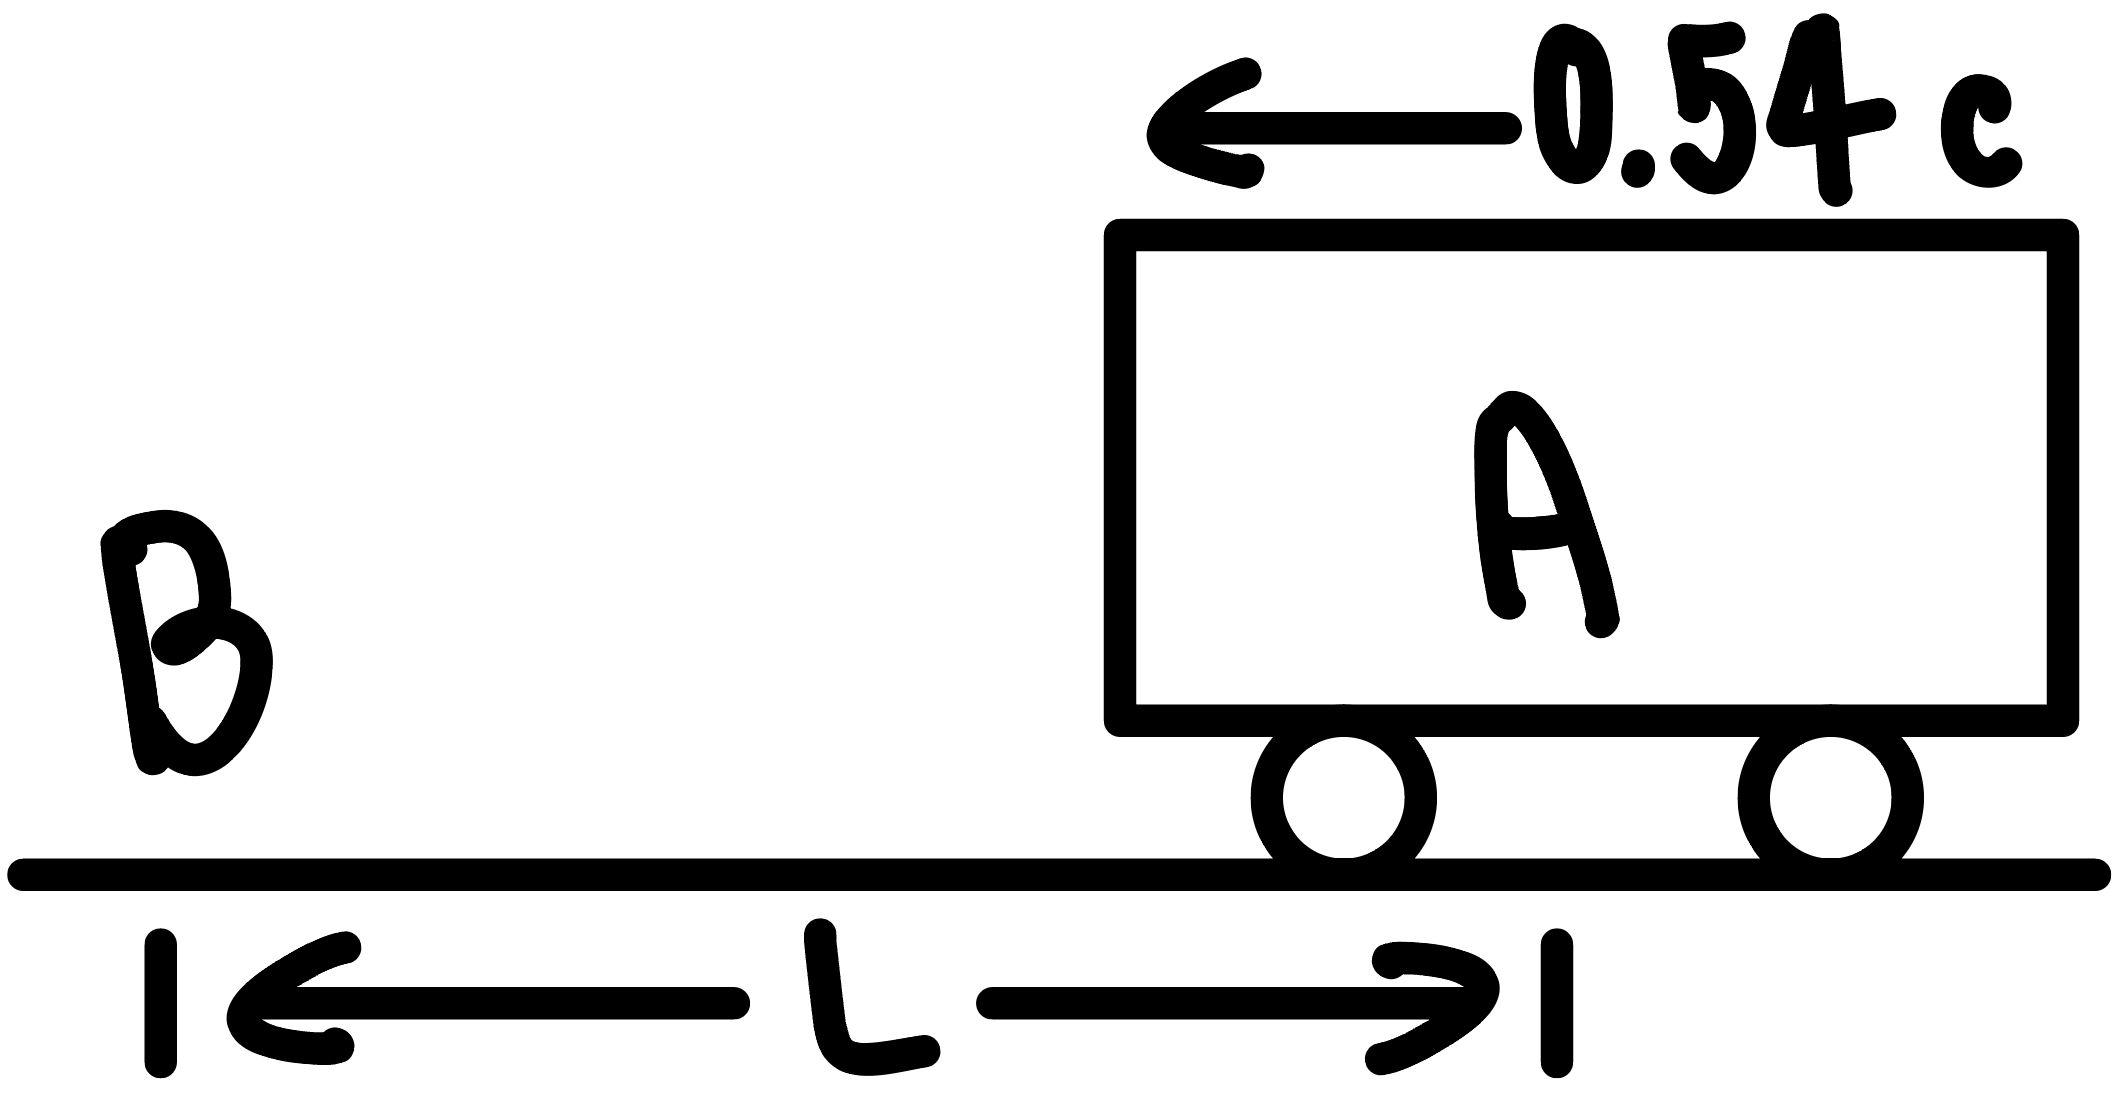
\includegraphics[width=0.325\textwidth, left]{Lorentz transformation}
\end{figure}
\noindent a) What is the coordinate of Alice in Bob's frame now?\bigskip\newline
b) What is the coordinate of Bob in Alice's frame now?\bigskip\newline
c) What is the coordinate of Alice in Bob's frame after $\D t_{B}$ time from now (time $\D t_{B}$ measured with respect to Bob)?\bigskip\newline
d) What is the coordinate of Bob in Alice's frame after $\D t_{A}$ time from now (time $\D t_{A}$ measured with respect to Alice)?\bigskip\newline
e) In Bob's frame, after how long time, Alice becomes time-like with the spacetime point $(0, 0)$?

\subsection*{3\lq (Advanced) Time dilation in general relativity (3 points)}
Alice stays on a tower with height $265\text{m}$ for $1$ hour wrt herself, while Bob stands still on the ground. Take $g=9.81\text{m}\text{s}^{-2}$.\bigskip\newline
a) How long is the time elapsed of Bob's clock for Alice's 1 hour?\bigskip\newline
b) Someone claims that if Bob moves with some speed $v$ relative to Alice, then for Alice's 1 hour, the time elapsed for Bob's clock is also 1 hour. Is this statement correct? If yes, calculate $v$.

\subsection*{4\lq Estimation of photons (2 points)}
Consider a beam of violet light with wavelength $400\text{nm}$ and total energy $30.4\text{J}$. Estimate the number of photons and total momentum of this beam of light (assuming the photons are moving in the same direction).

\subsection*{5\lq Transition of the Lithium ion (5 points)}
Consider the Lithium ion $\mathbf{Li}^{2+}$ (Lithium nuclei with one electron).\bigskip\newline
a) Use the Bohr's model (either his original model, or complemented with de Broglie's quantization) to calculate the frequency of light emitted from the transition $n_{1}\to n_{2}$ state, where $n_{1}>n_{2}$.\bigskip\newline
b) A photon is emitted due to transition involving the $n_{1}$ state. What is the highest possible frequency of the photon?\bigskip\newline
Hint: separate your answer into two cases, $n_{1}>1$ and $n_{1}=1$.

\subsection*{6\lq A finite potential barrier (10 points)}
A finite potential barrier with width $L$ is shown below. The barrier has potential energy $V_{1}$, while $V=0$ outside the barrier. The quantum particle has mass $m$ and energy $\e$.
\begin{figure}[H]
\centering
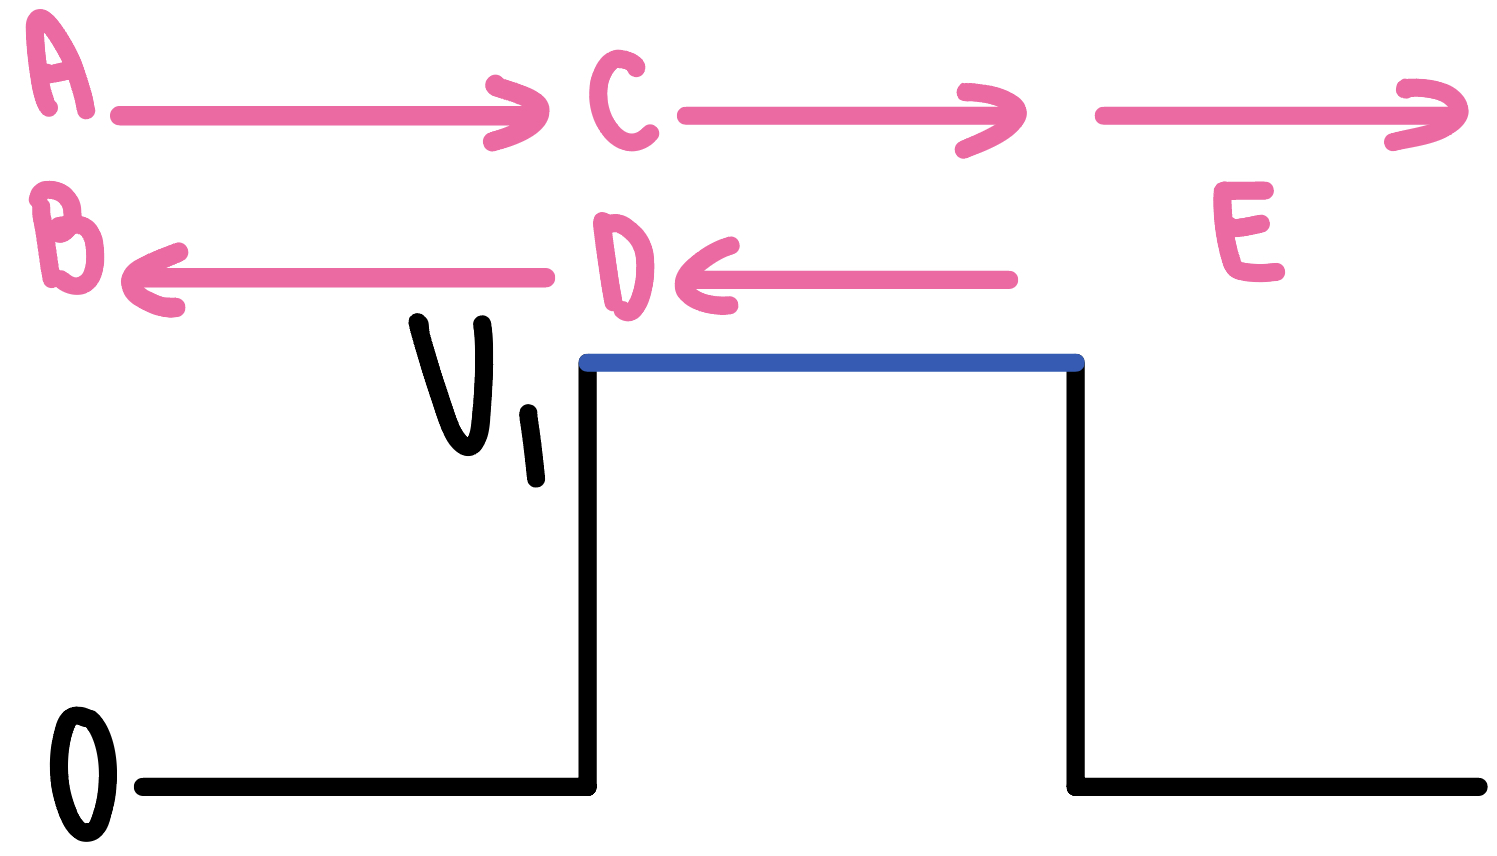
\includegraphics[width=0.4\textwidth]{A finite potential barrier}
\end{figure}

\noindent a) Derive the reflection amplitude $B$ and transmission amplitude $E$ using $A$.\bigskip\newline
Hint: prove that
\begin{align*}
\frac{B}{A}=\frac{\left(k_{0}^{2}-k_{1}^{2}\right)\left(1-e^{2ik_{1}L}\right)}{\left(k_{0}+k_{1}\right)^{2}-\left(k_{0}-k_{1}\right)^{2}e^{2ik_{1}L}}\text{ and }\frac{E}{A}=\frac{4k_{0}k_{1}e^{-i\left(k_{0}-k_{1}\right)L}}{\left(k_{0}+k_{1}\right)^{2}-\left(k_{0}-k_{1}\right)^{2}e^{2ik_{1}L}}\text{, or equivalent}
\end{align*}
b) Show that the relation between $A$, $B$ and $E$ conserves probability. The following identities may be useful.
\begin{align*}
e^{ix}+e^{-ix}&\equiv2\cos x\\
\left(k_{0}+k_{1}\right)^{4}+\left(k_{0}-k_{1}\right)^{4}&\equiv2\left(k_{0}^{2}-k_{1}^{2}\right)^{2}+16k_{0}^{2}k_{1}^{2}
\end{align*}
c) Let $\e=\frac{9}{8}V_{1}$, calculate the transmission probability of the particle. Briefly discuss the difference if the system is classical.

\subsection*{7\lq Relativistic free fall (10 points)}
The action of a free falling relativistic particle under constant gravity $g$ is
\begin{align*}
S=\int \left(\a\sqrt{1-\frac{\dot{q}^{2}}{c^{2}}}-mgq\right)\,dt
\end{align*}
a) Determine the value of $\a$ by taking the Newtonian limit $\dot{q}\ll c$.\bigskip\newline
b) Show that the system has time translation symmetry.\bigskip\newline
Hint: note that
\begin{align*}
\frac{d}{dt}\left(-\sqrt{1-\frac{\dot{q}^{2}}{c^{2}}}\d t\right)=\frac{1}{c^{2}}\left(1-\frac{\dot{q}^{2}}{c^{2}}\right)^{-\frac{1}{2}}\dot{q}\ddot{q}\d t
\end{align*}
c) Derive the conserved quantity of time translation.\bigskip\newline
d) Determine if the system has space translation symmetry $q(t)\to q(t)+\e$.

\subsection*{8\lq (Advanced) Information entropy (3 points)}
Compute the information entropy in the strings ``777", ``1416" and ``\textcolor{Lung Mun}{GLMMMNNUUUYY}". When computing probabilities for characters in a string, only consider the characters which appear in that string.

\vfill
\centerline{\bf END OF PAPER}

\newpage
\addcontentsline{toc}{section}{Solution}
\begin{center}
\textbf{\LARGE PHYS 2022 - 2022-23 Fall mock exam solution}
\rule{16.5cm}{1pt}
\end{center}
\vspace{-0.5cm}
\section*{Part I: Multiple Choice Questions (50 Points)}
1. What is the meaning of $E$ in $E=mc^{2}$, where $m$ is a constant?\\
A. Total energy\mc B. Rest energy\mc C. Kinetic energy\mc D. Potential energy\\
Comment: B. $m$ is the rest mass, and $E$ is the rest energy.\bigskip\newline
2. When I am moving in a spaceship, I do not feel my heart rate slow down compared to my watch. This is because of\\
A. the principle of relativity\mc B. the invariance of speed of light\\
C. the observer independence of physical events\mc D. the equivalence principle\\
Comment: A. An observer's proper time is defined in his own rest frame. This proper time is universal for all rest phenomena, according to the principle of relativity.\bigskip\newline
3. The ladder paradox is resolved by the fact that Alice and Bob\\
A. are not in the same reference frame\mc B. have different length of ruler\\
C. have different sense of ``same time"\mc D. have different time elapsing speed\\
Comment: C. The relativity of simultaneity and flexibility of time ordering for events with space-like separation resolves the ladder paradox.\bigskip\newline
4. Alice and Bob are inertial observers with a relative speed. Which statement is correct?\\
A. According to what Alice sees (light to her eyes), Bob slows down\\
B. According to Alice's frame time, Bob slows down\\
C. According to what Alice sees (light to her eyes), Bob speeds up\\
D. According to Alice's frame time, Bob speeds up\\
Comment: B. Time dilation is for measurement time, not visual time.\bigskip\newline
5. For $v_{1}=0.5c$ and $v_{2}=c$ in the same direction, what is the velocity addition of $v_{1}$ and $v_{2}$ in special relativity?\\
A. $0.5c$\mc B. $0.75c$\mc C. $c$\mc D. $1.5c$\\
Comment: C. According to the invariance of light speed, the addition of any velocity to the light speed $c$ gives $c$.\bigskip\newline
6. Which of the following is NOT an expression of relativistic momentum?\\
A. $\c m\frac{dx}{dt}$\mc B. $m\frac{dx}{d\t}$\mc C. $mc\tanh^{-1}\left(\frac{v}{c}\right)$\mc D. $\sqrt{\frac{E^{2}}{c^{2}}-m^{2}c^{2}}$\\
Comment: C. It is easy to check that the other three options are expressions of relativistic momentum.\bigskip\newline
7. Alice is moving from right to left with respect to Bob. Consider two space-like events $P$ and $Q$ with $x_{P}>x_{Q}$ in Alice's space coordinate. Which of the following is impossible?\\
A. Both Alice and Bob consider $P$ earlier than $Q$\\
B. Both Alice and Bob consider $P$ later than $Q$\\
C. Alice considers $P$ earlier than $Q$; Bob considers $P$ later than $Q$\\
D. Alice considers $P$ later than $Q$; Bob considers $P$ earlier than $Q$\\
Comment: C. Try to draw a spacetime diagram.\bigskip\newline
8. If two events have causal relation, these two events are\\
A. space-like\mc B. time-like\mc C. space-like or light-like\mc D. time-like or light-like\\
Comment: D. Space-like separation requires superluminal propagation to establish causal relation, which is forbidden in relativity.\bigskip\newline
9. (Advanced) In general relativity, a person standing in front of you appears slightly taller because the Earth gravity has the effect of\\
A. frame dragging\mc B. time dilation\mc C. length contraction\mc D. light bending\\
Comment: D. Earth's gravity bends the light downwards, causing the image to appear taller than the original object.\bigskip\newline
10. (Advanced) If gravity is not uniform, which of the following is correct?\\
A. We can apply the equivalence principle to cancel gravity everywhere\\
B. We can apply the equivalence principle to cancel gravity locally at a point\\
C. There will not be time dilation in non-uniform gravity\\
D. General relativity cannot deal with non-uniform gravity\\
Comment: B. For non-uniform gravity, equivalence principle holds for infinitesimal inertial frames, i.e. locally at a small region near a point.\bigskip\newline
11. (Advanced) Alice is falling into a large black hole from outside the horizon, and Bob watches the event very far away outside the horizon. Which of the following is NOT correct?\\
A. Alice reaches the black hole singularity at finite time\\
B. Alice finds nothing special when crossing the black hole horizon\\
C. Bob finds Alice being slow when she is falling towards the black hole\\
D. Bob can see that Alice reaches the black hole singularity\\
Comment: D. According to general relativity, information inside the event horizon of the black hole cannot get out.\bigskip\newline
12. (Advanced) Now we can observe gravitational waves from merging events of two black holes. Which of the following is NOT correct?\\
A. If the masses of the two initial black holes are $36$ and $29$ solar mass respectively, then the final merged black hole should have mass equal to $65$ solar mass\\
B. The observed gravitational waves has to be emitted outside the black hole's horizon\\
C. In the vacuum, gravitational waves propagate at the speed of light\\
D. Building more than two detectors can improve the precision of locating the source of gravitational
waves in the sky\\
Comment: A. Due to the energy carried away by the emitted gravitational waves, the mass of the final black hole is strictly smaller than the mass of the sum.\bigskip\newline
13. (Advanced) The night sky is dark, mainly because of\\
A. the finite age of the universe\mc B. the finite size of the entire universe\\
C. the finite energy density of the universe\mc D. the finite lifetime of stars\\
Comment: A. The speed of light is finite, and light travels a finite distance within the finite age of the universe, so only finitely many stars can be observed from Earth. The density of stars in the finite observable volume is sufficiently low, such that any line of sight from Earth is unlikely to reach a star.\bigskip\newline
14. The quantum wave function is a wave of\\
A. probability density\mc B. probability amplitude\\
C. mechanical oscillation\mc D. mechanical oscillation amplitude\\
Comment: B. The quantum wave function $\psi$ is a wave of probability amplitude, while the probability density is $\left|\psi\right|^{2}$.\bigskip\newline
15. Which is NOT a property of a photon?\\
A. It has energy and momentum\mc B. Its wavelength can vary continuously\\
C. Its amplitude can vary continuously\mc D. It can interfere with itself\\
Comment: C. The wavelength of a photon can vary continuously, e.g. in gravitational redshift. However, its amplitude cannot.\bigskip\newline
16. Which is WRONG for superposition of quantum states?\\
A. Probability distribution of the particle can be added from component states\\
B. Quantum superposition is linear\\
C. The resulting state may have indefinite momentum\\
D. The resulting state may have indefinite energy\\
Comment: A. Generally, $\left|\psi_{1}+\psi_{2}\right|^{2}\neq\left|\psi_{1}\right|^{2}+\left|\psi_{2}\right|^{2}$.\bigskip\newline
17. Which is WRONG for quantum measurements?\\
A. A measurement can be modelled as an operator\\
B. The wave function may collapse because of the measurement\\
C. Results of multiple measurements may depend on the order of these measurements\\
D. The measured outcome may be complex-valued instead of a real number\\
Comment: D. The outcome of a quantum measurement must be a real number.\bigskip\newline
18. Which of the following about bosons and fermions is WRONG?\\
A. Bosons represent force and fermions represent matter for fundamental particles\\
B. The wave function of multiple Bosonic identical particles is symmetric\\
C. The wave function of multiple Fermion identical particles is anti-symmetric\\
D. There can only be one fermion on each energy level of the system\\
Comment: D. Pauli's exclusion principle states that two or more identical fermions cannot occupy the same quantum state, but not energy level.\bigskip\newline
19. For an infinite potential well, which of the following would break?\\
A. The wave function must be continuous\\
B. The first derivative of the wave function must be continuous\\
C. The probability amplitude interpretation of the wave function\\
D. The existence of bound states\\
Comment: B. The first derivative of the wave function is discontinuous at the boundary, where the potential is infinite.\bigskip\newline
20. Which of the following experiment indicates that the world is made of atoms?\\
A. Dalton's multiple proportions\mc B. Newton's decomposition of white light\\
C. Rutherford's $\a$-particle scattering\mc D. Young's double slit experiment\\
Comment: A. Dalton's experiment of multiple proportions shows that elements combine in simple ratios to form compounds, which is an evidence to the atomic theory.\bigskip\newline
21. For which of the below elements (in their ground states), the outermost electron is not in the $\text{s}$ orbital?\\
A. Hydrogen ($\mathbf{H}$)\mc B. Helium ($\mathbf{He}$)\\
C. Carbon ($\mathbf{C}$)\mc D. Potassium ($\mathbf{K}$)\\
Comment: C. The electronic configuration of $\mathbf{C}$ is $1\text{s}^{2}2\text{s}^{2}2\text{p}^{2}$.\bigskip\newline
22. (Advanced) What is the result of $\s_{1}\ket{\odot}$?\\
A. $i\ket{\odot}$\mc B. $-i\ket{\otimes}$\mc C. $i\ket{\rightarrow}$\mc D. $-i\ket{\leftarrow}$\\
Comment: B. By direct computation,
\begin{align*}
\s_{1}\ket{\odot}&=
\begin{pmatrix}
0&1\\
1&0
\end{pmatrix}
\frac{1}{\sqrt{2}}
\begin{pmatrix}
1\\
-i
\end{pmatrix}\\
&=\frac{1}{\sqrt{2}}
\begin{pmatrix}
-i\\
1
\end{pmatrix}\\
&=-i\ket{\otimes}
\end{align*}
23. (Advanced) About the EPR paradox, which of the following is WRONG?\\
A. To measure each of the particle in the EPR pair individually, random result is obtained\\
B. Measurements on the pair are correlated\\
C. The correlation of the measurement is not limited by the speed of light\\
D. The nature of EPR pairs can be mimicked by a local hidden variable theory\\
Comment: D. EPR paradox violates classical logic, therefore the nature of EPR pairs cannot be mimicked by a local hidden theory.\bigskip\newline
24. (Advanced) What protects the second law of thermodynamics in the Maxwell's demon thought experiment?\\
A. Effort to lift the gate\\
B. Quantum measurement of the particle speed\\
C. Interaction between the gas particles\\
D. Overwritten information in the demon's memory\\
Comment: D. Due to the overwritten information in the demon's memory, either the entropy of his brain increases, or heat is generated in his body.\bigskip\newline
25. (Advanced) What is the information entropy of ``AAIIMST"?\\
A. $-\frac{4}{7}+\log_{2}7$\mc B. $-\frac{4}{7}+\log_{2}6$\mc C. $-\frac{8}{7}+\frac{11}{7}\log_{2}7$\mc D. $-\frac{8}{7}+\frac{11}{7}\log_{2}6$\\
Comment: A. $P(``\text{A}")=P(``\text{I}")=\frac{2}{7}$ and $P(``\text{M}")=P(``\text{S}")=P(``\text{T}")=\frac{1}{7}$, so
\begin{align*}
H(``\text{AAIIMST}")&=2\times\frac{2}{7}\log_{2}\frac{7}{2}+3\times\frac{1}{7}\log_{2}7\\
&=-\frac{4}{7}+\log_{2}7
\end{align*}

\begin{solbox}
BACBC\mc CCDDB\mc DAABC\mc ADDBA\mc CBDDA
\end{solbox}

\section*{Part II: Long Questions (50 points)}
\subsection*{1\lq Collision of two masses (5 points)}
A particle A of rest mass $m_{A}$ collides head-on with another particle B of rest mass $m_{B}$ in $1$ space direction. Before the collision, B has energy $Q$. After the collision, B still has energy $Q$, but it is moving in the opposite direction. Express the quantities below using $m_{A}$, $m_{B}$, c and Q.\bigskip\newline
a) What is the relativistic momentum of $B$ before and after the collision?\bigskip\newline
b) What is the relativistic momentum and energy of $A$ before and after the collision?\bigskip\newline
c) What is the speed of $A$ before and after the collision?

\begin{solbox}
a) (1 point)\\
Suppose A is initially moving towards the right and B towards the left.
\begin{align*}
E_{B}&=E_{B}'=m_{B}^{2}c^{4}+\left|p_{B}\right|^{2}c^{2}=Q^{2}\\
p_{B}&=\mp\sqrt{\frac{Q^{2}-m_{B}^{2}c^{4}}{c^{2}}}
\end{align*}
where ``$-$'' sign is before collision and ``$+$'' sign is after collision (the overall $\mp$ sign depends on the choice of coordinates, the answer is correct as long as there is a relative sign difference).\bigskip\newline
b) (2 points)\\
By energy conservation,
\begin{align*}
E_{A}+E_{B}&=E_{A}'+E_{B}'
\end{align*}
Since $E_{B}=E_{B}'=Q$, we have $E_{A}=E_{A}'$, which implies $p_{A}=p_{A}'$.\bigskip\newline
By momentum conservation,
\begin{align*}
p_{A}+p_{B}&=p_{A}'+p_{B}'\\
p_{A}-p_{A}'&=p_{B}'-p_{B}=2\sqrt{\frac{Q^{2}-m_{B}^{2}c^{4}}{c^{2}}}\\
2\left|p_{A}\right|&=2\sqrt{\frac{Q^{2}-m_{B}^{2}c^{4}}{c^{2}}}\\
p_{A}&=\pm\sqrt{\frac{Q^{2}-m_{B}^{2}c^{4}}{c^{2}}}
\end{align*}
where ``$+$" sign is before collision and ``$-$'' sign is after collision.\bigskip\newline
The energy of A can be obtained from the dispersion relation,
\begin{align*}
E_{A}&=\sqrt{p_{A}^{2}c^{2}+m_{A}^2 c^4}\\
&=\sqrt{Q^2+\left(m_{A}^{2}-m_{B}^{2}\right)c^4}
\end{align*}
It is the same before and after collision.\bigskip\newline
c) (2 points)\\
The expression of relativistic energy is $E_{A}=\c m_{A}c^2$. Using the result in (b),
\begin{align*}
\sqrt{Q^2+\left(m_{A}^{2}-m_{B}^{2}\right)c^4}&=\c m_{A}c^2\\
\frac{1}{\sqrt{1-\frac{v_{A}^2}{c^2}}}&=\frac{\sqrt{Q^2+\left(m_{A}^{2}-m_{B}^{2}\right)c^4}}{m_{A}c^2}
\end{align*}
After solving,
\begin{align*}
v_{A}=\pm\sqrt{\frac{Q^{2}-m_{B}^{2}c^{4}}{Q^{2}/c^{2}+\left(m_{A}^{2}-m_{B}^{2}\right)c^{2}}}
\end{align*}
where ``$+$" sign is before collision and ``$-$" sign is after collision.
\end{solbox}

\subsection*{2\lq Lorentz transformation (12 points)}
Alice is moving with speed $0.54c$ towards Bob. Now, the distance between Alice and Bob is $L$ in Bob's frame. Let Bob's spacetime coordinate in his own frame be $(t_{B}, x_{B})=(0, 0)$, and Alice's spacetime coordinate in her own frame be $(t_{A}, x_{A})=(0, 0)$.
\begin{figure}[H]
\centering
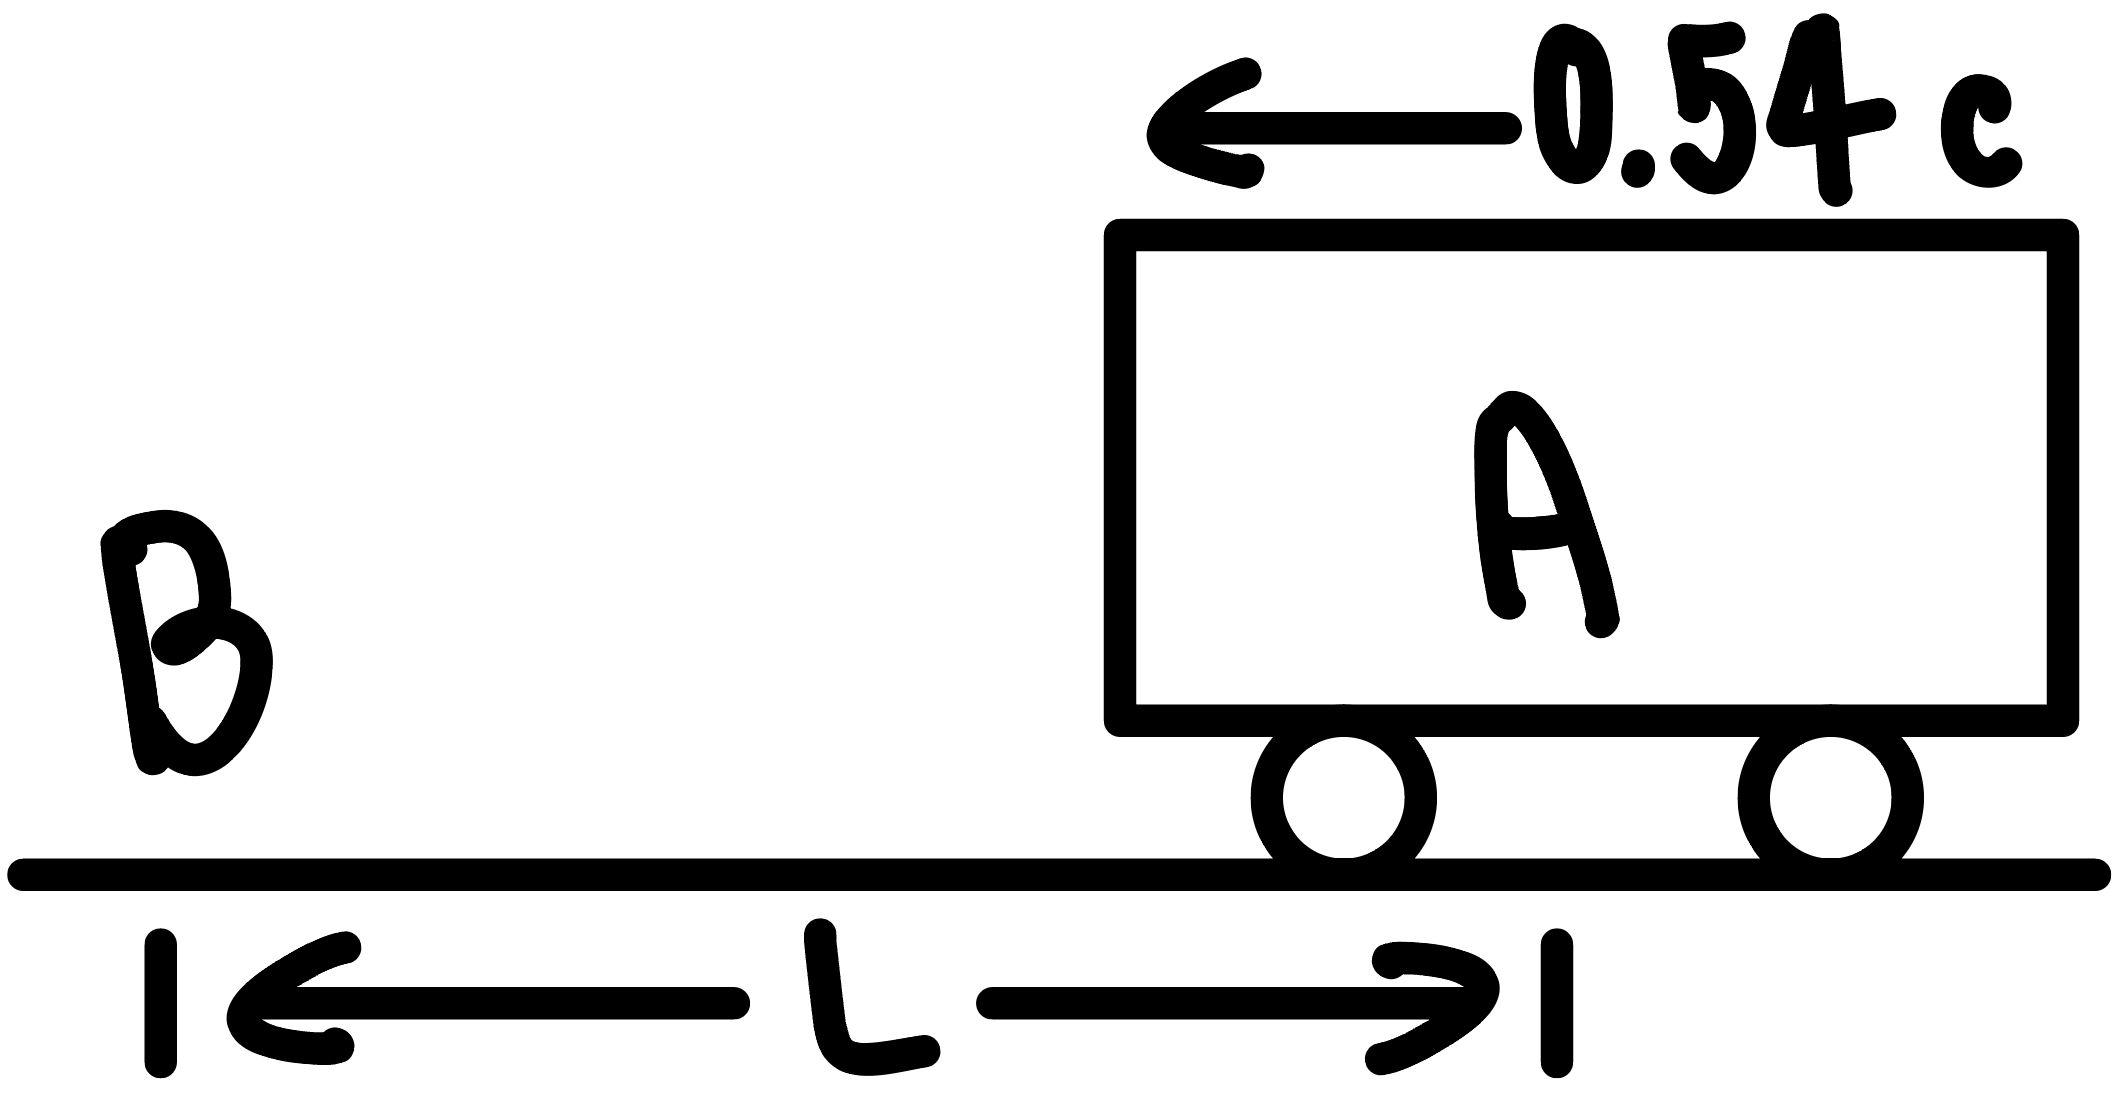
\includegraphics[width=0.325\textwidth, left]{Lorentz transformation}
\end{figure}
\noindent a) What is the coordinate of Alice in Bob's frame now?\bigskip\newline
b) What is the coordinate of Bob in Alice's frame now?\bigskip\newline
c) What is the coordinate of Alice in Bob's frame after $\D t_{B}$ time from now (time $\D t_{B}$ measured with respect to Bob)?\bigskip\newline
d) What is the coordinate of Bob in Alice's frame after $\D t_{A}$ time from now (time $\D t_{A}$ measured with respect to Alice)?\bigskip\newline
e) In Bob's frame, after how long time, Alice becomes time-like wrt the spacetime point $(0, 0)$?

\begin{solbox}
a) (2 points)\\
The coordinate of Alice in Bob's frame is $\left(t_{B, A0}, x_{B, A0}\right)=(0, L)$.\bigskip\newline
There are two ways to define ``now", and each definition corresponds to a set of consistent answers for (b) to (e).
\subsubsection{Define ``now" as in Alice's frame}
b) (2 points)\\
We first define ``now" as in Alice's frame, and the time coordinate of Bob in Alice's frame now is $t_{A, B0}=0$. Wrt Alice, the ground is moving relative to her, her distance to Bob is thus contracted to $L'=\frac{L}{\c}$. The coordinate of Bob in Alice's frame is
\begin{align*}
\left(t_{A, B0}, x_{A, B0}\right)&=\left(0, -\frac{L}{\c}\right)\\
&=\left(0, -\frac{L}{1.19}\right)
\end{align*}
c) (3 points)\\
The coordinate of Alice in Bob's frame after $\D t_{B}$ is $\left(t_{B, A1}, x_{B, A1}\right)$, where
\begin{align*}
t_{B, A1}&=t_{B, A0}+\D t_{B}=\D t_{B}\\
x_{B, A1}&=t_{B, A1}+v\D t_{B}=L-0.54c\D t_{B}
\end{align*}
d) (3 points)\\
The coordinate of Bob in Alice's frame after $\D t_{A}$ is $\left(t_{A, B1}, x_{A, B1}\right)$, where
\begin{align*}
t_{A, B1}&=t_{A, B0}+\D t_{A}=\D t_{A}\\
x_{A, B1}&=x_{A, B0}-v\D t_{A}=-\frac{L}{1.19}+0.54c\D t_{A}
\end{align*}
e) (2 points)\\
Alice becomes time-like wrt the spacetime point $\left(t_{B, B0}, x_{B, B0}\right)=(0, 0)$ when the spacetime interval crosses zero.
\begin{align*}
-c^{2}\D t^{2}+\D x^{2}&=0\\
-c^{2}\left(t_{B, A2}-t_{B, B0}\right)^{2}+\left(x_{B, A2}-x_{B, B0}\right)^{2}&=0\\
x_{B, A2}&=x_{B, A0}+v\left(t_{B, A2}-t_{B, A0}\right)\\
&=L+vt_{B, A2}\\
\implies -c^{2}t_{B, A2}^{2}+\left(L+vt_{B, A2}\right)^{2}&=0
\end{align*}
After solving, we obtain
\begin{align*}
t_{B, A2}=\frac{L}{c-v}=\frac{L}{1.54c}
\end{align*}

\subsubsection{Define ``now" as in Bob's frame}
b) (2 points)\\
We can also define ``now" as in Bob's frame. Applying Lorentz transformation,
\begin{align*}
t_{B}&=\c\left(t_{A}+\frac{v}{c^{2}}x_{A}\right)\implies t_{A}+\frac{v}{c^{2}}x_{A}=\frac{1}{\c}t_{B}\\
x_{B}&=\c\left(x_{A}+vt_{A}\right)+L\implies x_{A}+vt_{A}=\frac{1}{\c}\left(x_{B}-L\right)
\end{align*}
After solving these two equations,
\begin{align*}
t_{A}&=\c\left(t_{B}-\frac{v}{c^{2}}x_{A}+\frac{vL}{c^{2}}\right)\\
x_{A}&=\c\left(x_{B}-vt_{B}-L\right)
\end{align*}
Put $\left(t_{B, B0}, x_{B, B0}\right)=(0, 0)$, the coordinate of Bob in Alice's frame is
\begin{align*}
\left(t_{A, B0}, x_{A, B0}\right)&=\left(-\frac{1.19L}{c}, -0.642L\right)
\end{align*}
c) (3 points)\\
The coordinate of Alice in Bob's frame after $\D t_{B}$ is $\left(t_{B, A1}, x_{B, A1}\right)$, where
\begin{align*}
t_{B, A1}&=t_{B, A0}+\D t_{B}=\D t_{B}\\
x_{B, A1}&=t_{B, A1}+v\D t_{B}=L-0.54c\D t_{B}
\end{align*}
d) (3 points)\\
The coordinate of Bob in Alice's frame after $\D t_{A}$ is $\left(t_{A, B1}, x_{A, B1}\right)$, where
\begin{align*}
t_{A, B1}&=t_{A, B0}+\D t_{A}=-\frac{1.19L}{c}+\D t_{A}\\
x_{A, B1}&=x_{A, B0}-v\D t_{A}=-0.642L+0.54c\D t_{A}
\end{align*}
e) (2 points)
\begin{align*}
t_{B, A2}=\frac{L}{c-v}=\frac{L}{1.54c}
\end{align*}
\end{solbox}

\subsection*{3\lq (Advanced) Time dilation in general relativity (3 points)}
Alice stays on a tower with height $265\text{m}$ for $1$ hour wrt herself, while Bob stands still on the ground. Take $g=9.81\text{m}\text{s}^{-2}$.\bigskip\newline
a) How long is the time elapsed of Bob's clock for Alice's 1 hour?\bigskip\newline
b) Someone claims that if Bob moves with some speed $v$ relative to Alice, then for Alice's 1 hour, the time elapsed for Bob's clock is also 1 hour. Is this statement correct? If yes, calculate $v$.

\begin{solbox}
a) (1 point)
\begin{align*}
\D t_{B}&=\left(1+\frac{\phi_{B}-\phi_{A}}{c^{2}}\right)\\
&=\left(1-\frac{gh}{c^{2}}\right)\D t_{A}\\
&=\left(1-2.89\times10^{-14}\right)\times 1\text{hr}
\end{align*}
b) (2 points)\\
There is an extra time dilation factor $\c$,
\begin{align*}
\D t_{B}&=\c\left(1-\frac{gh}{c^{2}}\right)\D t_{A}\\
&=\frac{1}{\sqrt{1-\frac{v^{2}}{c^{2}}}}\left(1-\frac{gh}{c^{2}}\right)\D t_{A}
\end{align*}
We want to find $v$ such that $\D t_{B}=\D t_{A}=1\text{hr}$, so
\begin{align*}
\c\left(1-\frac{gh}{c^{2}}\right)&=1\\
\frac{1}{\sqrt{1-\frac{v^{2}}{c^{2}}}}\left(1-\frac{gh}{c^{2}}\right)&=1
\end{align*}
After solving,
\begin{align*}
v&=\sqrt{2gh-\frac{g^{2}h^{2}}{c^{2}}}\\
&=72.1\text{m}\text{s}^{-1}
\end{align*}
Using Taylor's expansion to get $v=\sqrt{2gh}=72.1\text{m}\text{s}^{-1}$ is also allowed.
\end{solbox}

\subsection*{4\lq Estimation of photons (2 points)}
Consider a beam of violet light with wavelength $400\text{nm}$ and total energy $30.4\text{J}$. Estimate the number of photons and total momentum of this beam of light (assuming the photons are moving in the same direction).

\begin{solbox}
Let $N$ be the total number of photons.
\begin{align*}
N\cdot\frac{hc}{\l}&=E\\
N&=\frac{E\l}{hc}\\
&=6.12\times10^{19}
\end{align*}
For particles with zero rest mass, we have $E=pc$, so
\begin{align*}
p&=\frac{E}{c}\\
&=1.01\times10^{-7}\text{kg}\text{m}\text{s}^{-1}
\end{align*}
\end{solbox}

\subsection*{5\lq Transition of the Lithium ion (5 points)}
Consider the Lithium ion $\mathbf{Li}^{2+}$ (Lithium nuclei with one electron).\bigskip\newline
a) Use the Bohr's model (either his original model, or complemented with de Broglie's quantization) to calculate the frequency of light emitted from the transition $n_{1}\to n_{2}$ state, where $n_{1}>n_{2}$.\bigskip\newline
b) A photon is emitted due to transition involving the $n_{1}$ state. What is the highest possible frequency of the photon?\bigskip\newline
Hint: separate your answer into two cases, $n_{1}>1$ and $n_{1}=1$.

\begin{solbox}
a) (3 points)\\
The centripetal force on the electron is provided by the Coulomb force,
\begin{align*}
\frac{mv^{2}}{r}&=\frac{1}{4\pi\e_{0}}\frac{Ze^{2}}{r^{2}}\\
\implies mv^{2}r&=\frac{Ze^{2}}{4\pi\e_{0}}
\end{align*}
The potential energy of the electron is given by $V(r)=-\frac{1}{4\pi\e_{0}}\frac{Ze^{2}}{r}$, so its total energy is
\begin{align*}
E&=\frac{1}{2}mv^{2}+V(r)\\
&=-\frac{1}{2}mv^{2}\\
&=-\frac{1}{2}\cdot\frac{Ze^{2}}{4\pi\e_{0}r}
\end{align*}
Using de Broglie's approach,
\begin{align*}
2\pi r&=n\l\\
\l&=\frac{h}{mv}
\end{align*}
Combining these two equations,
\begin{align*}
mvr=\frac{nh}{2\pi}
\end{align*}
The speed $v$ of the electron is thus
\begin{align*}
v=\frac{mv^{2}r}{mvr}&=\frac{Ze^{2}}{4\pi\e_{0}}\cdot \frac{2\pi}{nh}\\
&=\frac{Ze^{2}}{2\e_{0}nh}
\end{align*}
Substitute the result to the total energy,
\begin{align*}
E_{n}&=-\frac{1}{2}mv^{2}\\
&=-\frac{1}{2}m\cdot \frac{Z^{2}e^{4}}{4\e_{0}^{2}n^{2}h^{2}}\\
&=-\frac{Z^{2}me^{4}}{8\e_{0}^{2}n^{2}h^{2}}
\end{align*}
When the electron transits from the $n_{1}$ state to the $n_{2}$ state, the difference in energy is
\begin{align*}
\D E=-\frac{Z^{2}me^{4}}{8\e_{0}^{2}h^{2}}\left(\frac{1}{n_{1}^{2}}-\frac{1}{n_{2}^{2}}\right)
\end{align*}
The Lithium ion has $Z=3$, so the frequency of light emitted is
\begin{align*}
\nu&=-\frac{Z^{2}me^{4}}{8\e_{0}^{2}h^{3}}\left(\frac{1}{n_{1}^{2}}-\frac{1}{n_{2}^{2}}\right)\\
&=-\frac{9me^{4}}{8\e_{0}^{2}h^{3}}\left(\frac{1}{n_{1}^{2}}-\frac{1}{n_{2}^{2}}\right)
\end{align*}
b) (2 points)\\
For $n_{1}>1$, $n_{1}$ can be the initial or the final state.
\subsubsection{$n_{1}$ as the initial state}
If $n_{1}$ is the initial state, it can transit to another state $n_{2}<n_{1}$.
\begin{align*}
\nu&=-\frac{9me^{4}}{8\e_{0}^{2}h^{3}}\left(\frac{1}{n_{1}^{2}}-\frac{1}{n_{2}^{2}}\right)\\
&=\frac{9me^{4}}{8\e_{0}^{2}h^{3}}\left(\frac{1}{n_{2}^{2}}-\frac{1}{n_{1}^{2}}\right)\\
&\leq \frac{9me^{4}}{8\e_{0}^{2}h^{3}}\left(1-\frac{1}{n_{1}^{2}}\right)
\end{align*}

\subsubsection{$n_{1}$ as the final state}
If $n_{1}$ is the final state, another state $n_{2}>n_{1}$ can transit to it.
\begin{align*}
\nu&=-\frac{9me^{4}}{8\e_{0}^{2}h^{3}}\left(\frac{1}{n_{2}^{2}}-\frac{1}{n_{1}^{2}}\right)\\
&=\frac{9me^{4}}{8\e_{0}^{2}h^{3}}\left(\frac{1}{n_{1}^{2}}-\frac{1}{n_{2}^{2}}\right)\\
&\leq \frac{9me^{4}}{8\e_{0}^{2}h^{3}}\cdot\frac{1}{n_{1}^{2}}
\end{align*}
We notice that
\begin{align*}
n_{1}>\sqrt{2}\implies 1-\frac{1}{n_{1}^{2}}>\frac{1}{n_{1}^{2}}
\end{align*}
Thus, for $n_{1}>1$, where $n_{1}\in\N$, we have
\begin{align*}
\nu_{\text{max}}=\frac{9me^{4}}{8\e_{0}^{2}h^{3}}\left(1-\frac{1}{n_{1}^{2}}\right)
\end{align*}
For $n_{1}=1$, $n_{1}$ must be the final state, so
\begin{align*}
\nu&=-\frac{9me^{4}}{8\e_{0}^{2}h^{3}}\left(\frac{1}{n_{2}^{2}}-\frac{1}{n_{1}^{2}}\right)\\
&=\frac{9me^{4}}{8\e_{0}^{2}h^{3}}\left(\frac{1}{n_{1}^{2}}-\frac{1}{n_{2}^{2}}\right)\\
&\leq \frac{9me^{4}}{8\e_{0}^{2}h^{3}}
\end{align*}
When $n_{1}=1$,
\begin{align*}
\nu_{\text{max}}=\frac{9me^{4}}{8\e_{0}^{2}h^{3}}
\end{align*}
\end{solbox}

\subsection*{6\lq A finite potential barrier (10 points)}
A finite potential barrier with width $L$ is shown below. The barrier has potential energy $V_{1}$, while $V=0$ outside the barrier. The quantum particle has mass $m$ and energy $\e$.
\begin{figure}[H]
\centering
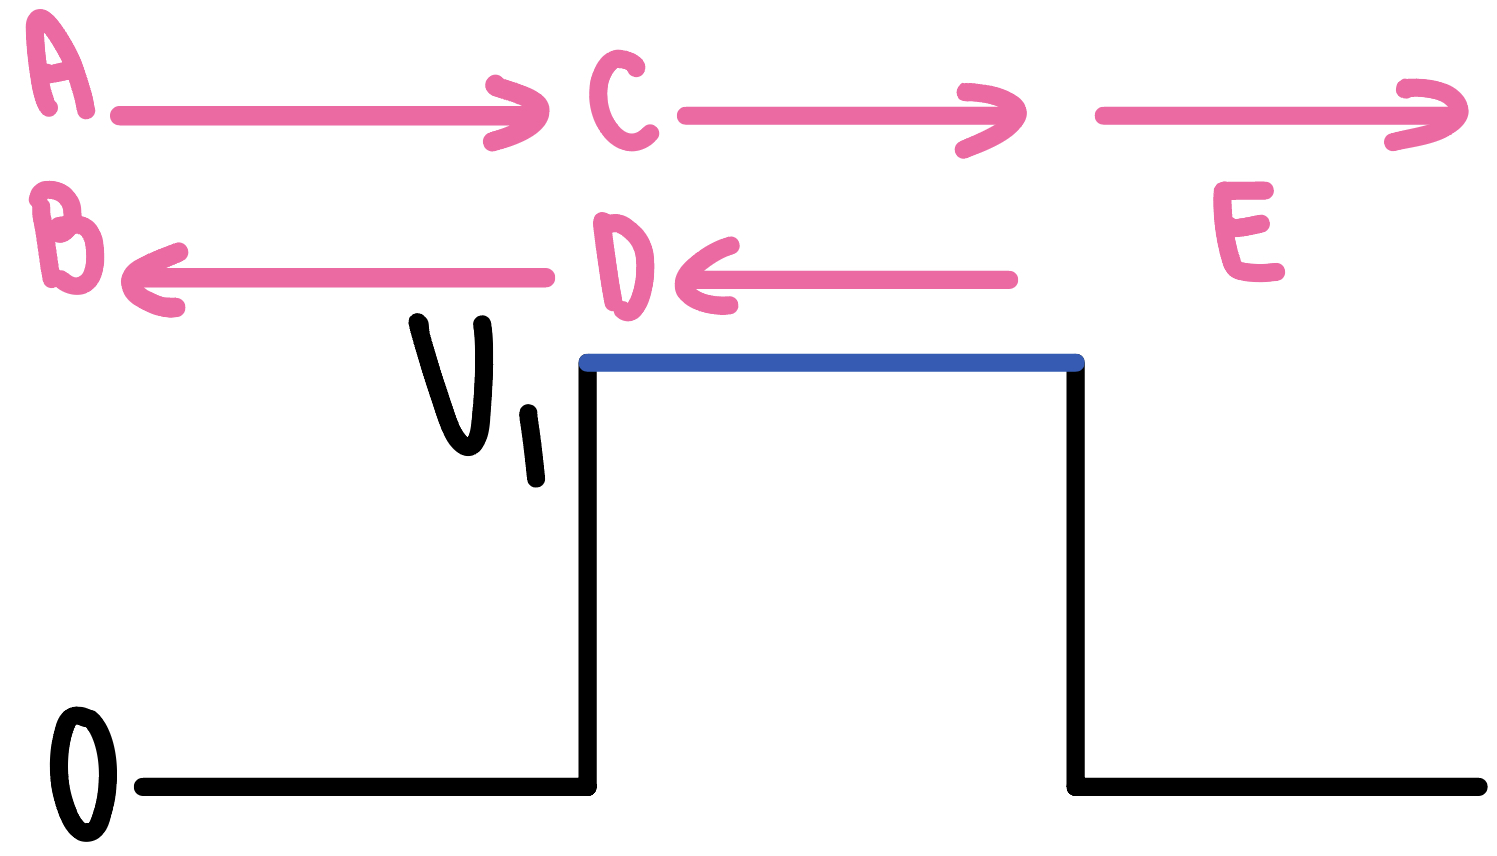
\includegraphics[width=0.4\textwidth]{A finite potential barrier}
\end{figure}

\noindent a) Derive the reflection amplitude $B$ and transmission amplitude $E$ using $A$.\bigskip\newline
Hint: prove that
\begin{align*}
\frac{B}{A}=\frac{\left(k_{0}^{2}-k_{1}^{2}\right)\left(1-e^{2ik_{1}L}\right)}{\left(k_{0}+k_{1}\right)^{2}-\left(k_{0}-k_{1}\right)^{2}e^{2ik_{1}L}}\text{ and }\frac{E}{A}=\frac{4k_{0}k_{1}e^{-i\left(k_{0}-k_{1}\right)L}}{\left(k_{0}+k_{1}\right)^{2}-\left(k_{0}-k_{1}\right)^{2}e^{2ik_{1}L}}\text{, or equivalent}
\end{align*}
b) Show that the relation between $A$, $B$ and $E$ conserves probability. The following identities may be useful.
\begin{align*}
e^{ix}+e^{-ix}&\equiv2\cos x\\
\left(k_{0}+k_{1}\right)^{4}+\left(k_{0}-k_{1}\right)^{4}&\equiv2\left(k_{0}^{2}-k_{1}^{2}\right)^{2}+16k_{0}^{2}k_{1}^{2}
\end{align*}
c) Let $\e=\frac{9}{8}V_{1}$, calculate the transmission probability of the particle. Briefly discuss the difference if the system is classical.

\begin{solbox}
a) (5 points)\\
The potential function is
\begin{align*}
V(x)=
\begin{cases}
V_{1}\text{ if }0<x<L\\
0\text{ if }x<0\text{ or }x>L
\end{cases}
\end{align*}
We start with the time-independent Schr\"{o}dinger equation,
\begin{align*}
\left[-\frac{\hbar^{2}}{2m}\frac{d^{2}}{dx^{2}}+V(x)\right]\psi(x)=\e\psi(x)
\end{align*}
After rearrangement,
\begin{align*}
\frac{d^{2}}{dx^{2}}\psi(x)+k^{2}(x)\psi(x)=0
\end{align*}
where $k(x)\equiv\frac{\sqrt{2m(\e-V(x))}}{\hbar}$.\bigskip\newline
The solution of the wave function is
\begin{align*}
\psi(x)=
\begin{cases}
Ae^{ik_{0}x}+Be^{-ik_{0}x}\text{ if }x<0\\
Ce^{ik_{1}x}+De^{-ik_{1}x}\text{ if }0<x<L\\
Ee^{ik_{0}x}\text{ if }x>L
\end{cases}
\end{align*}
where $k_{0}\equiv\frac{\sqrt{2m\e}}{\hbar}$ and $k_{1}\equiv\frac{\sqrt{2m(\e-V_{1})}}{\hbar}$.\bigskip\newline
By the continuity conditions at $x=0$,
\begin{align*}
\psi_{-}(0)&=\psi_{+}(0)\implies A+B=C+D\\
\psi'_{-}(0)&=\psi'_{+}(0)\implies k_{0}(A-B)=k_{1}(C-D)
\end{align*}
Similarly, by the continuity conditions at $x=L$,
\begin{align*}
\psi_{-}(L)&=\psi_{+}(L)\implies Ce^{ik_{1}L}+De^{-ik_{1}L}=Ee^{ik_{0}L}\\
\psi'_{-}(L)&=\psi'_{+}(L)\implies k_{1}\left(Ce^{ik_{1}L}-De^{-ik_{1}L}\right)=k_{0}E^{ik_{0}L}
\end{align*}
Solving the first two equations, we get
\begin{align*}
A&=\frac{k_{0}+k_{1}}{2k_{0}}C+\frac{k_{0}-k_{1}}{2k_{0}}D\\
B&=\frac{k_{0}-k_{1}}{2k_{0}}C+\frac{k_{0}+k_{1}}{2k_{0}}D\\
\implies \frac{B}{A}&=\frac{(k_{0}-k_{1})C+(k_{0}+k_{1})D}{(k_{0}+k_{1})C+(k_{0}-k_{1})D}
\end{align*}
Solving the last two equations, we get
\begin{align*}
Ce^{ik_{1}L}&=\frac{k_{0}+k_{1}}{2k_{1}}Ee^{ik_{0}L}\\
De^{-ik_{1}L}&=\frac{k_{1}-k_{0}}{2k_{1}}Ee^{ik_{0}L}\\
\frac{C}{D}&=\frac{k_{0}+k_{1}}{k_{1}-k_{0}}e^{-2ik_{1}L}\\
\implies D&=\frac{k_{1}-k_{0}}{k_{1}+k_{0}}Ce^{2ik_{1}L}
\end{align*}
Substituting the relation between $C$ and $D$ into $\frac{B}{A}$,
\begin{align*}
\frac{B}{A}&=\frac{(k_{0}-k_{1})+\left(\frac{k_{1}-k_{0}}{k_{1}+k_{0}}\right)(k_{0}+k_{1})e^{2ik_{1}L}}{(k_{0}+k_{1})+\left(\frac{k_{1}-k_{0}}{k_{1}+k_{0}}\right)(k_{0}-k_{1})e^{2ik_{1}L}}\\
&=\frac{(k_{0}-k_{1})+(k_{1}-k_{0})e^{2ik_{1}L}}{(k_{0}+k_{1})-\frac{\left(k_{0}-k_{1}\right)^{2}}{k_{1}+k_{0}}e^{2ik_{1}L}}\\
&=\frac{\left(k_{0}^{2}-k_{1}^{2}\right)\left(1-e^{2ik_{1}L}\right)}{\left(k_{0}+k_{1}\right)^{2}-\left(k_{0}-k_{1}\right)^{2}e^{2ik_{1}L}}
\end{align*}
Substituting the relation between $C$, $D$ and $E$ into $\frac{E}{A}$,
\begin{align*}
\frac{E}{A}&=\frac{E}{\frac{k_{0}+k_{1}}{2k_{0}}C+\frac{k_{0}-k_{1}}{2k_{0}}D}\\
&=\frac{E}{\frac{k_{0}+k_{1}}{2k_{0}}\cdot\frac{k_{0}+k_{1}}{2k_{1}}Ee^{i(k_{0}-k_{1})L}+\frac{k_{0}-k_{1}}{2k_{0}}\cdot\frac{k_{1}-k_{0}}{2k_{1}}Ee^{i(k_{0}+k_{1})L}}\\
&=\frac{4k_{0}k_{1}e^{-i\left(k_{0}-k_{1}\right)L}}{\left(k_{0}+k_{1}\right)^{2}-\left(k_{0}-k_{1}\right)^{2}e^{2ik_{1}L}}
\end{align*}
b) (3 points)\\
The probability density of a wave function $\psi$ is given by $\left|\psi\right|^{2}$, so the conservation of probability implies $\left|B\right|^{2}+\left|E\right|^{2}=\left|A\right|^{2}\iff \left|\frac{B}{A}\right|^{2}+\left|\frac{E}{A}\right|^{2}=1$.\bigskip\newline
The denominator of $\left|\frac{B}{A}\right|^{2}+\left|\frac{E}{A}\right|^{2}$ is
\begin{align*}
&\,\,\,\,\,\,\,\left|\left(k_{0}+k_{1}\right)^{2}-\left(k_{0}-k_{1}\right)^{2}e^{2ik_{1}L}\right|^{2}\\
&=\left[\left(k_{0}+k_{1}\right)^{2}-\left(k_{0}-k_{1}\right)^{2}e^{2ik_{1}L}\right]\left[\left(k_{0}+k_{1}\right)^{2}-\left(k_{0}-k_{1}\right)^{2}e^{-2ik_{1}L}\right]\\
&=\left(k_{0}+k_{1}\right)^{4}+\left(k_{0}-k_{1}\right)^{4}-\left(k_{0}+k_{1}\right)^{2}\left(k_{0}-k_{1}\right)^{2}\left(e^{2ik_{1}L}+e^{-2ik_{1}L}\right)\\
&=\left(k_{0}+k_{1}\right)^{4}+\left(k_{0}-k_{1}\right)^{4}-2\left(k_{0}^{2}-k_{1}^{2}\right)^{2}\cos\left(2k_{1}L\right)
\end{align*}

\noindent The nominator of $\left|\frac{B}{A}\right|^{2}+\left|\frac{E}{A}\right|^{2}$ is
\begin{align*}
&\,\,\,\,\,\,\,\left|\left(k_{0}^{2}-k_{1}^{2}\right)\left(1-e^{2ik_{1}L}\right)\right|^{2}+\left|4k_{0}k_{1}e^{-i\left(k_{0}-k_{1}\right)L}\right|^{2}\\
&=\left(k_{0}^{2}-k_{1}^{2}\right)^{2}\left(1-e^{2ik_{1}L}\right)\left(1-e^{-2ik_{1}L}\right)+16k_{0}^{2}k_{1}^{2}\\
&=2\left(k_{0}^{2}-k_{1}^{2}\right)^{2}+16k_{0}^{2}k_{1}^{2}-2\left(k_{0}^{2}-k_{1}^{2}\right)^{2}\cos\left(2k_{1}L\right)\\
&=\left(k_{0}+k_{1}\right)^{4}+\left(k_{0}-k_{1}\right)^{4}-2\left(k_{0}^{2}-k_{1}^{2}\right)^{2}\cos\left(2k_{1}L\right)\\
&=\left|\left(k_{0}+k_{1}\right)^{2}-\left(k_{0}-k_{1}\right)^{2}e^{2ik_{1}L}\right|^{2}
\end{align*}
Using the given identities, we prove $\left|\frac{B}{A}\right|^{2}+\left|\frac{E}{A}\right|^{2}=1$ by showing the equality of the denominator and the nominator, thus probability is conserved.\bigskip\newline
c) (2 points)\\
Recall that $k_{0}\equiv\frac{\sqrt{2m\e}}{\hbar}$ and $k_{1}\equiv\frac{\sqrt{2m\left(\e-V_{1}\right)}}{\hbar}$, putting $\e=\frac{9}{8}V_{1}$ gives $k_{0}=3k_{1}$.\bigskip\newline
Using (b), the transmission probability is
\begin{align*}
T&=\left|\frac{E}{A}\right|^{2}\\
&=\frac{16k_{0}^{2}k_{1}^{2}}{\left(k_{0}+k_{1}\right)^{4}+\left(k_{0}-k_{1}\right)^{4}-2\left(k_{0}^{2}-k_{1}^{2}\right)^{2}\cos\left(2k_{1}L\right)}\\
&=\frac{9}{17-8\cos\left(\frac{\sqrt{mV_{1}}}{\hbar}\right)}
\end{align*}
In this problem, the transmission probability $T$ oscillates with $\frac{\sqrt{mV_{1}}}{\hbar}$. But for a classical system, since the energy of the particle $\e=\frac{9}{8}V_{1}$ is greater than the barrier height $V_{1}$, the particle must pass through the barrier, i.e. $T=1$.
\begin{figure}[H]
\centering
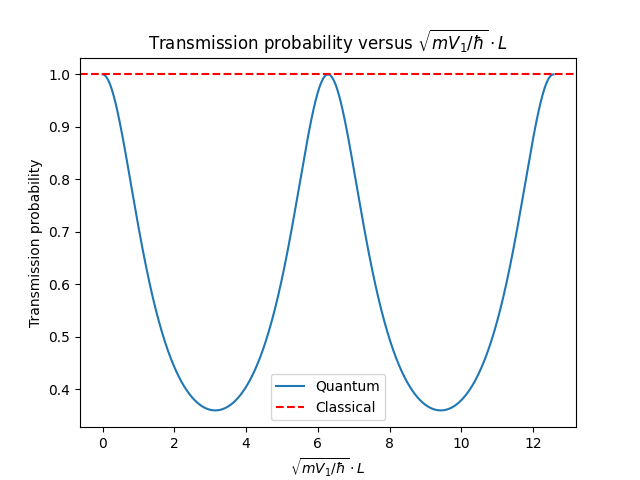
\includegraphics[width=0.8\textwidth]{A finite potential barrier T}
\end{figure}
\end{solbox}

\subsection*{7\lq Relativistic free fall (10 points)}
The action of a free falling relativistic particle under constant gravity $g$ is
\begin{align*}
S=\int \left(\a\sqrt{1-\frac{\dot{q}^{2}}{c^{2}}}-mgq\right)\,dt
\end{align*}
a) Determine the value of $\a$ by taking the Newtonian limit $\dot{q}\ll c$.\bigskip\newline
b) Show that the system has time translation symmetry.\bigskip\newline
Hint: note that
\begin{align*}
\frac{d}{dt}\left(-\sqrt{1-\frac{\dot{q}^{2}}{c^{2}}}\d t\right)=\frac{1}{c^{2}}\left(1-\frac{\dot{q}^{2}}{c^{2}}\right)^{-\frac{1}{2}}\dot{q}\ddot{q}\d t
\end{align*}
c) Derive the conserved quantity of time translation.\bigskip\newline
d) Determine if the system has space translation symmetry $q(t)\to q(t)+\e$.

\begin{solbox}
a) (2 points)\\
By Taylor expansion,
\begin{align*}
S=\a \int\sqrt{1-\frac{\dot{q}^{2}}{c^{2}}}\,dt\approx\int\left[\a\left(1-\frac{1}{2}\frac{\dot{q}^{2}}{c^{2}}\right)-mgq\right]\,dt
\end{align*}
Comparing with the Lagrangian in Newtonian mechanics, $\La=\frac{1}{2}m\dot{q}^{2}-mgq$, we know $\a=-mc^{2}$.\bigskip\newline
b) (3 points)\\
Time translation can be written as $q(t)\to q(t)+\e \dot{q}(t)\d t$, so $\d q=\dot{q}\d t\implies \d \dot{q}=\ddot{q}\d t$.
\begin{align*}
&\,\,\,\,\,\,\,-mc^{2}\sqrt{1-\frac{\left(\dot{q}+\e\d\dot{q}\right)^{2}}{c^{2}}}-mg\left(q+\e\d q\right)\\
&=-mc^{2}\sqrt{1-\frac{\dot{q}^{2}+2\e\dot{q}\d\dot{q}+\e^{2}\d\dot{q}^{2}}{c^{2}}}-mg\left(q+\e\d q\right)\\
&=-mc^{2}\sqrt{\left(1-\frac{\dot{q}^{2}}{c^{2}}\right)\left[1-\frac{2\e\dot{q}\d\dot{q}+\e^{2}\d\dot{q}^{2}}{\left(1-\frac{\dot{q}^{2}}{c^{2}}\right)c^{2}}\right]}-mg\left(q+\e\d q\right)\\
&\approx -mc^{2}\sqrt{1-\frac{\dot{q}^{2}}{c^{2}}}\left[1-\frac{1}{2}\cdot\frac{2\e\dot{q}\d\dot{q}+\e^{2}\d\dot{q}^{2}}{\left(1-\frac{\dot{q}^{2}}{c^{2}}\right)c^{2}}\right]-mg\left(q+\e\d q\right)\\
&=-mc^{2}\left(\sqrt{1-\frac{\dot{q}^{2}}{c^{2}}}-\frac{\e\dot{q}\d\dot{q}}{c^{2}\sqrt{1-\frac{\dot{q}^{2}}{c^{2}}}}\right)-mg\left(q+\e\d q\right)+\bigO\left(\d\dot{q}^{2}\right)
\end{align*}
The infinitesimal change in the Lagrangian is thus
\begin{align*}
\d\La&=-mc^{2}\left(\sqrt{1-\frac{\dot{q}^{2}}{c^{2}}}-\frac{\e\dot{q}\d\dot{q}}{c^{2}\sqrt{1-\frac{\dot{q}^{2}}{c^{2}}}}\right)-mg\left(q+\e\d q\right)+mc^{2}\sqrt{1-\frac{\dot{q}^{2}}{c^{2}}}+mgq\\
&=\frac{\e m\dot{q}\d\dot{q}}{\sqrt{1-\frac{\dot{q}^{2}}{c^{2}}}}-\e mg\d q\\
&=\frac{\e m\dot{q}\ddot{q}\d t}{\sqrt{1-\frac{\dot{q}^{2}}{c^{2}}}}-\e mg\dot{q}\d t\\
\implies \d S&=\e\int\left(\frac{m\dot{q}\ddot{q}\d t}{\sqrt{1-\frac{\dot{q}^{2}}{c^{2}}}}-mg\dot{q}\d t\right)\,dt
\end{align*}
Note that 
\begin{align*}
\frac{d}{dt}\left(-\sqrt{1-\frac{\dot{q}^{2}}{c^{2}}}\d t\right)=\frac{1}{c^{2}}\left(1-\frac{\dot{q}^{2}}{c^{2}}\right)^{-\frac{1}{2}}\dot{q}\ddot{q}\d t
\end{align*}
so
\begin{align*}
\d S&=\e\int\left[mc^{2}\frac{d}{dt}\left(-\sqrt{1-\frac{\dot{q}^{2}}{c^{2}}}\d t\right)-mg\frac{d}{dt}\left(q\d t\right)\right]\,dt\\
&=\e\int\frac{d}{dt}\left[\left(-mc^{2}\sqrt{1-\frac{\dot{q}^{2}}{c^{2}}}-mgq\right)\d t\right]\,dt\\
&=0
\end{align*}
We have dropped the total derivative term. The system has time translation symmetry.\bigskip\newline
c) (2 points)\\
From (b), we have $g=\left(mc^{2}\sqrt{1-\frac{\dot{q}^{2}}{c^{2}}}+mgq\right)\d t$. The conserved quantity is
\begin{align*}
Q&=g+\frac{\p \La}{\p \dot{q}}\d q\\
&=\left(mc^{2}\sqrt{1-\frac{\dot{q}^{2}}{c^{2}}}+mgq\right)\d t+\frac{m\dot{q}^{2}}{\sqrt{1-\frac{\dot{q}^{2}}{c^{2}}}}\d t\\
&=\left[\frac{mc^{2}\left(1-\frac{\dot{q}^{2}}{c^{2}}\right)+m\dot{q}^{2}}{\sqrt{1-\frac{\dot{q}^{2}}{c^{2}}}}+mgq\right]\d t\\
&=\left(\c mc^{2}+mgq\right)\d t
\end{align*}
The sum of relativistic energy and potential energy is thus conserved,
\begin{align*}
E=\c mc^{2}+mgq=\frac{Q}{\d t}
\end{align*}
d) (3 points)\\
Space translation is $q(t)\to q(t)+\e$. The infinitesimal change in the Lagrangian is
\begin{align*}
\d L&=-mc^{2}\sqrt{1-\frac{\dot{q}^{2}}{c^{2}}}-mg(q+\e)+mc^{2}\sqrt{1-\frac{\dot{q}^{2}}{c^{2}}}+mgq\\
&=-\e mg\\
\implies \d S&=\e\int-mg\,dt\\
&\neq 0
\end{align*}
This implies space translation is not a symmetry.
\end{solbox}

\subsection*{8\lq (Advanced) Information entropy (3 points)}
Compute the information entropy in the strings ``777", ``1416" and ``\textcolor{Lung Mun}{GLMMMNNUUUYY}". When computing probabilities for characters in a string, only consider the characters which appear in that string.

\begin{solbox}
For the first string ``777", $P(``7")=1$, so
\begin{align*}
H(``777")&=\log_{2}1\\
&=0
\end{align*}
For the second string ``1416", $P(``1")=\frac{1}{2}$ and $P(``4")=P(``6")=\frac{1}{4}$, so
\begin{align*}
H(``1416")&=\frac{1}{2}\log_{2}2+2\times\frac{1}{4}\log_{2}4\\
&=\frac{3}{2}
\end{align*}
For the third string ``\textcolor{Lung Mun}{\text{GLMMMNNUUUYY}}'', $P(``\textcolor{Lung Mun}{\text{G}}")=P(``\textcolor{Lung Mun}{\text{L}}")=\frac{1}{12}$, $P(``\textcolor{Lung Mun}{\text{M}}")=P(``\textcolor{Lung Mun}{\text{U}}")=\frac{1}{4}$ and $P(``\textcolor{Lung Mun}{\text{N}}")=P(``\textcolor{Lung Mun}{\text{Y}}")=\frac{1}{6}$, so
\begin{align*}
H(``\textcolor{Lung Mun}{\text{GLMMMNNUUUYY}}")&=2\times\frac{1}{12}\log_{2}12+2\times\frac{1}{4}\log_{2}4+2\times\frac{1}{6}\log_{2}6\\
&=\frac{7}{6}+\frac{1}{2}\log_{2}6
\end{align*}
\end{solbox}

\vfill
\centerline{\bf END OF PAPER}
\end{document}